\graphicspath{{/Users/Mike/phdthesis/MY_THESIS}}
\chapter{The CLAS detector at Thomas Jefferson National Accelerator Facility }\label{sec:clas}

The Thomas Jefferson National Accelerator Facility (\abbr{TJNAF}\label{abbr:tjnaf}, Fig.~\ref{fig:jlab.aerial}), also known as Jefferson Laboratory (\abbr{JLab}\label{abbr:jlab}) is located in Newport News, Virgina. It is one of 17 national laboratories funded by the U.S. Department of Energy and is home to three experimental halls, \desg{A}, \desg{B}, \desg{C}, and the Continuous Electron Beam Accelerator Facility,\cite{cebaf} (\abbr{CEBAF}\label{abbr:cebaf}, Fig.~\ref{fig:jlab.cebaf}).

\abbr{JLab}'s stated mission is ``to provide forefront scientific facilities, opportunities and leadership essential for discovering the fundamental structure of nuclear matter; to partner in industry to apply its advanced technology; and to serve the nation and its communities through education and public outreach."\cite{Jlabwiki} In addition to its science mission, the lab provides programs designed to help educate the next generation in science and technology, and to engage the public.
%\abbr{JLab} also conducts a variety of research using its Free-Electron Laser, which is based on the same electron-accelerating technology used in \abbr{CEBAF}.

The analysis performed in this work utilizes experimental data collected with the \abbr{CEBAF} Large Acceptance Spectrometer (\abbr{CLAS}) in hall \desg{B}, using \abbr{CEBAF}. The experiment \g12 collected over 126~TB of raw data in 44 days of beam time from April to June 2008, making \g12 the world's largest multi-particle dataset in the energy range 1.77 GeV $\mathrm{< \sqrt{s} <}$ 3.33 GeV. This chaper is dedicated to the explanation of \abbr{CEBAF}, \abbr{CLAS} and other subsystems used during the \g12 run period.


\begin{figure}[H]
%\begin{center}
\centering
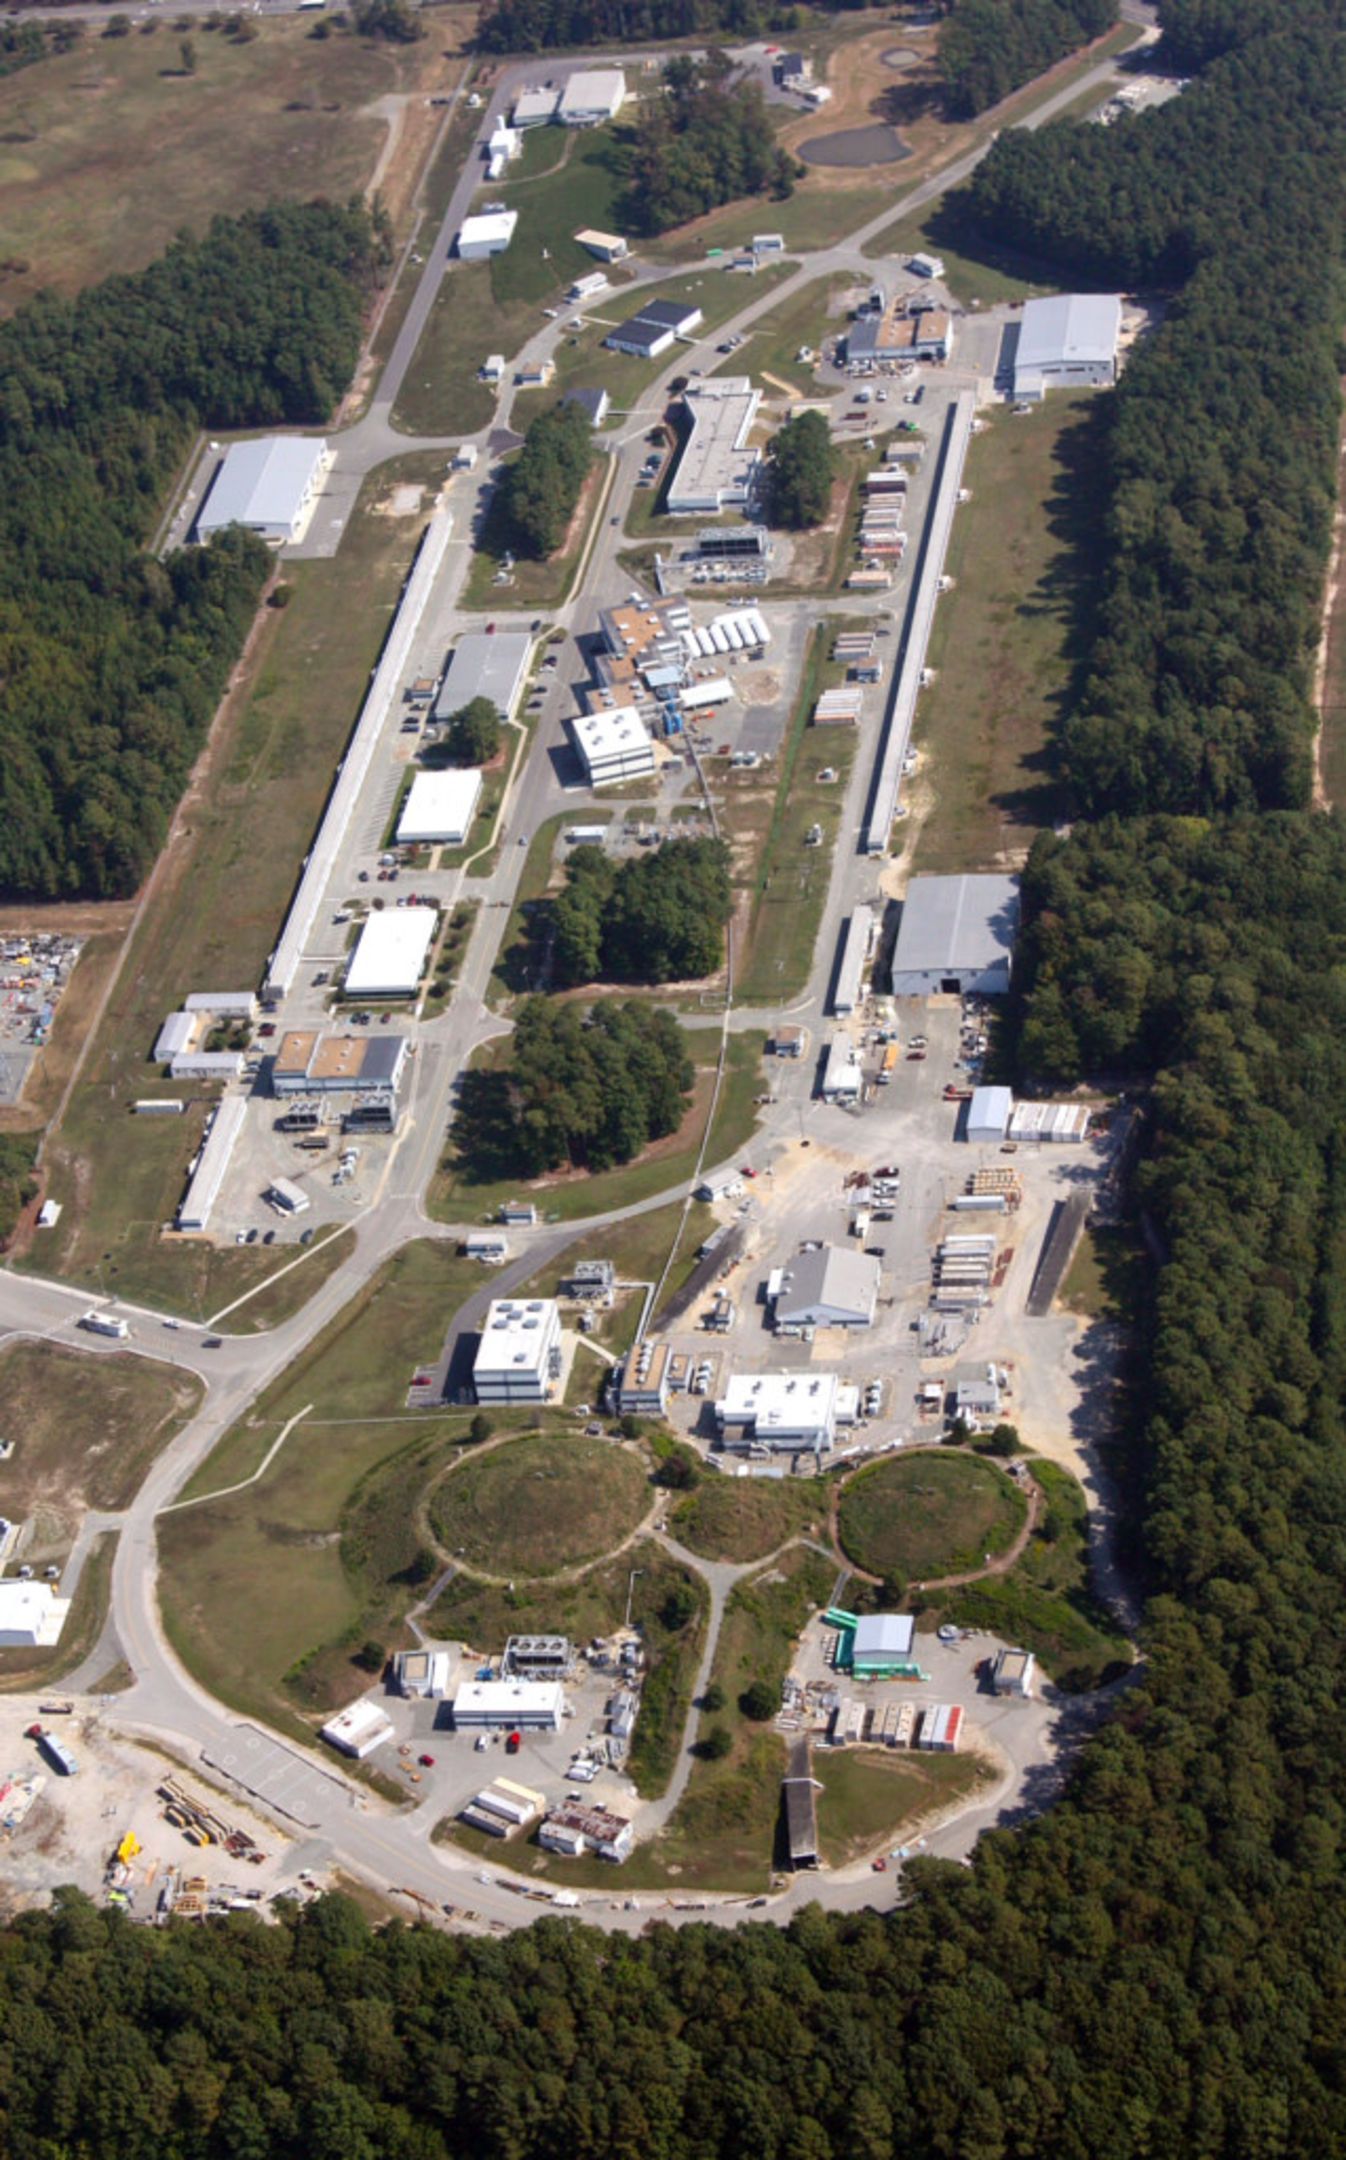
\includegraphics[width=0.6\columnwidth ,height=\hfigheight]{\grpath/jlab/jlab_arial_view_II.pdf}
\caption[Aerial view of Jefferson Laboratory (\abbr{JLab}) facing east]{\label{fig:jlab.aerial}Aerial view of Jefferson Laboratory (\abbr{JLab}) facing east. Image Source: \cite{cebafflckr}}
%\end{center}
\end{figure}
%
\begin{figure}\begin{center}
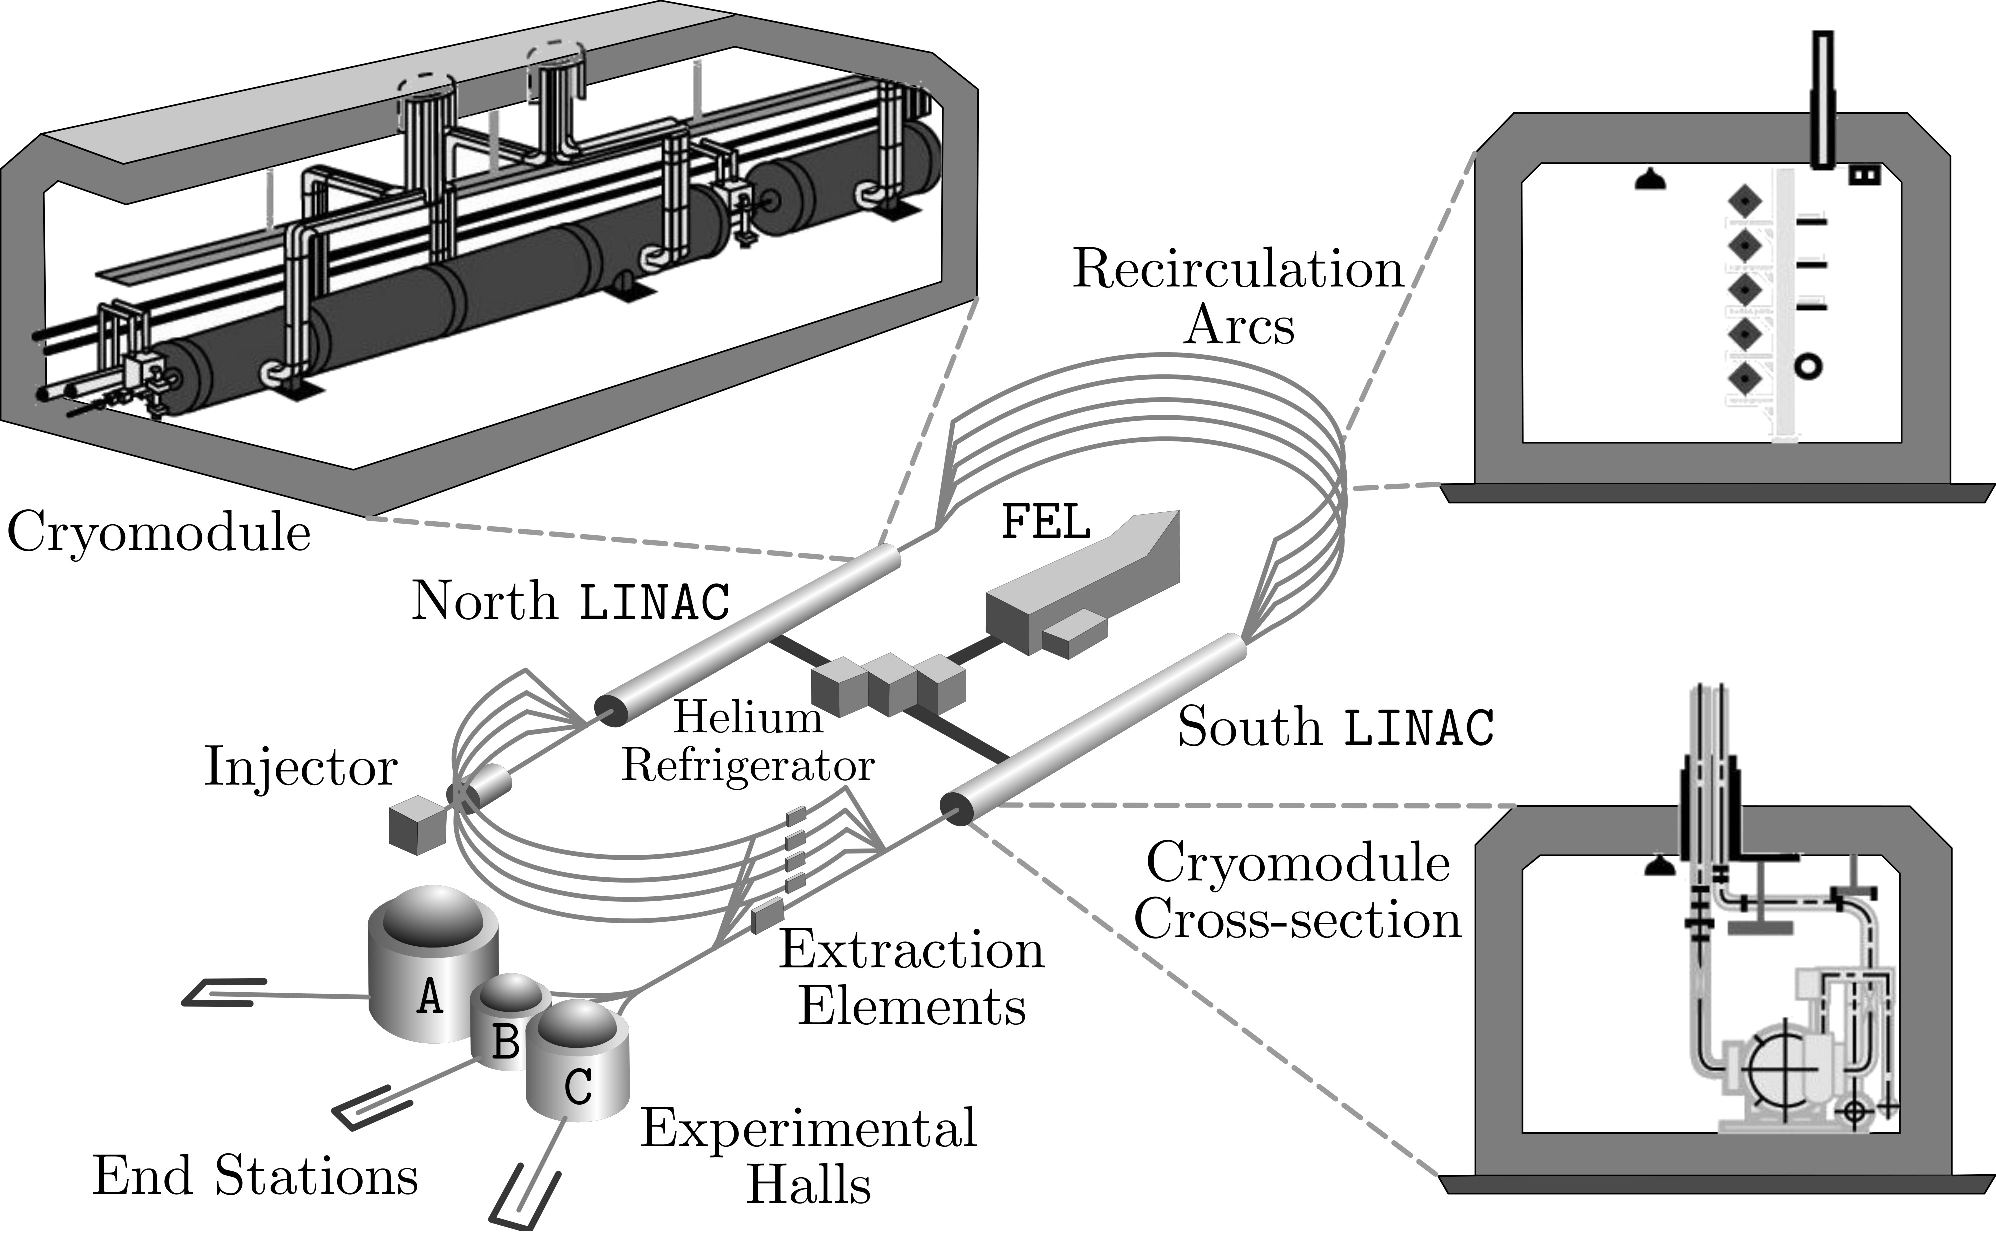
\includegraphics[width=0.9\columnwidth, height=\qfigheight]{\grpath/jlab/cebaf.pdf}
\caption[The Continuous Electron Beam Accelerator Facility (\abbr{CEBAF}) at Jefferson Laboratory (\abbr{JLab})]{\label{fig:jlab.cebaf}The Continuous Electron Beam Accelerator Facility (\abbr{CEBAF}) at Jefferson Laboratory (\abbr{JLab}) showing cross-sections of the linear accelerator (\abbr{LINAC}) halls and the recirculation arcs. Also depicted are the Free Electron Laser (\abbr{FEL}\label{abbr:fel}) and the helium refrigerator and distribution facility. Image Source:\cite{cebaf}}
\end{center}\end{figure}
\FloatBarrier
\section{Continuous Electron Beam Accelerator Facility}\label{sec:cebaf.desc}

\abbr{CEBAF} utilizes superconducting radio-frequency (\abbr{srf}\label{abbr:srf}) cavities to accelerate electrons and provide a continuous wave beam with 75\% polarization to the three halls simultaneously. A list of some specifications for \abbr{CEBAF} can be found in Table~\ref{tab:cebafspecs}.
%Niobium (\abbrlc{N}{b}\label{abbr:nb}), in a cryogenic system, provides the superconducting environment necessary for \abbr{CEBAF} to obtain a 100\% duty factor because superconducting cavities are non-resistive. Prior to the implementation of \abbr{srf}, copper \abbr{RF}\label{abbr:rf} cavities were used, however due to the resistive properties of copper significant cooling time was needed due to heat produced in the cavity.
\begin{table}
\begin{minipage}{\textwidth}
\begin{center}
\begin{singlespacing}

\caption[\abbr{CEBAF} Operating Specifications]{\label{tab:cebafspecs}Operating specifications of \abbr{CEBAF} at \abbr{JLab}.\cite{cebaf}}

\begin{tabular}{c|c}

%\hline \hline
%
%operation & \multicolumn{3}{c}{Generation} \\
%charge & I & II & III \\


\hline

$\textrm{E}_{min}$ & 0.6 GeV \\
$\textrm{E}_{max}$ & 6.0 GeV \\
$\textrm{I}_{max}$ & 200 $\mu$A \\
Polarization & $\textgreater$ 75\% \\
Geometric emittance & $\textless \ 10^{9}$ m rad \\
Momentum Spread & $10^{-5}$ \\
Average currents (Halls A and C) & 1-150$\mu$A \\
Average currents (Hall B) & 1-100nA \\
Bunch charge & $\textless$ pC \\
Repetition rat & 499 MHz/hall \\ 
Beam size (rms transverse) & $\sim$ 80 $\mu$m \\
Bunch length (rms) & 300 fs, 90 $\mu$m \\
Energy spread & 2.5 x 10$^5$ \\
Beam power & $\textless$ \ MW  \\
Beam loss & $\textless \mu$A  \\
Number of passes & 5 \\
Number of accelerating cavities & 338 \\
Fundamental mode frequency & 1947 MHz \\
Accelerating cavity effective length & 0.5m \\
Cells/cavity  & 5\\
Average $Q_{0}$  & 4.0 x 10$^9$ \\
Implemented $Q_{ext}$  & 5.6 x 10$^6$ \\
Cavity impedance (r/Q)  & 980 $\Omega$ \\
Average cavity accelerating gradient  & 7.5 MV/m \\
RF power  & $\textless$ \ 3.5 kW/cavity \\
Amplitude control  & 1.00 x 10$^{-4}$ rms \\
Phase control  & 0.1$^\circ$ rms \\
Cavity operating temperature  &  2.08 K\\
Heat load @ 2 K  &  $\textless$ 9 W/cavity\\
Liquefier 2 k cooling power  & 5kW \\
Liquefier operating power  &  5MW\\




\hline \hline

\end{tabular}

\end{singlespacing}
\end{center}
\end{minipage}
\end{table}
\vspace{20pt} 

To achieve the running conditions described in Table~\ref{tab:cebafspecs} \abbr{CEBAF} uses a GaAs photocathode laser driven injector system to produce a highly polarized electron beam. The laser pulses create three electron bunches that are bunched together in 2 ns groups, about 90 $\mu$m in length. Each bunch is 499~MHz at the source at 100 keV, spaced apart by 120$^\circ$ of \abbr{rf} phase. Together the electron bunches form a 1497 MHz beam that then enters two 1/4 \abbr{srf} cavities which accelerate the electrons to $\sim$1\% of the total machine energy before it is injected into the \abbr{CEBAF}'s main accelerator. 

When the electron bunches enter the \abbrlc{N}{b} \abbr{srf} cavity, they undergo an acceleration gradient provided by \abbr{rf} standing wave established inside of the cavity. The standing waves are kept in phase with the electron bunches resulting in a continuous positive electric force on each bunch as it passed through a cavity, see Fig.~\ref{fig:jlab.accel}

\begin{figure}\begin{center}
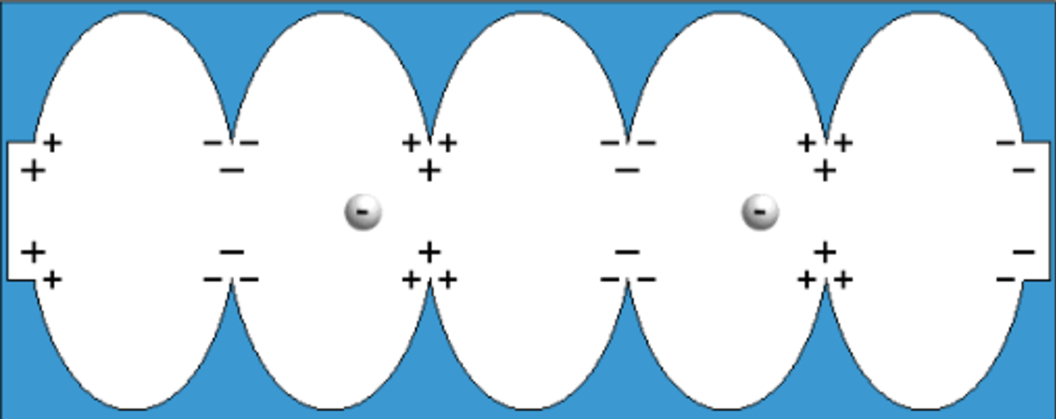
\includegraphics[width=0.8\figwidth,height=\qfigheight]{\grpath/jlab/accelerating_diagram.pdf}
\caption[Accelerating Cavity Diagram]{\label{fig:jlab.accel}Accelerating Cavity Diagram. Electron clusters experience a continuous acceleration due to a standing electromagnetic wave indicated by the positive and negative signs along the inner wall.}
\end{center}\end{figure}

The main accelerator, Fig.~\ref{fig:jlab.cebaf}, consists of a pair of linear accelerators (\abbr{LINAC}s\label{abbr:linac}). Each \abbr{LINAC} contains 168 \abbr{srf} \abbrlc{N}{b} cavities that are submerged in liquid Helium and cooled to 2.08 K, the temperature by which \abbrlc{N}{b} becomes superconducting. In total there are twenty cryogenic modules, each containing eight superconducting niobium cavities as depicted. in Fig.~\ref{fig:jlab.cavity}. 
%The significant cooling requirements are satisfied by the Lab's Central Helium Liquefier (\abbr{CHL}\label{abbr:chl}). 


\begin{figure}\begin{center} 
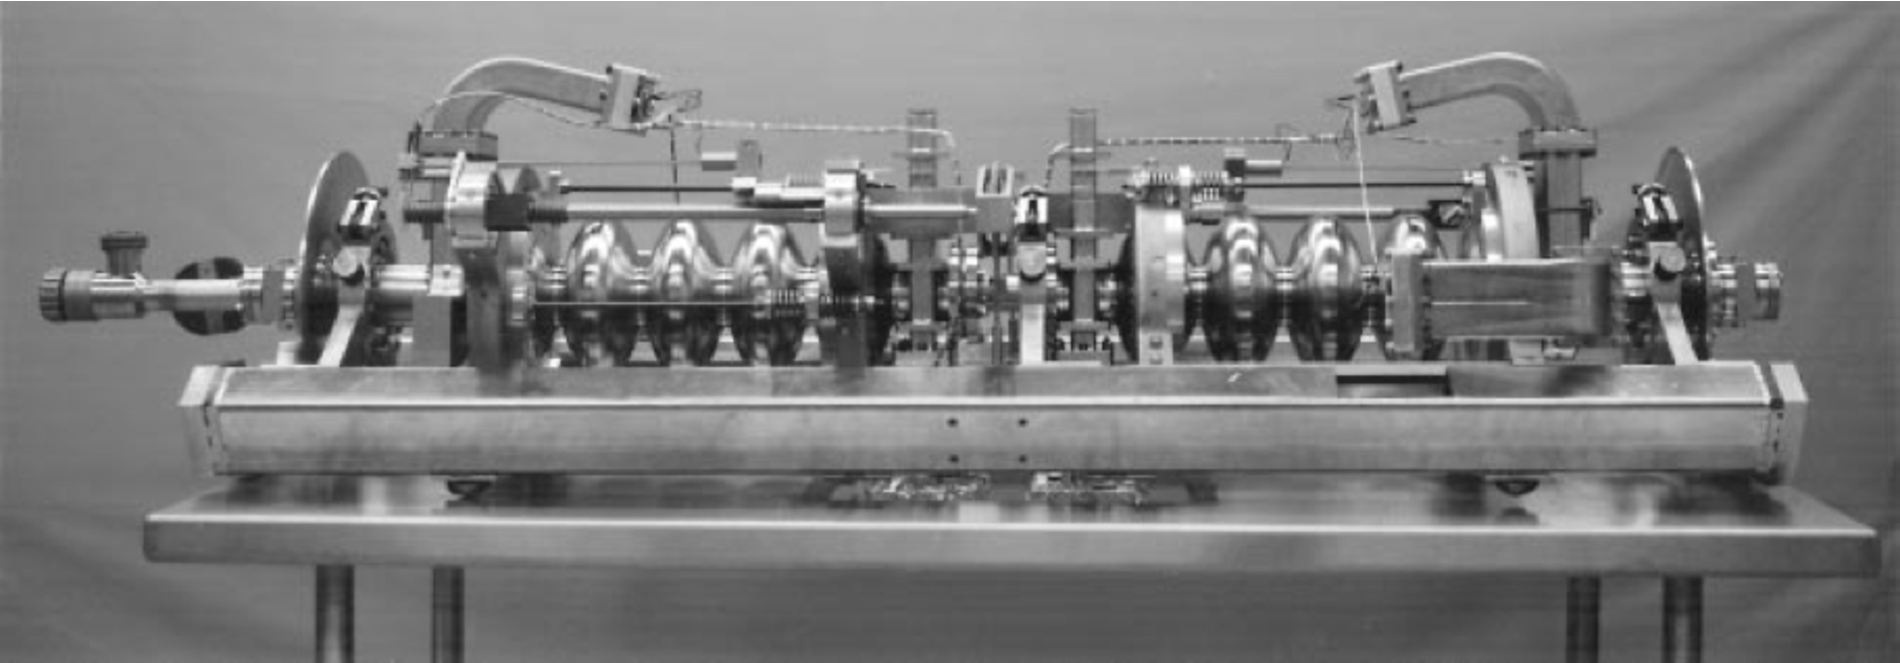
\includegraphics[width=\figwidth, height=\qfigheight]{\grpath/jlab/niobium_cavity_pair.pdf}
\caption[A \abbr{CEBAF} superconducting niobium cavity pair]{\label{fig:jlab.cavity}A \abbr{CEBAF} superconducting niobium cavity pair. Image Source: \cite{cebaf}}
\end{center}\end{figure}

The beam, once inside the \abbr{LINAC} can be passed up to five times. The \abbr{LINAC}s are connected by two sets of 180$^\circ$ magnetic-dipole bending arcs (see Fig.~\ref{fig:jlab.cebaf}) with a radius of 80~meters. The beam is sent through both accelerators and is then recirculated up to four more times. Each \abbr{LINAC} is capable of accelerating the beam by up to 600~MeV giving approximately 1.2~GeV per pass. Each hall can choose to extract the beam after any number of passes, however the fifth (final) pass can be sent to all three halls simultaneously. It should be noted that although each hall can receive the fifth pass, no two halls can run with the same lower energy \cite{clas.pass}. At the time of the \g12 experiment, the accelerator was capable of delivering a maximum electron beam energy of 5.714~GeV.
%\FloatBarrier
%\FloatBarrier
\section{Circular Polization} \label{sec:clas.polar}

As mentioned in Sec.~\ref{sec:cebaf.desc}, the electron beam provided by \abbr{CEBAF} has the capability of having 75\% longitudinal polarization. Longitudinal polarized electrons produce circularly polarized photons in the bremsstrahlung process on any target, however intensity of photon beam depends on Z of target. The circular polarization production process is quantum mechanical. From QED calculations, the degree of circular polarization transfer to the photon, $P_{circ}$, is seen to depend on the ratio of the relative electron energy to the bremsstrahlung photon, $\epsilon$:
%The experiment \g12 used a Au foil as a radiator therefore \g12 had a circular polarized beam.
\begin{equation}\label{eq:polarization}
	P_{circ} = (\frac{4\epsilon - \epsilon^{2}}{4-4\epsilon+3\epsilon^{2}})P_{e} \cite{Olsen}
\end{equation}
where $\epsilon = k/E_{0}$, $k$ is the bremsstrahlung photon energy and $E_{0}$ is the incident electron energy. Equation~\ref{eq:polarization} shows that circular polarization of the photon is transferred directly from the polarization of the electron, it also shows that the atomic nucleus or radiator plays no role in transfer of polarization. The transfer of circular polarization is maximum at the higher end of the energy spectrum $\epsilon$ and decreases towards the lower end of the spectrum as seen in Fig.~\ref{fig:jlab.polarization}. Figure~\ref{fig:jlab.polarization} also illustrates that polarization transfer is favored when the radiated photons take up large fractions of the incident electron energy. Coulomb and screening corrections (due to the atomic electrons) do not significantly affect the polarization of the emitted photons. 

\begin{figure}[h!]\begin{center}
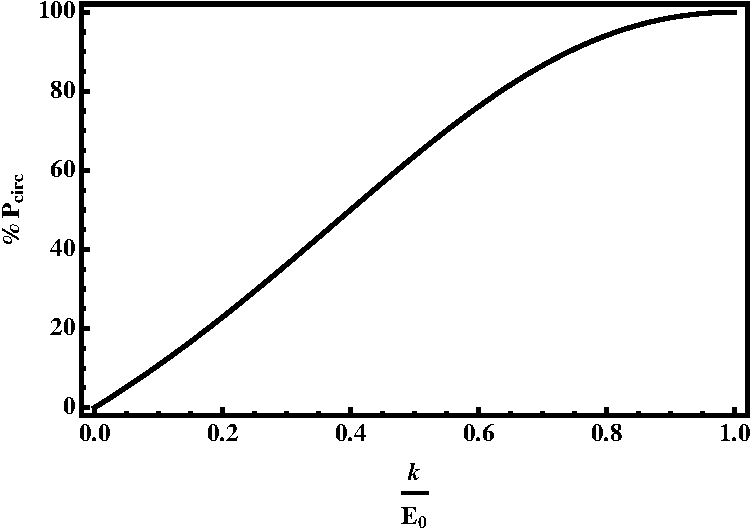
\includegraphics[width=0.8\figwidth,height=\qfigheight]{\grpath/hall-b/polarization.pdf}
\caption[Circular polarization Graph]{\label{fig:jlab.polarization}QED calculation for the degree of circular polarization of 50-MeV electrons in lead. The curve shown is a Born-approximated calculation which neglects screening corrections. An exact calculation involving Coulomb and screening corrections (not shown) yields similar results.\cite{Olsen}}
\end{center}\end{figure}

\FloatBarrier
\section{Beam Positioning}\label{sec:clas.beam}
%\FloatBarrier
There are several beam monitoring stations in Hall \desg{B} before and after the \abbr{CLAS} detector (Fig.~\ref{fig:clas.beam.beforemonitors}) to scan the important details of the electron beam prior to conversion into a photon beam and the details of the photon beam before and after entering the target. Such quantities for the electron beam include position, intensity, dispersion, and current, and for the photon beam include position, dispersion and flux. Most of these monitoring stations are used by the accelerator group.
% to steer the beam to the target as they control all magnets that can substantially move the beam.
\begin{figure}[h!]\begin{center}
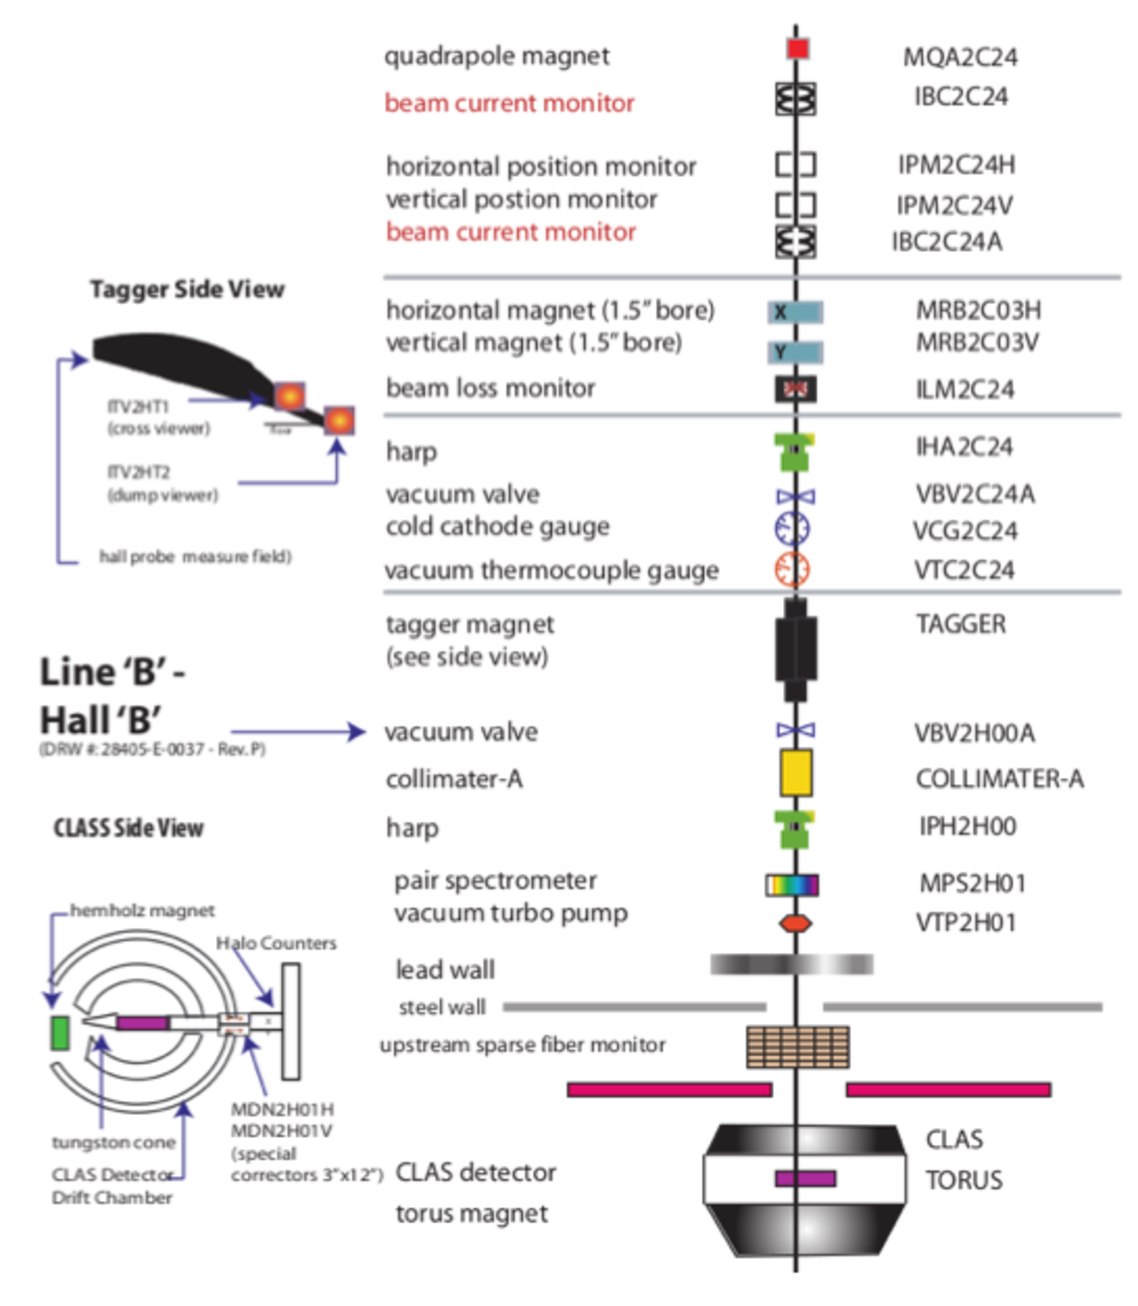
\includegraphics[width=\figwidth, height=1.75\hfigheight]{\grpath/hall-b/beamline_components.pdf}
\caption[Beamline and components of \abbr{CLAS}]{\label{fig:clas.beam.beforemonitors}{\coloronline}Beamline and components of \abbr{CLAS}. Image Source~\cite{cebafflckr}}
\end{center}\end{figure}
There are two types of devices to measure the electron beam position. The first type is represented by two beam position monitors (\abbr{BPM}s\label{abbr:bpm}) placed before the tagger. The position monitors use three radiofrequency cavities to measure the transverse location of the electron beam and its intensity. This information is used as feedback for the steering mechanism. The position monitors are noninvasive and measure at a rate of 1 Hz. 
The second type of device used to measure the beam position is the Harp Beam Profile Monitor, which also measures the electron beam dispersion. The harp devices consist of fine wires (20 and 50~{\um} W and 100~{\um} Fe) that can be passed through the beam at specific orientations and collect scattered electrons with a photomultiplier tube. This procedure measures the horizontal ($x$) and vertical ($y$) profile of the electron beam and is performed after any downtime or change in the beam. The accelerator group adjusts the beam position such that more than 99\% of the electron beam goes through the radiator. Since this process is invasive, it was only done when the drift-chambers and \abbr{DAQ} were turned off. A harp scan measurement for \g12 is shown in Fig.~\ref{fig:clas.beam.harpscan}. The width of the beam was contained within a 200 $\mathrm{\mu}$m diameter.



%\begin{figure}\begin{center}
%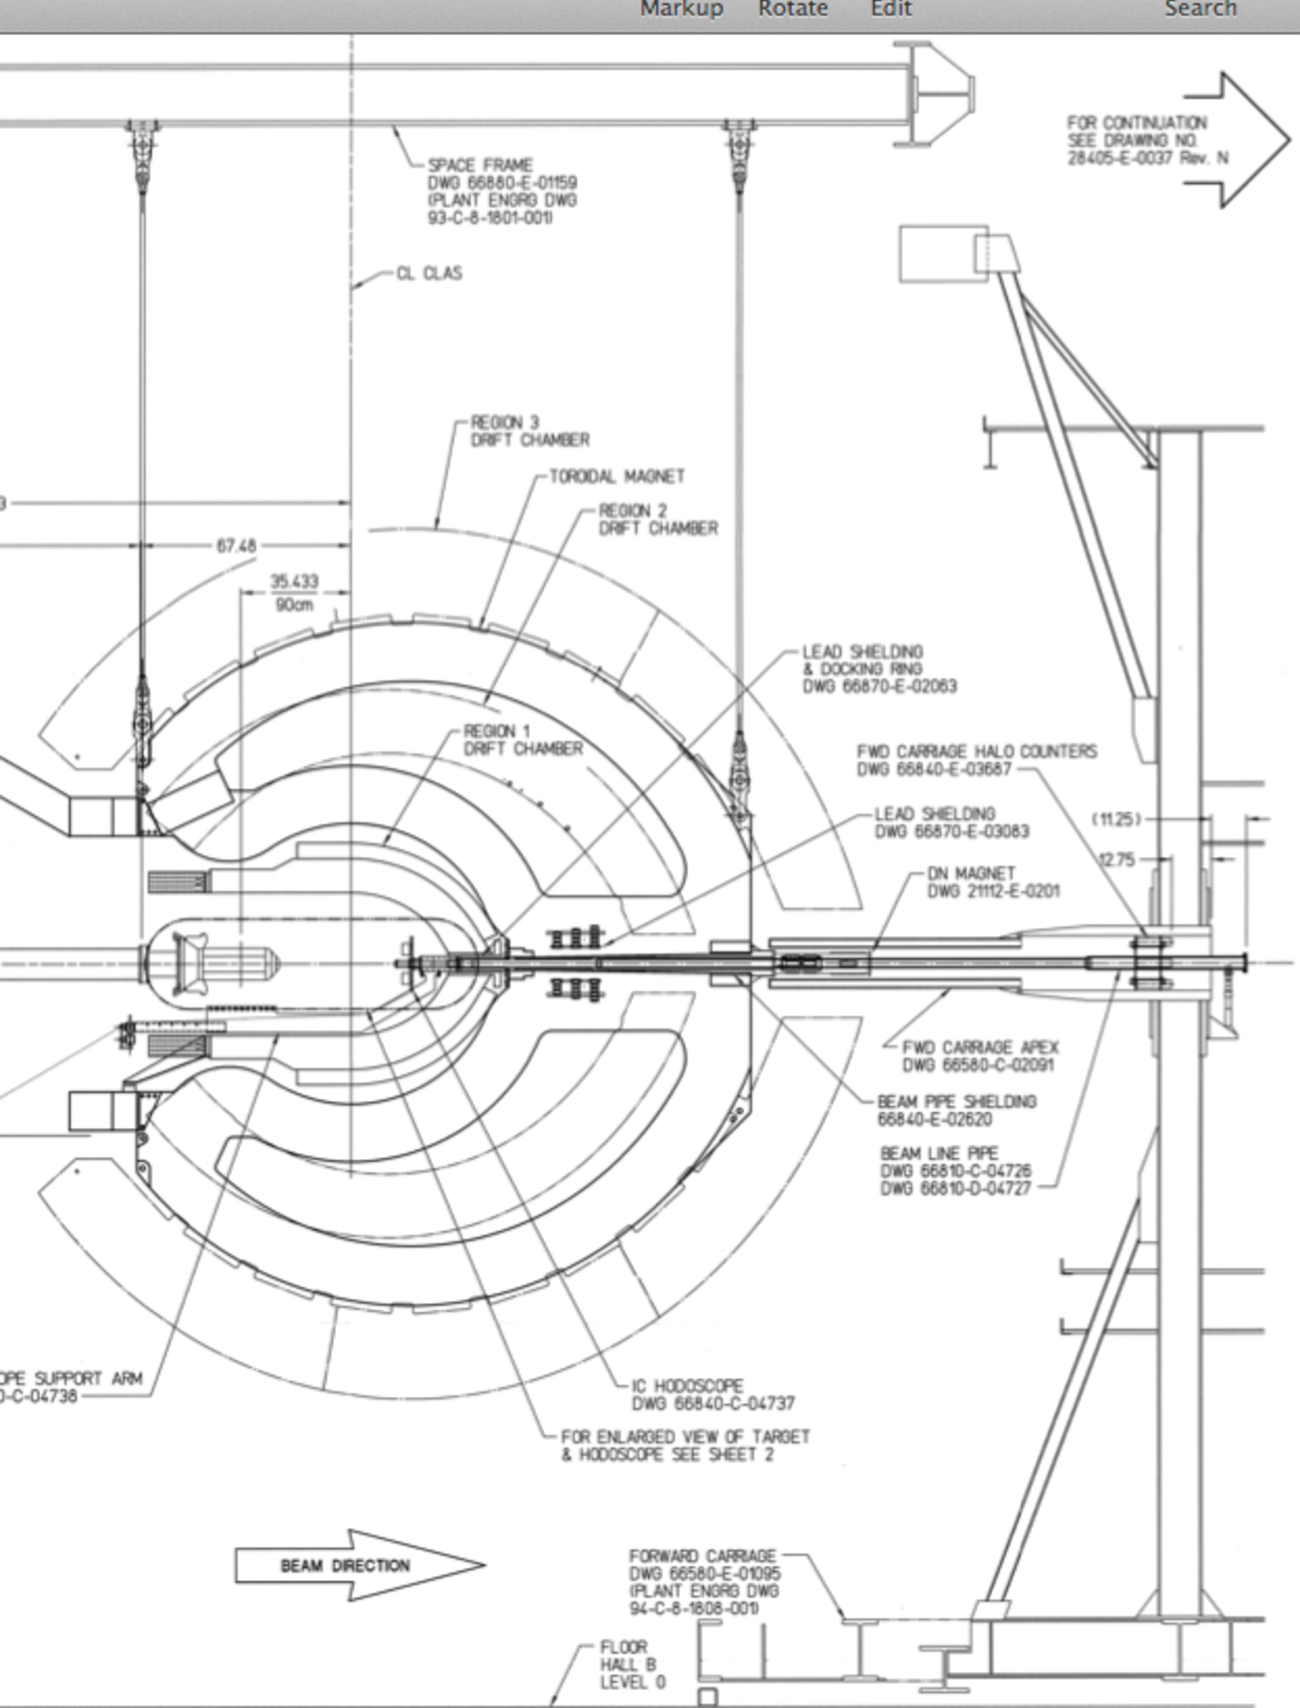
\includegraphics[width=\figwidth,height=\hfigheight]{\grpath/hall-b/G12_afterbeam_blueprint.pdf}
%\caption[Beamline and \abbr{CLAS} components in \g12]{\label{fig:clas.beam.aftermonitors}{\coloronline}Beamline and \abbr{CLAS} components in \g12}
%\end{center}\end{figure}

\begin{figure}\begin{center}
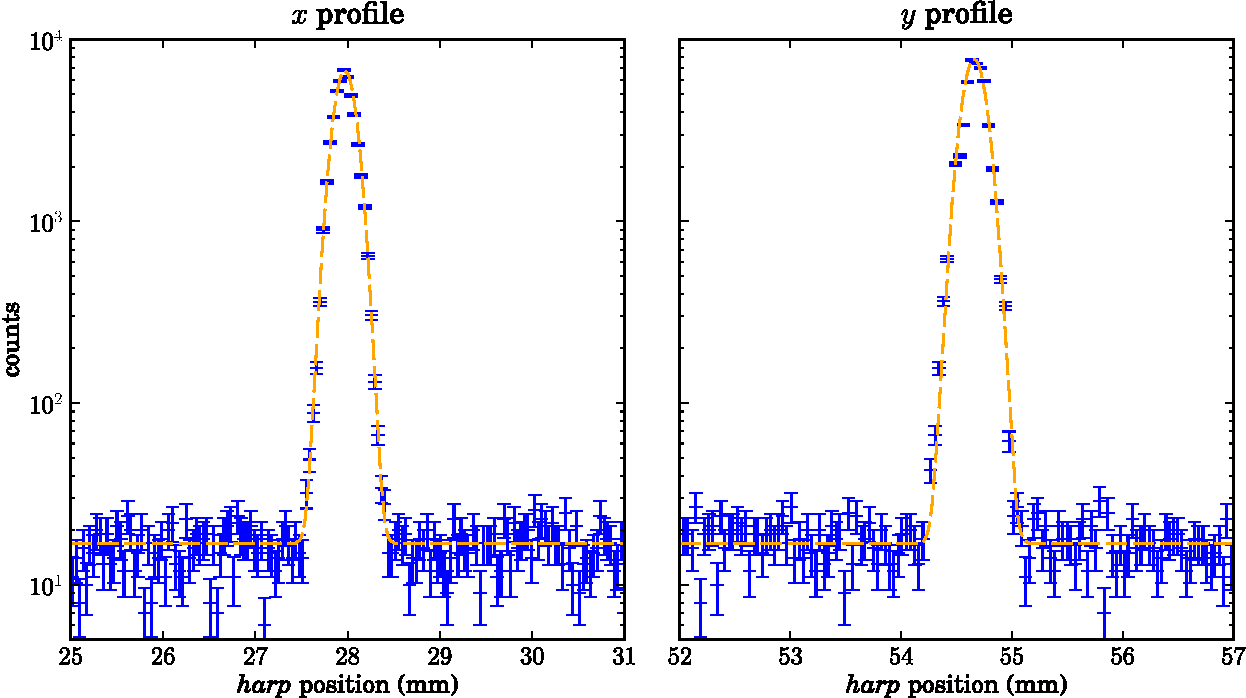
\includegraphics[width=\figwidth,height=\qfigheight]{\grpath/calibration/harpscan.pdf}
\caption[A typical \emph{harp} scan done just prior to run 56426]{\label{fig:clas.beam.harpscan}{\coloronline}A typical \emph{harp} scan done just prior to run 56426. Shown are the $x$ and $y$ profiles of the electron beam just before the tagger. The dashed orange line is a Gaussian fit to the data: $\sigma_x~=~0.115$~mm and $\sigma_y~=~0.105$~mm. Image Source:~\cite{goetz}}
\end{center}\end{figure}

The Total Absorption Shower Counter located downstream of \abbr{CLAS}, measures the photon flux (see Fig.~\ref{fig:clas.beam.afterCLAS}). The \abbr{TASC}, consists of four lead glass blocks of $\sim$ 17 radiation lengths, each coupled to a photo-multiplier tube (\abbr{PMT}\label{abbr:pmt}). The \abbr{TASC} is approximately 100\% efficient at detecting photons at beam currents less than 100~pA\cite{clas.tagger,clas.tagger.calib}. Since \g12 ran with 65~nA current, special low current, 50~pA, normalization runs(see Table~\ref{tab:data.calibruns}) were taken several times throughout \g12. The ratio of electrons detected in the photon tagger (see Sec.~\ref{sec:clas.tagr}) to that of photons detected in the \abbr{TASC} gives the tagging ratio used to calibrate the tagger and measure the flux throughout the entire \g12 run period.
%with hits in the left and right \abbr{TDC} matching in time and a corresponding hit in an E-counter
\begin{figure}[h!]\begin{center}
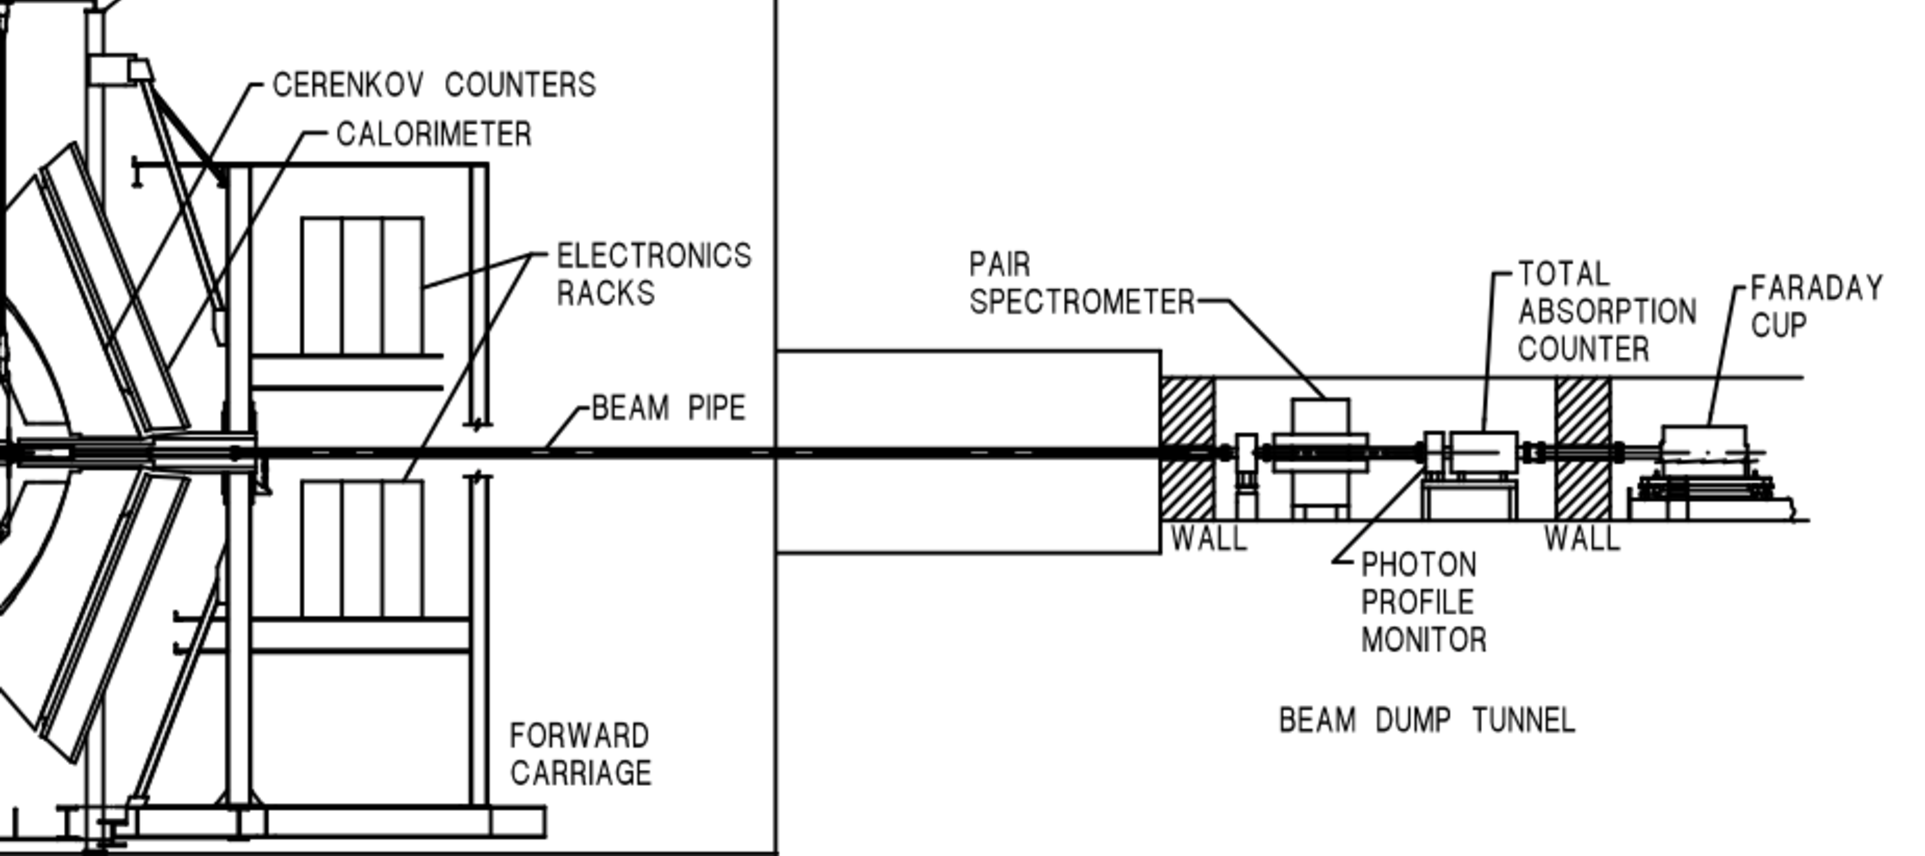
\includegraphics[width=\figwidth,height=0.8\qfigheight]{\grpath/hall-b/TASC_blueprint.pdf}
\caption[Beamline and components after \abbr{CLAS} ]{\label{fig:clas.beam.afterCLAS}{\coloronline}Beamline components in \g12 after \abbr{CLAS}}
\end{center}\end{figure}

\FloatBarrier
\section{Photon Tagger} \label{sec:clas.tagr}

The electron beam delivered to hall \desg{B} from \abbr{CEBAF} can be sent directly to a target or the electron beam can produce a \emph{real photon} beam by means of bremsstrahlung radiation by passing the electron beam through a radiator. Typical radiators have high atomic number to help reduce contamination of photons produced by electron-electron scattering. The \g12 experiment used a gold (\abbrlc{A}{u}) foil of $10^{-4}$~radiation length. This choice has a double purpose, to maximize the probability of the electron-nucleus interaction given that the bremsstrahlung cross section is proportional to $\mathrm{Z^{2}}$, and to minimize the number of interaction centers such that each electron interacts once, producing only one photon. After the electron beam passes through the radiator, the beam becomes a mixture of photons and electrons that did not interact with the radiator and recoil electrons. The mixed beam then travels into a dipole magnetic field which sweeps the electrons out of the electron-photon beam. The electrons present in the electron-photon beam are directed toward two hodoscope planes, each made of an overlapping array of scintillators to detect the energy-degraded electrons.

%  

The first scintillator plane, referred to as the E-plane (Figs.~\ref{fig:jlab.tagr.energies}, and~\ref{fig:jlab.tagr.paddles}), is used to determine the momentum of the recoiling electrons. The E-plane provides photon energy resolution on the order of 0.1\% of the incident electron beam energy. It consists of 384 paddles that are 20 cm long, 4 mm thick and from 6 to 18 mm wide. The paddles are arranged in an overlapping fashion, thus increasing the number of logical paddles to 767.
The trajectory of an electron or any charged particle in the magnetic field is governed by the equation
\begin{equation}\label{eq:motioninmag}
	p = qrB \ (\mathrm{if}\ \vec{p} \perp \vec{B} )
\end{equation}
where $p$ is the particle's momentum, $q$ is the particle's charge, $r$ is the particle's radius of curvature and $B$ is the magnetic field the particle passes through.
By determining which paddle an electron hit we know the radius of curvature and we can calculate the momentum of the electron. The momentum of the electron can then be used to obtain the energy of the photon by means of the conservation relation 
\begin{equation}\label{eq:tagger.energy}
	E_{\gamma} = E_{0} - E_{e}
\end{equation}
where $E_{0}$ is the energy of the incident electron given by \abbr{CEBAF}, $E_{e}$ is the energy of the recoil electron and $E_{\gamma}$ is the energy of the emitted photon. 

The second scintillator plane, referred to as the T-plane, is used to make accurate timing measurements of the recoiling electrons. This plane comprises of 61 paddles that are each 2 cm thick. The added thickness of these paddles allow for a timing resolution of 110 ps.
% The spectrometer was able to tag photons ranging from 20-95\% of the incident electron beam energy.

The tagger can tag photons of energies from 20 to 95\% of the incident electron beam energy. For \g12 this corresponds to a photon energy range of 1.142 - 5.425~GeV. Due to the high current of the electron beam delivered to \g12 from \abbr{CEBAF} there were usually more than one ``hit'' in the tagger for each event. Normally, the one associated with the photon that caused the event could be obtained by a timing coincidence with the tracks, although there are cases when this photon is ambiguous as discussed in Sec.~\ref{sec:analysis.beam}.

The photons that pass through the radiator then pass through a 6.2~mm diameter collimator. Collimation is used to trim the beam halo prior to arriving at the CLAS cryotarget. In the \g12 experiment the beam entering the cryotraget was 1.5~cm in radius. The collimator was positioned 537~cm upstream of the cryotarget which had a radius of 2~cm. A sweeping magnet were placed after the collimator to remove any charged particles created by interactions of photons with the collimator.

More detailed information on the Hall B tagging system and \abbr{DAQ} of the tagger system can be found in \cite{clas.tagger}.

\begin{figure}\begin{center}
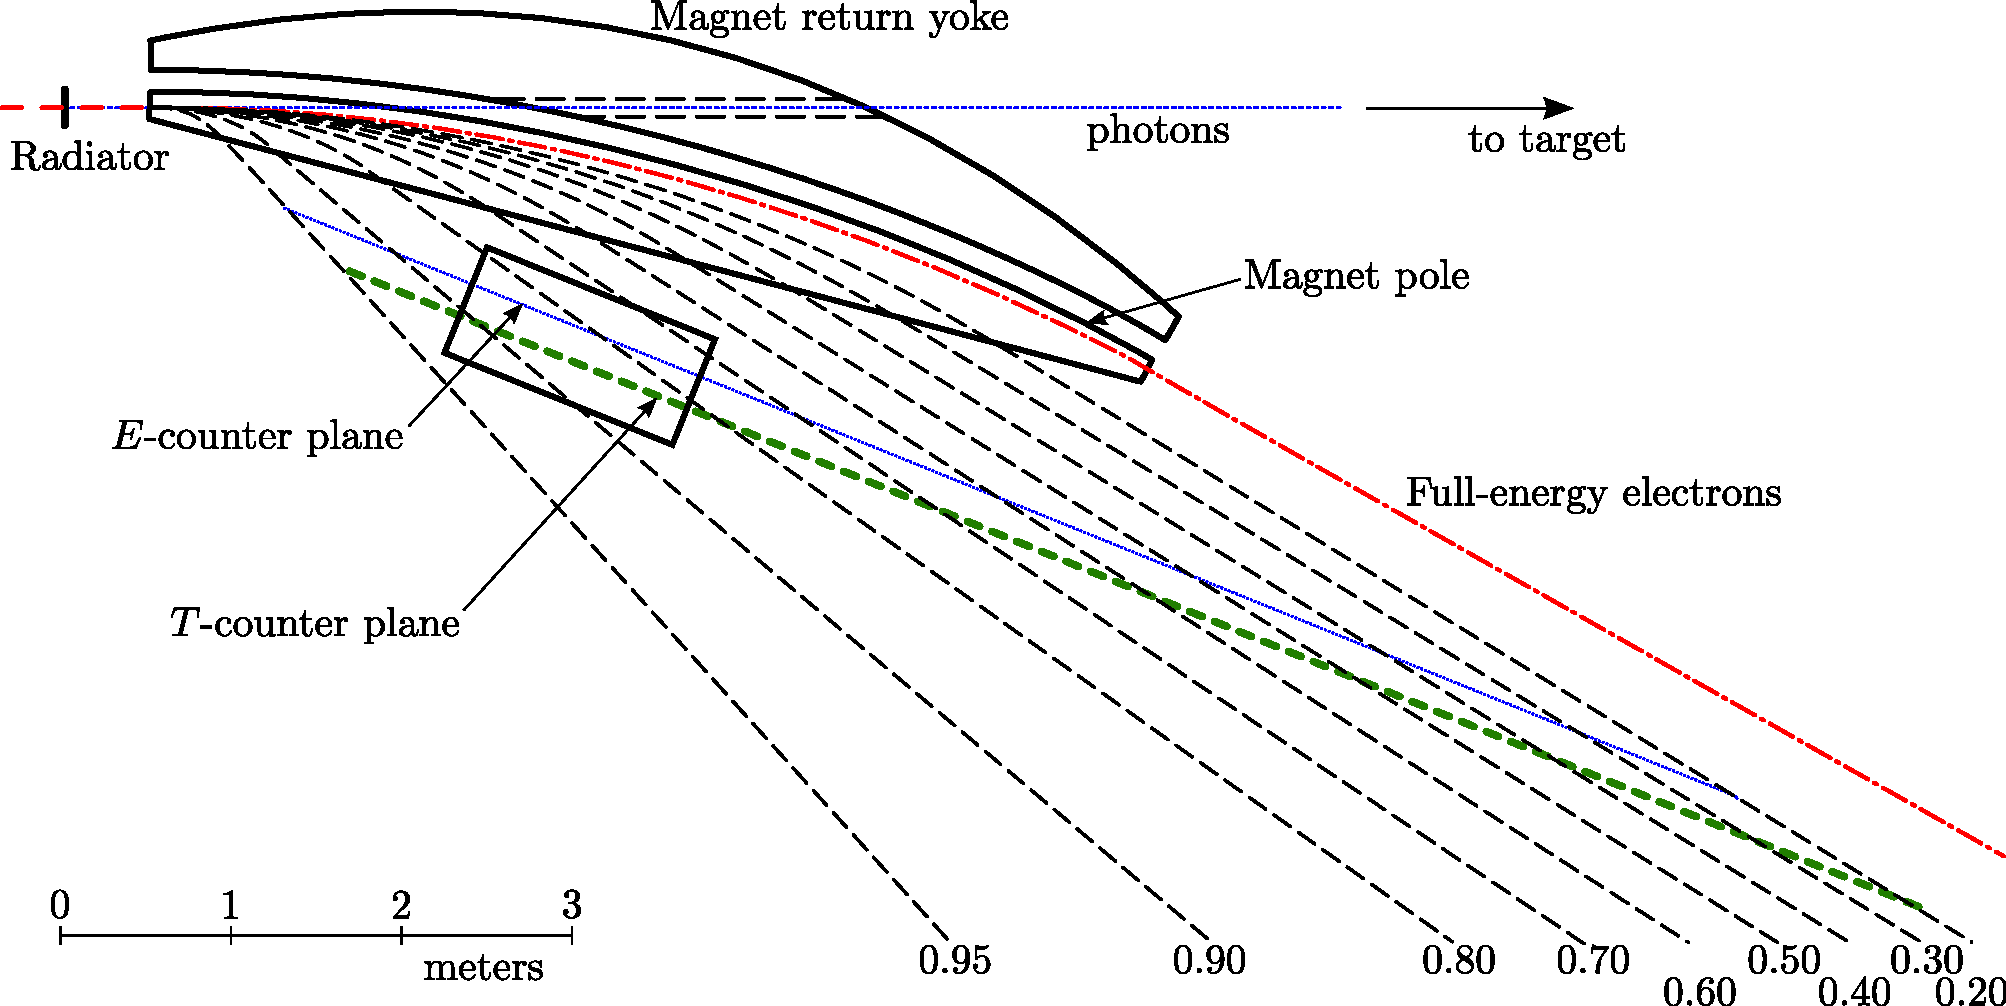
\includegraphics[width=0.8\figwidth,height=\qfigheight]{\grpath/hall-b/tagger_energies.pdf}
\caption[Scale drawing of the photon tagger system]{\label{fig:jlab.tagr.energies}Scale drawing of the photon tagger system. The rectangular area around the $E$ and $T$-counter planes outlines the expanded view shown in Fig.~\ref{fig:jlab.tagr.paddles}.}
\end{center}\end{figure}


\begin{figure}\begin{center}
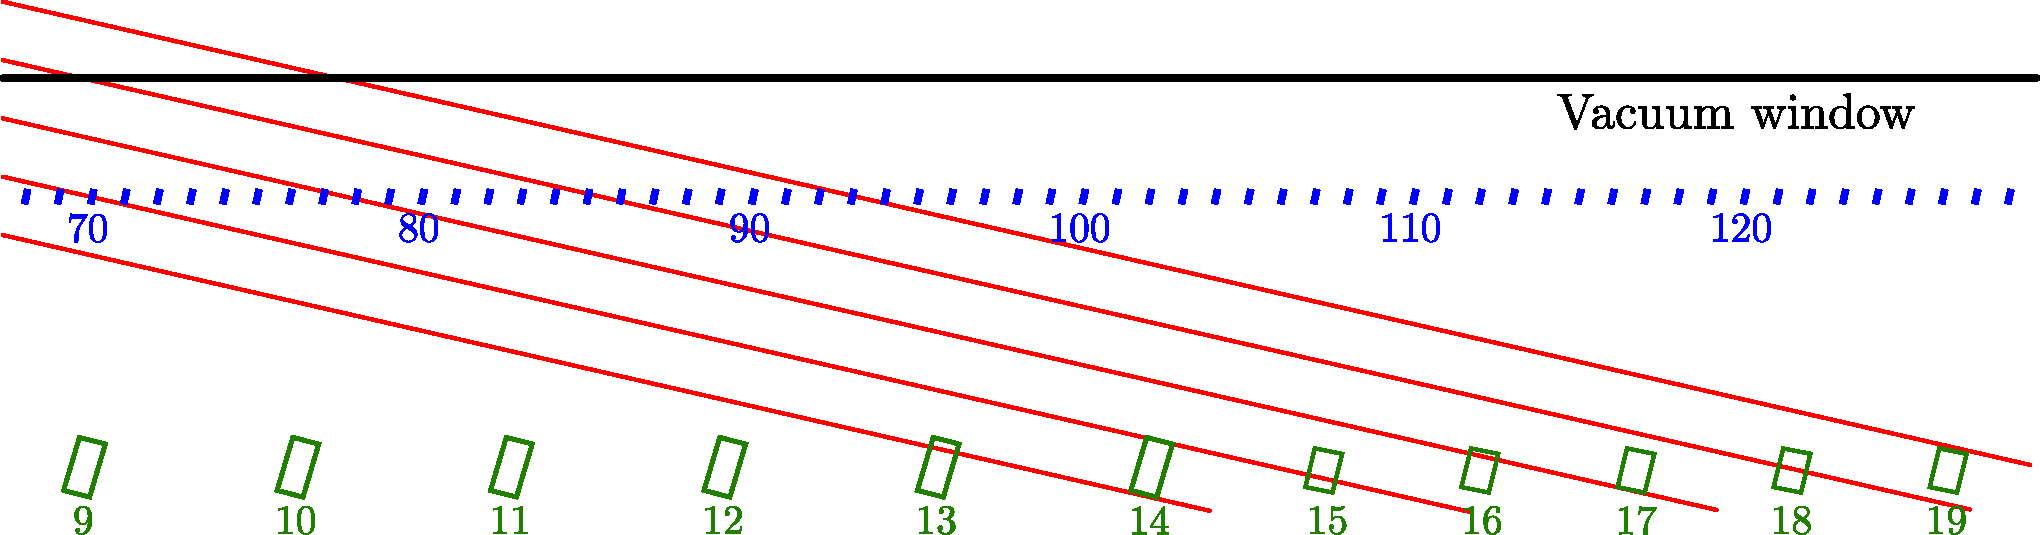
\includegraphics[width=1.1\figwidth,height=\qfigheight]{\grpath/hall-b/tagger_paddles.pdf}
\caption[Scale drawing of the $E$-counters (blue) and the $T$-counters (green) showing examples of recoiled electrons (red lines) entering from the upper left]{\label{fig:jlab.tagr.paddles}{\coloronline}Scale drawing of the $E$-counters (blue) and the $T$-counters (green) showing examples of recoiled electrons (red lines) entering from the upper left.}
\end{center}\end{figure}
\FloatBarrier

\section{CEBAF Large Acceptance Spectrometer (CLAS)} \label{sec:tjnaf.clas}

The \abbr{CLAS} detector, shown in Figs.~\ref{fig:clas}, ~\ref{fig:clas.ced}, is assembled of four types of detectors, five detectors total,  that are arranged in an onion like pattern (around the beam line) covering $\sim 3\pi$ with a diameter of 8~m. Each layer is segmented such that there are six segments around $\phi$ (angle about the beam line), called sectors, each with a polar coverage, $\theta$ (angle from beam line), of approximately $\frac{3}{4}\pi$~radians. Each sector consists of a scintillator start counter (\abbr{ST}) Sec.~\ref{sec:clas.st}, three layers of drift chambers (\abbr{DC}) Sec.~\ref{sec:clas.dc}, a layer of scintillator ``time-of-flight'' counters (\abbr{TOF}) Sec.~\ref{sec:clas.tof}, a gas Cherenkov counter (\abbr{CC}) Sec.~\ref{sec:clas.cc} and an electromagnetic calorimeter (\abbr{EC}) Sec.~\ref{sec:clas.ec}. There is a toroidal magnetic field generated by six superconducting coils that divide the sectors. The direction of the toroidal field is azimuthal, $\phi$ (angle about the beam line), such that the charged particles conserve their azimuthal angle along their trajectory, except near the coils. The magnetic field geometry guides the particles which allows for a simplified reconstruction algorithm to determine the particles' momenta, see Eq.~\ref{eq:motioninmag}. This section will discuss the subsystems in more detail.
% This field however produces an asymmetry in the acceptance of oppositely charged particles. 


\begin{figure}\begin{center}
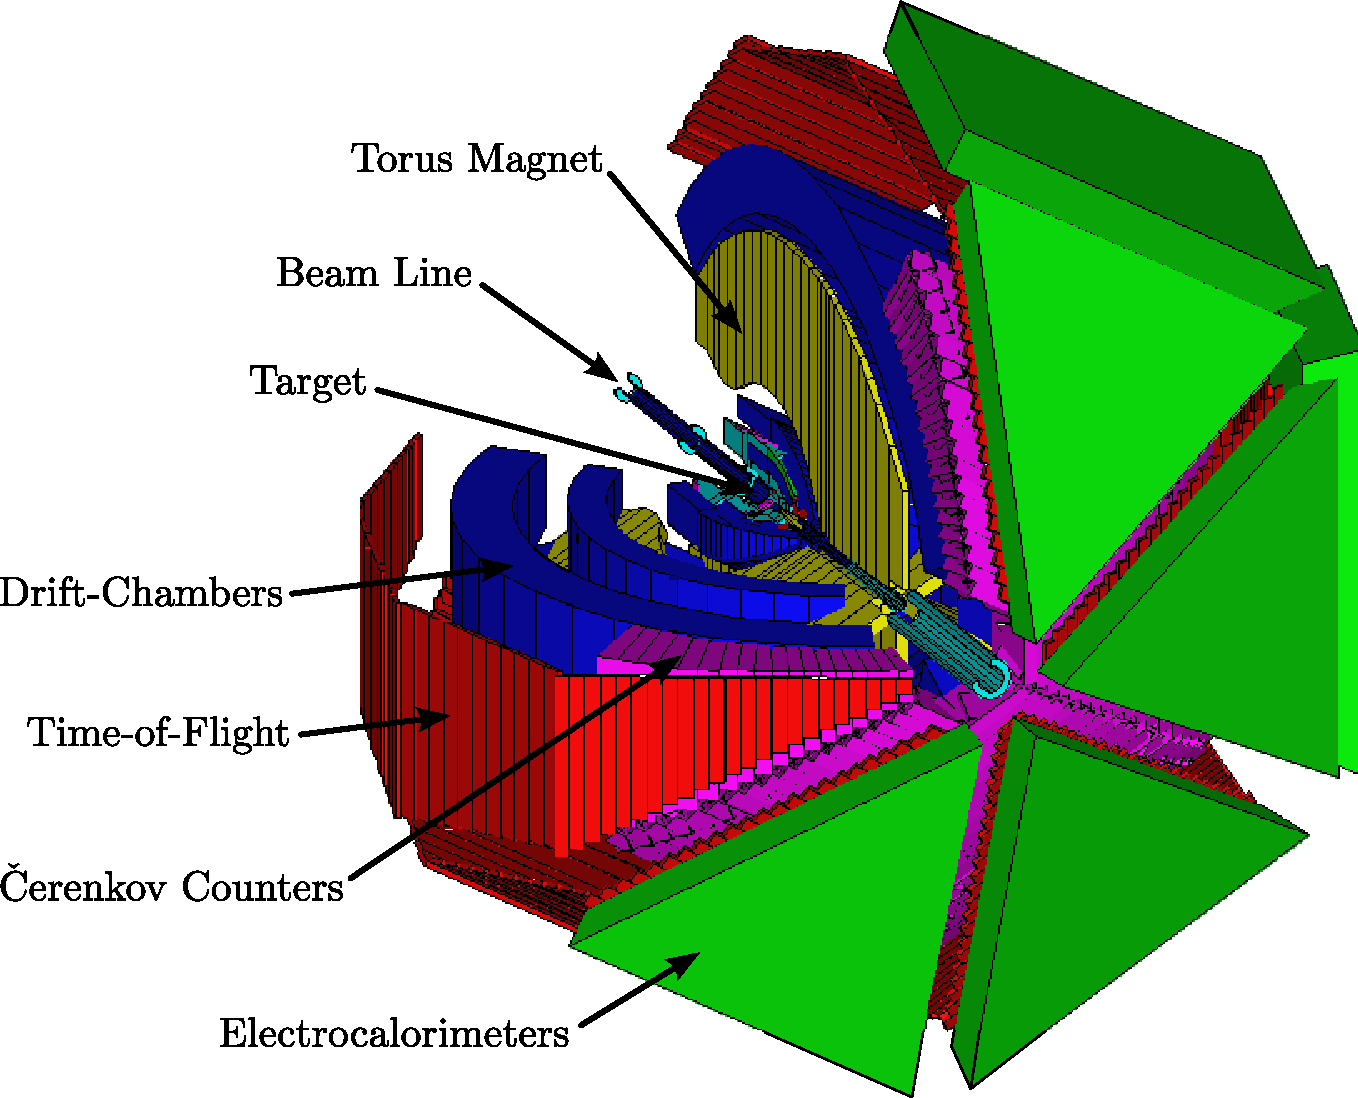
\includegraphics[width=0.8\columnwidth,height=0.75 \hfigheight]{\grpath/hall-b/clas_schematic.pdf}
\caption[Schematic of the \abbr{CLAS} detector with subsystems identified]{\label{fig:clas}{\coloronline}Schematic of the \abbr{CLAS} detector\cite{clas} with subsystems identified. This view is looking upstream and the beam enters from the upper left. The detector is approximately 8~meters in diameter.}
\end{center}\end{figure}

\begin{figure}\begin{center}
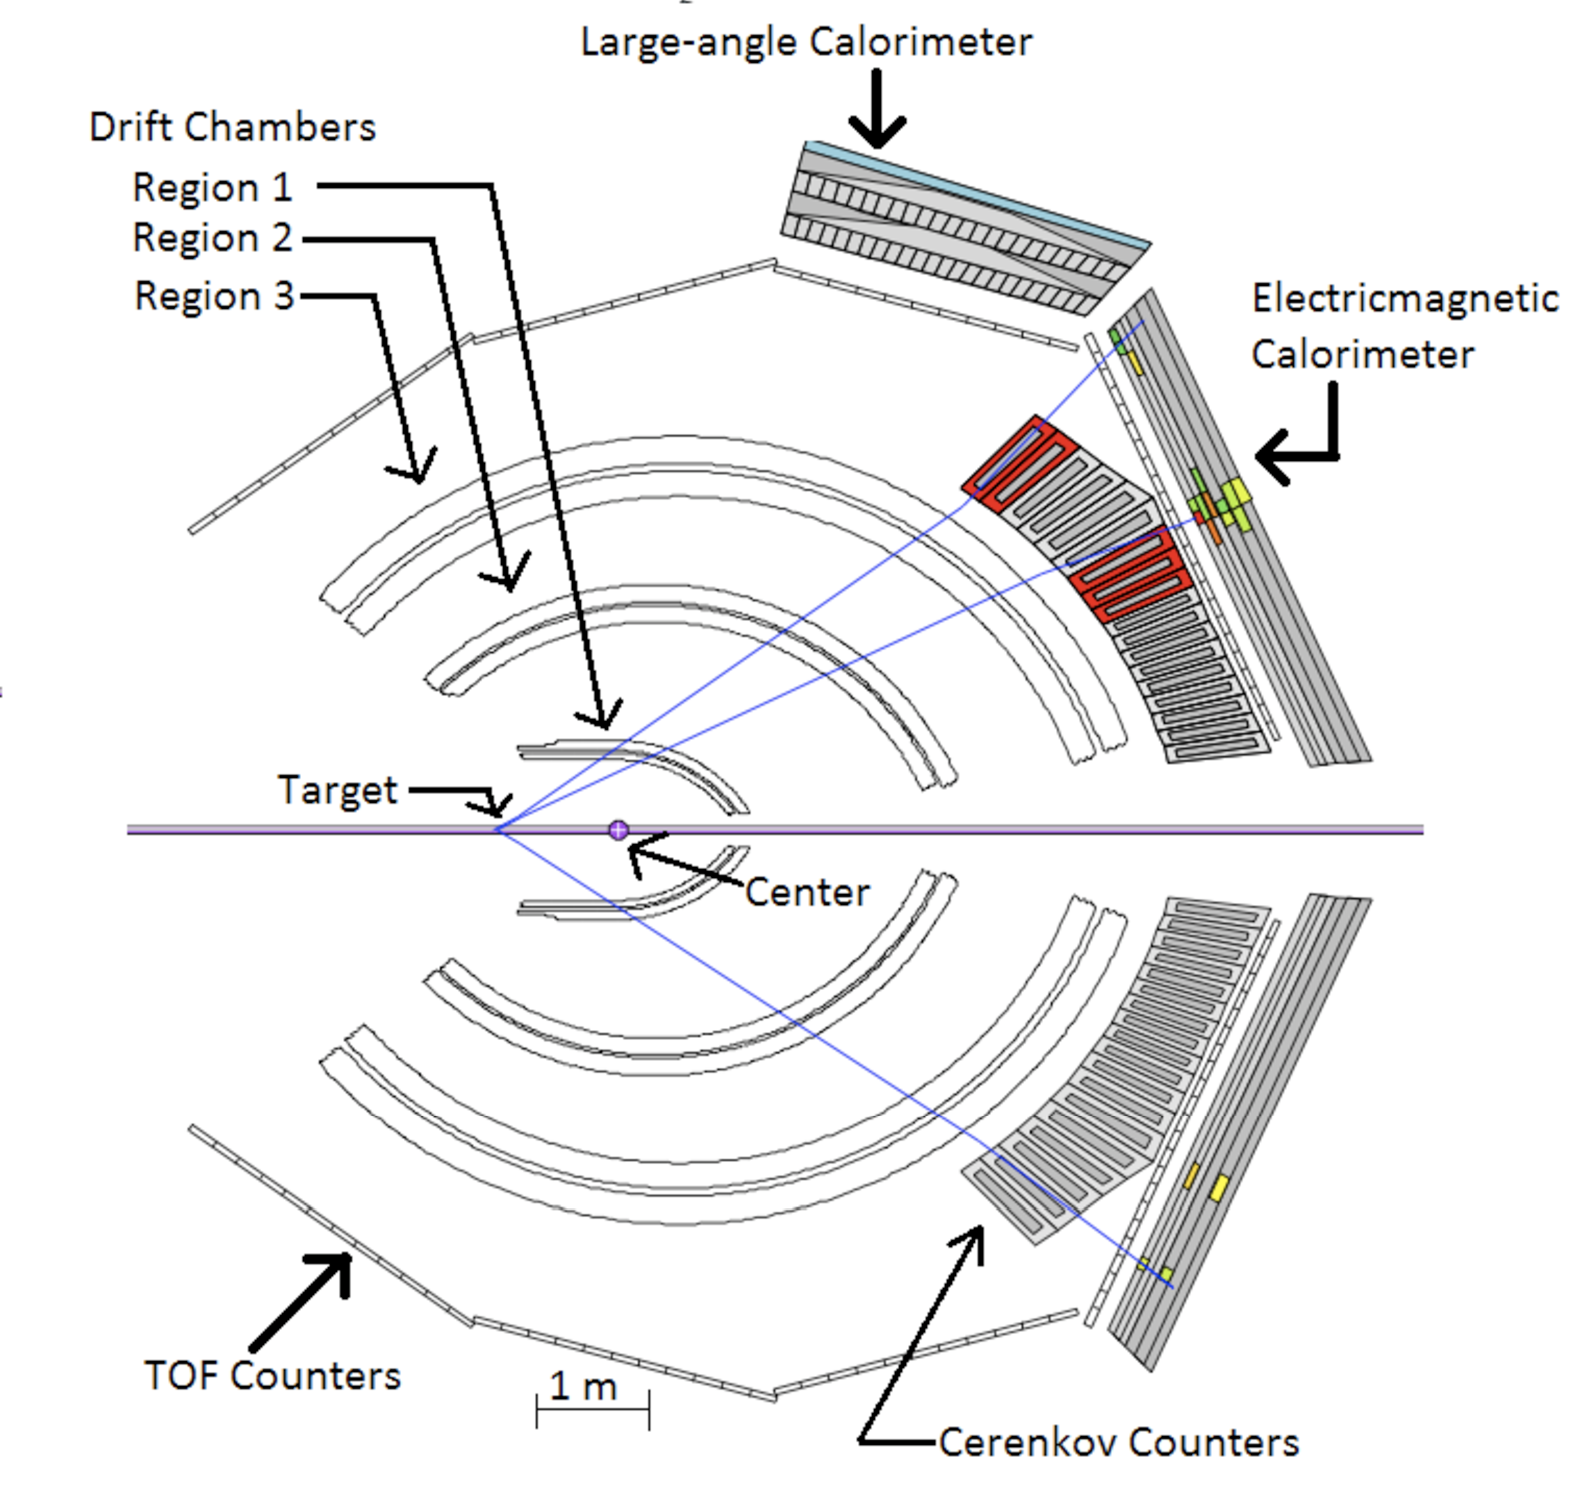
\includegraphics[width=0.6\columnwidth,height=0.75 \hfigheight]{\grpath/hall-b/clas_D.pdf}
\caption[A cross section view of the \abbr{CLAS} detector showing an event with three tracks emanating from the target]{\label{fig:clas.ced}A cross section view of the \abbr{CLAS} detector showing an event with three tracks emanating from the target. The two tracks leaving hit patterns \abbr{CC} and \abbr{EC} are leptons while the track on the bottom panel is a proton}
\end{center}\end{figure}

\begin{figure}\begin{center}
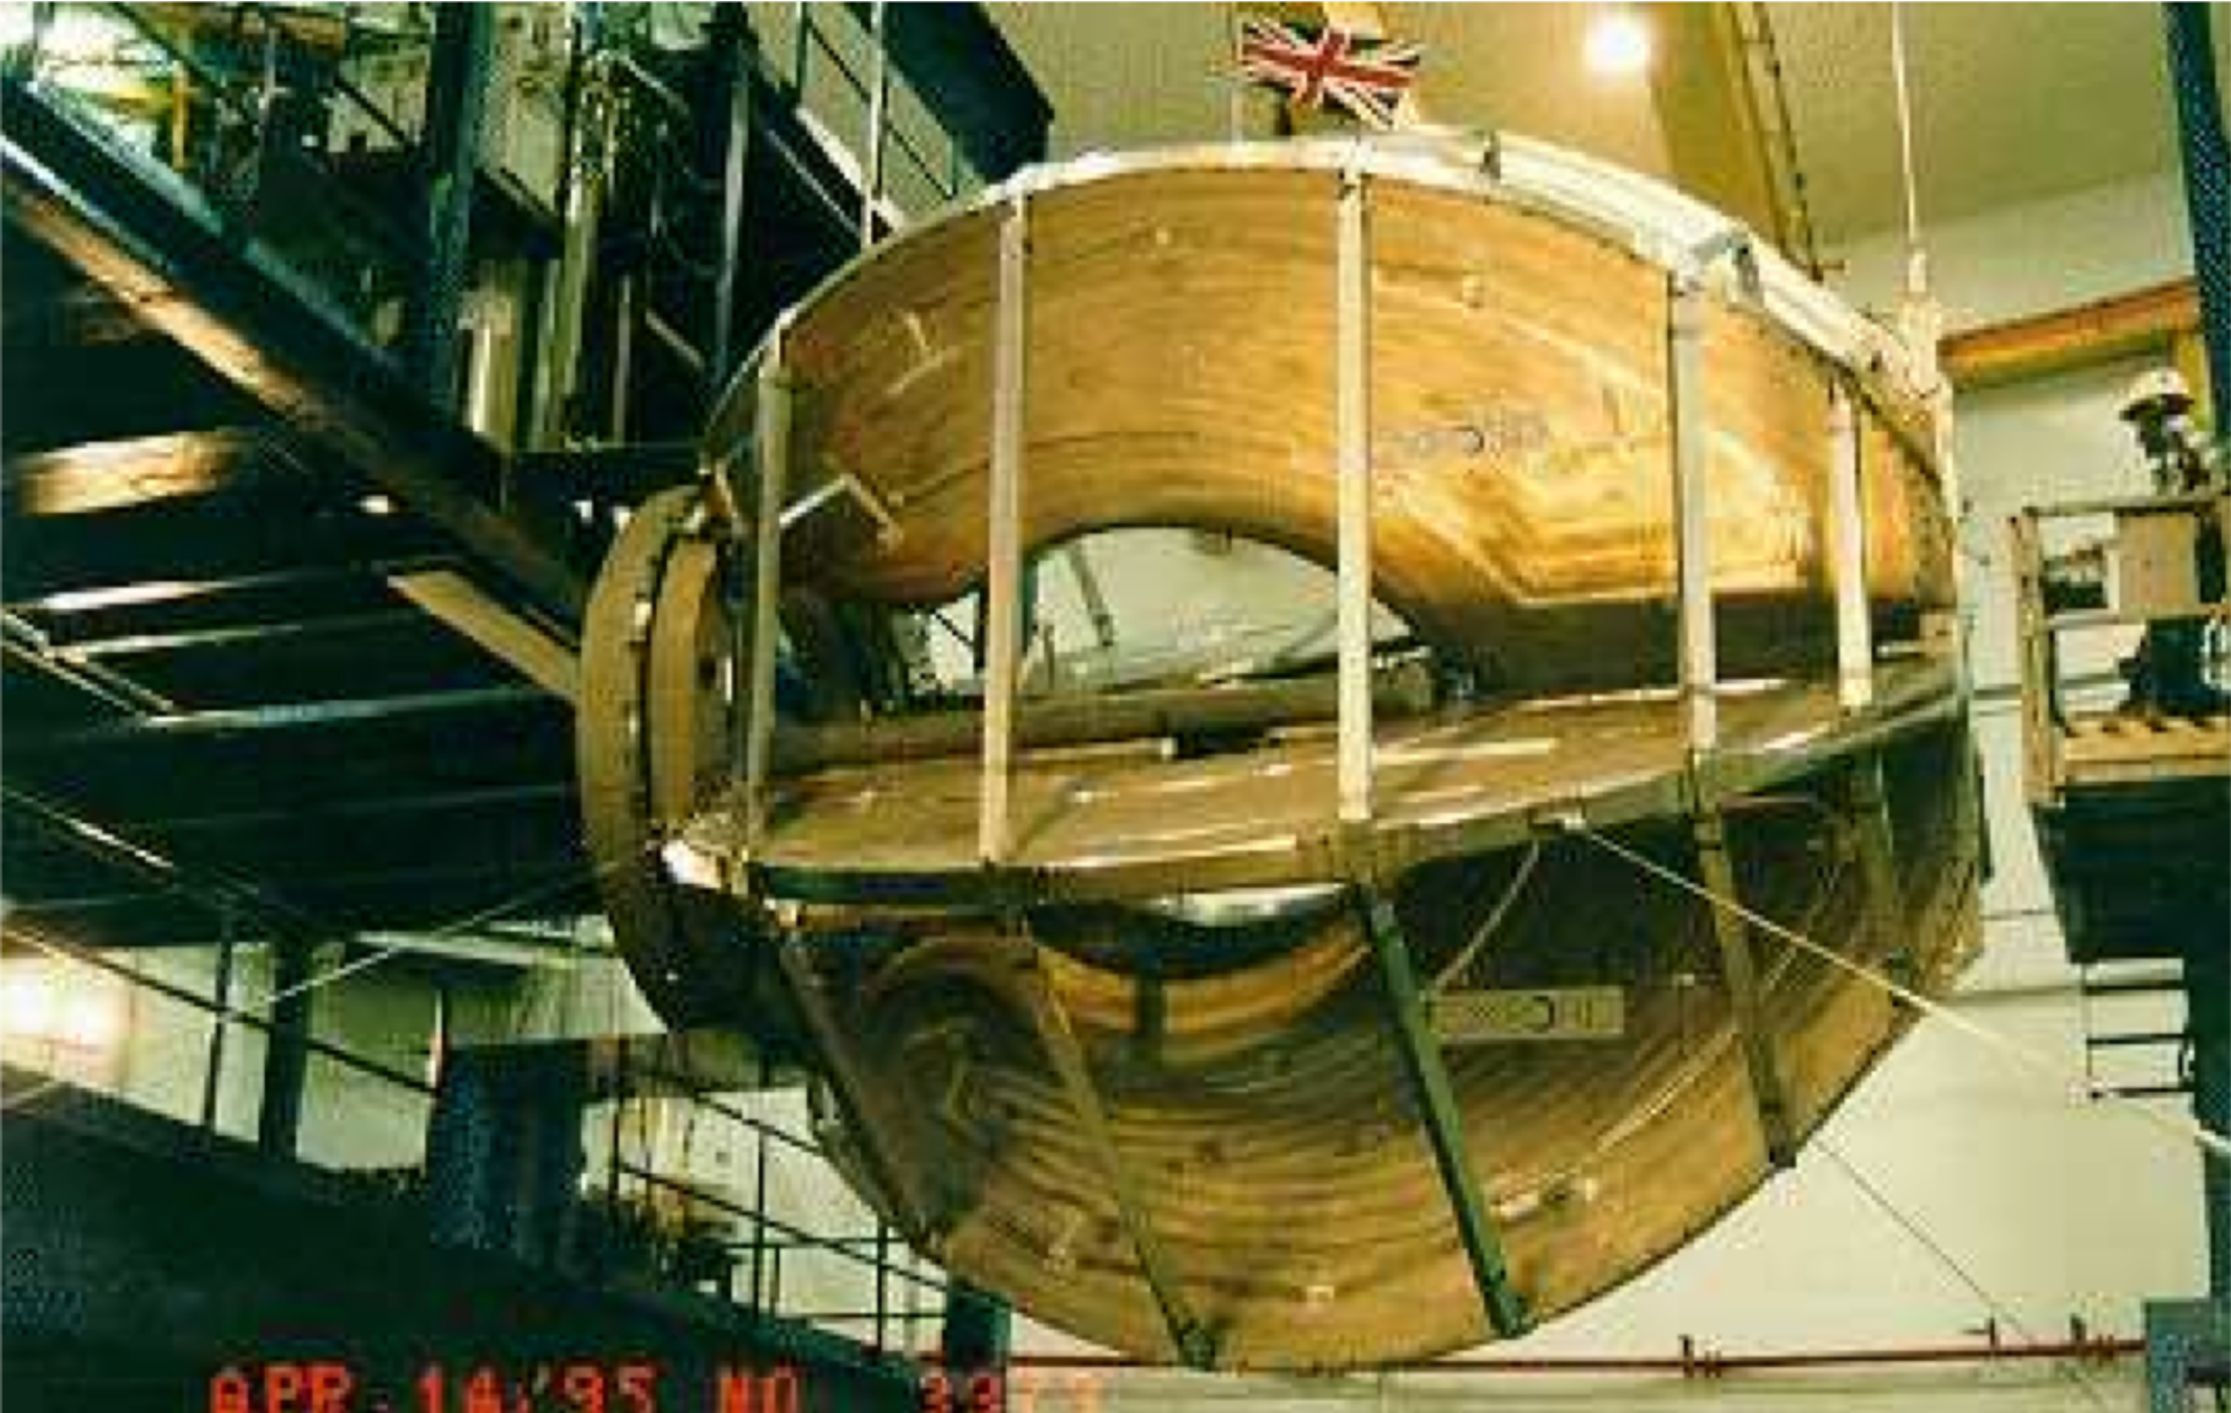
\includegraphics[width=0.55\columnwidth,height=\qfigheight]{\grpath/hall-b/torus_install.pdf}
\caption[The coils of the \abbr{CLAS} toroidal magnet prior to installation of the rest of the detector]{\label{fig:torusinstall}{\coloronline}The coils of the \abbr{CLAS} toroidal magnet prior to installation of the rest of the detector. Image Source~\cite{williams}}
\end{center}\end{figure}
\FloatBarrier

\subsection{Hydrogen Cryotarget}\label{sec:clas.tgt}


The target used by \g12 was conical as shown in Fig.~\ref{fig:clas.targetblueprint}. The target walls were constructed of 0.127~$\mu$m thick Kapton. It is 40~cm in length and 2~cm in radius. The incident photon beam had a radius of 1.5~cm. The target cell design shown in Figs,~\ref{fig:clas.targetblueprint} and~\ref{fig:clas.targetcell} had been used in several experiments and is capable of containing a number of different materials, such as helium, deuterium and hydrogen. For \g12 the target was filled with liquid hydrogen ($\ell$H$_2$). The temperature and pressure of the target was continuously measured and recorded. In Sec~\ref{sec:analysis.target_density}, these measurements will be used to calculate the density of the liquid Hydrogen to determine the target thickness. The target was not polarized.

\begin{figure}[h!]\begin{center}
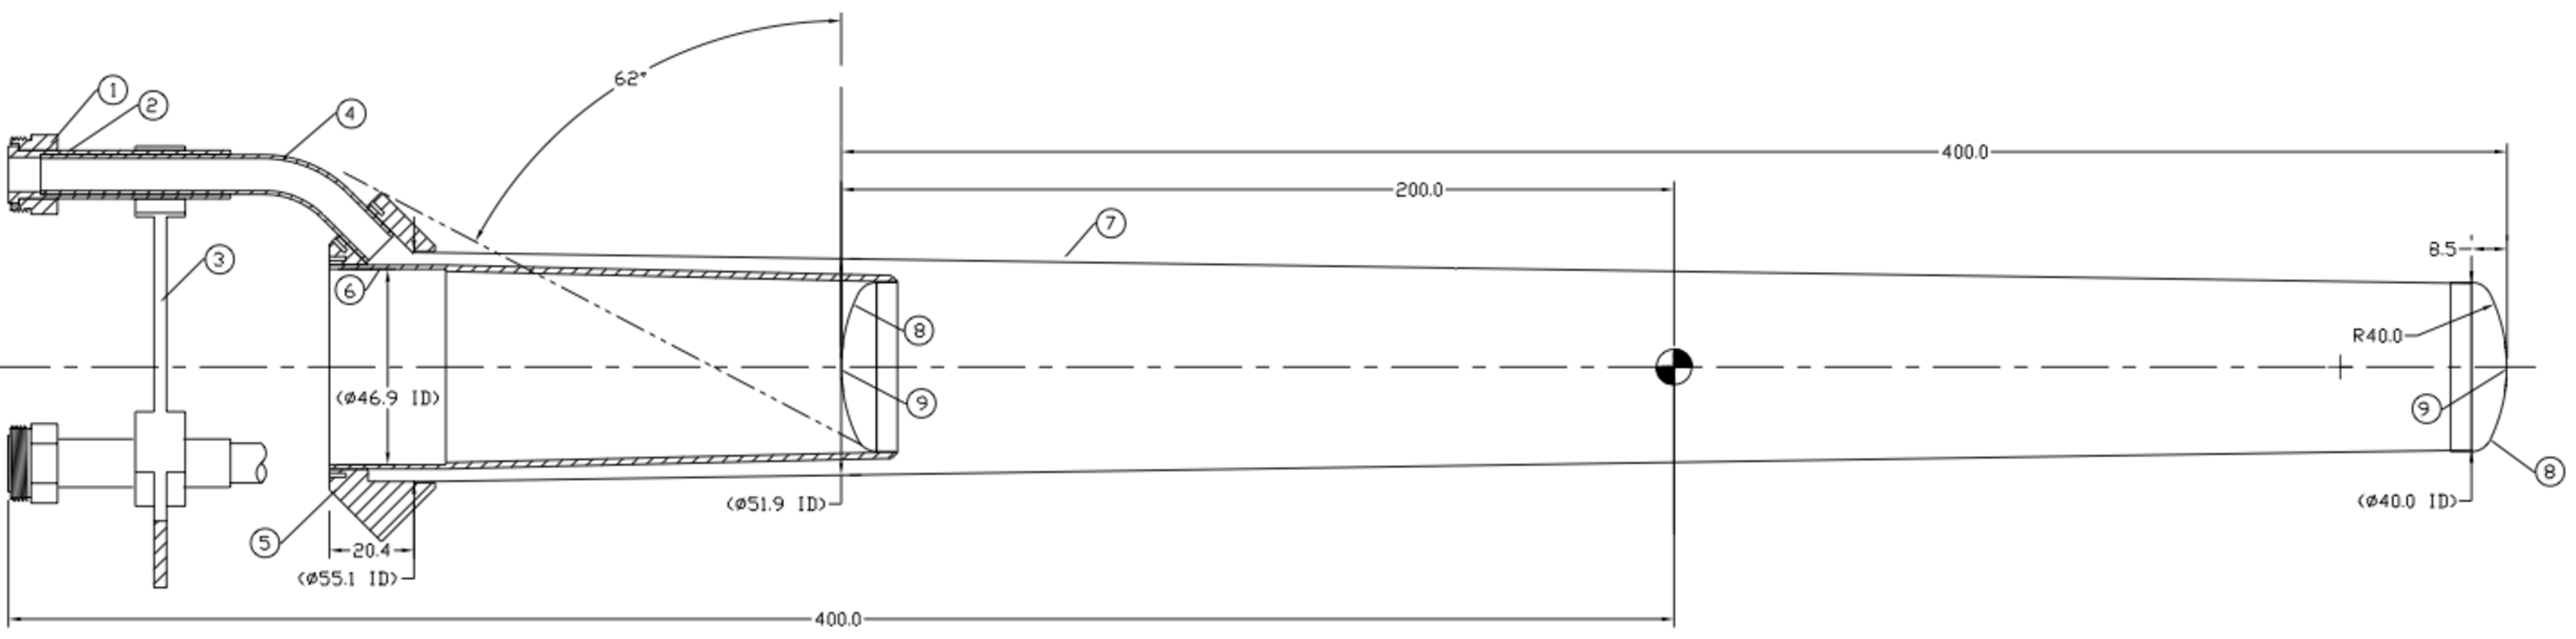
\includegraphics[width=\figwidth,height = \qfigheight]{\grpath/hall-b/g11_target_cell_blueprint.pdf}
\caption[Blueprint schematic of the conical Kapton target cell used for \g12]{\label{fig:clas.targetblueprint}Blueprint schematic of the conical Kapton target cell used for \g12.}
\end{center}\end{figure}

\begin{figure}[h!]\begin{center}
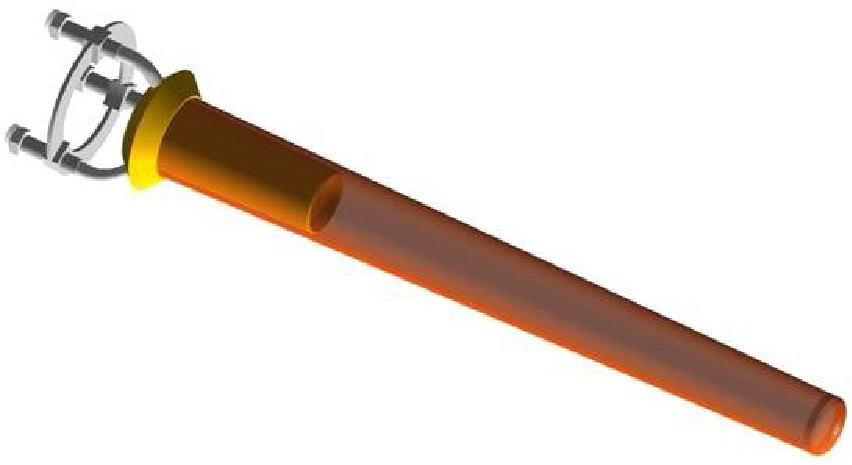
\includegraphics[width=0.6\figwidth]{\grpath/hall-b/g11_target_cell.pdf}
\caption[The 40~cm long conical Kapton target cell used for \g12]{\label{fig:clas.targetcell}The 40~cm long conical Kapton target cell used for \g12.}
\end{center}\end{figure}

%\subsubsection{Target Position for \g12}\label{sec:clas.tgt.position}
The target was located 90~cm upstream of \abbr{CLAS} the center, see Fig.~\ref{fig:clas.ced}.
This increased the forward angle acceptance from 8$^\circ$  to 6$^\circ$. However, this also decreased the large angle acceptance from approximately 140$^\circ$ to 100$^\circ$ in the lab frame.
%This reduction in large angle acceptance sacrificed multi-particle final state events, where the final state particles were more than about 70$^\circ$ away from beamline.
%as well as a reduction in \abbr{DC} resolution. The \abbr{DC} resolution decrease was due to the oblique angle the tracks made with the detector planes.
\FloatBarrier
\section{Start Counter}\label{sec:clas.st}

The start counter, Figs.~\ref{fig:clas.st} and~\ref{fig:clas.stxsection}, is a \abbr{PMT}-instrumented scintillator detector that surrounds the CLAS cryotarget hermetically. It consists of 24 scintillation paddles divided into six sectors matching that of \abbr{CLAS}. Each sector of the start counter is constructed of four independently-instrumented scintillator strips. Timing resolution of the start counter is $\sim$350~ps. The start counter information was used the \g12 triggers~\ref{sec.data.trig.lepton}. More information on the CLAS start counter can be found in \cite{clas.st}.

\begin{figure}[h!]\begin{center}
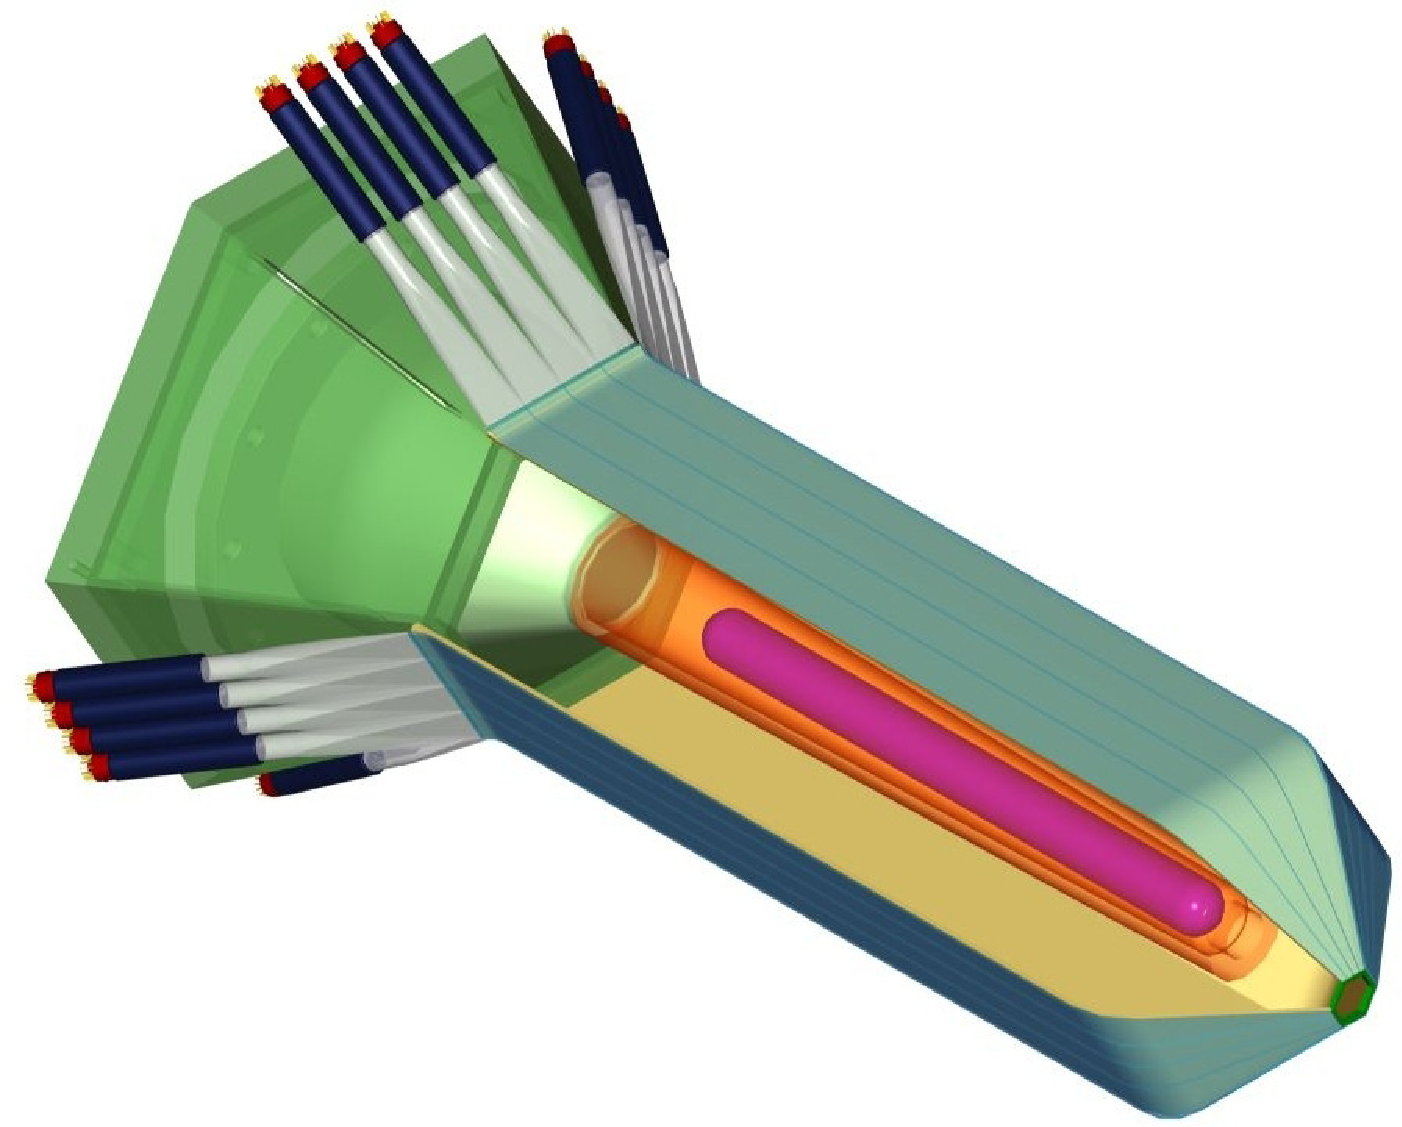
\includegraphics[width=0.8\figwidth,height=\qfigheight]{\grpath/hall-b/start_counter.pdf}
\caption[Schematic of the start counter (\abbr{ST}) with the 40~cm long target cell (purple) at the center]{\label{fig:clas.st}{\coloronline}Schematic of the start counter (\abbr{ST}) with the 40~cm long target cell (purple) at the center. The beam enters from the upper left of the figure.}
\end{center}\end{figure}

\begin{figure}[h!]\begin{center}
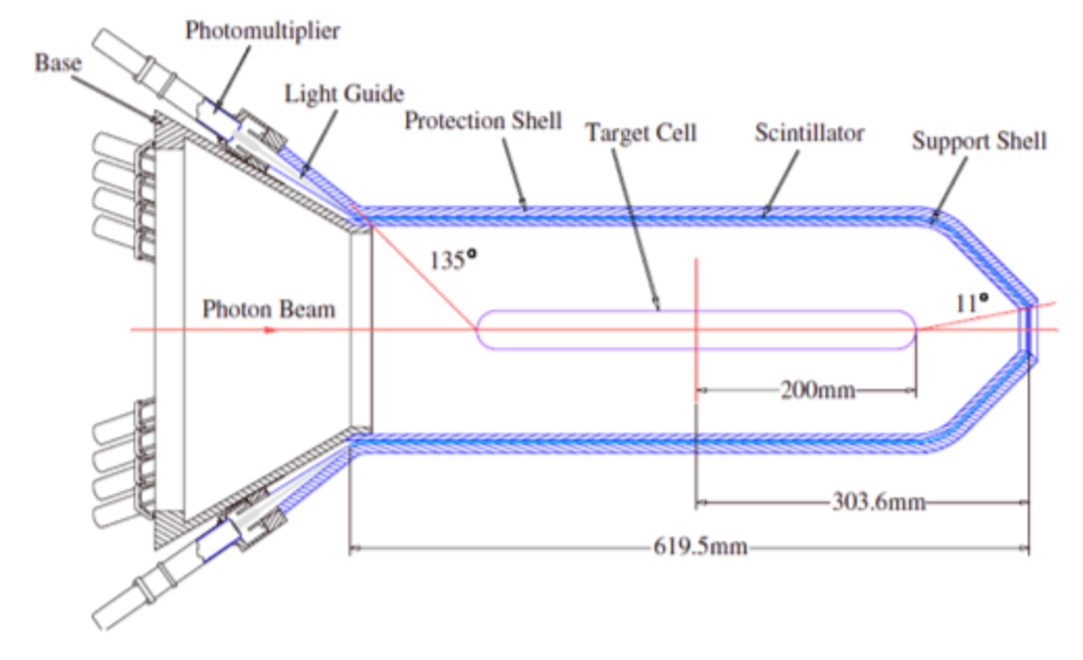
\includegraphics[width=0.8\figwidth,height=\qfigheight]{\grpath/hall-b/start_counter_wtarget.pdf}
\caption[Cross-section view of the start counter illustrating the labeled components and its angular coverage when at the center of \abbr{CLAS}]{\label{fig:clas.stxsection}{\coloronline}Cross-section view of the start counter illustrating the labeled components and its angular coverage when at the center of \abbr{CLAS}.}
\end{center}\end{figure}

\FloatBarrier
%\subsection{Start Counter Efficiency Analysis}\label{sec:clas.st.eff}
%There is an inefficiency of the start counter as seen in Fig.~\ref{fig:classt.ineff}. This inefficiency was measured by using real data events as generated events and passing them through \abbr{CLAS}'s Monete-Carlo package(\abbr{GSIM}\label{abbr:gsim}). More information about this inefficiency will be discussed in Sec.~\ref{sec:analysis.accept.verify}.
%
%%It was observed that 20~\% of the events would fail in simulation, this will be discussed in Sec~\ref{sec:gsim.efficiency}. A portion of the failed events were based upon a failure to reconstruct the required banks for the start counter. This phenomena was investigated from the raw data and found to also be present in the processing of the data from raw to user file in the same manner as seen from Monte-Carlo. The blue-dashed line in Fig.~\ref{fig:classt.ineff} illustrates the start counter inefficiency that is dependent on the events reconstructed vertex. The inefficiency is due to the start counter reconstruction algorithm not being able to link the start counter hit to a track through time-based tracking. This track is not lost due to a reprocess of time-based tracking, linking the track to another particles start counter hit with the same 
%
%%The inefficiency of the start counter is not a mechanical fault but rather the fault of the algorithm used to reconstruct a start counter hit. TO study this raw data events were processed event by event using the program DDD and \abbr{CLAS} event display (\abbr{ced}). Unknown of the cause, it  
%
%
%\begin{figure}[h!]\begin{center}
%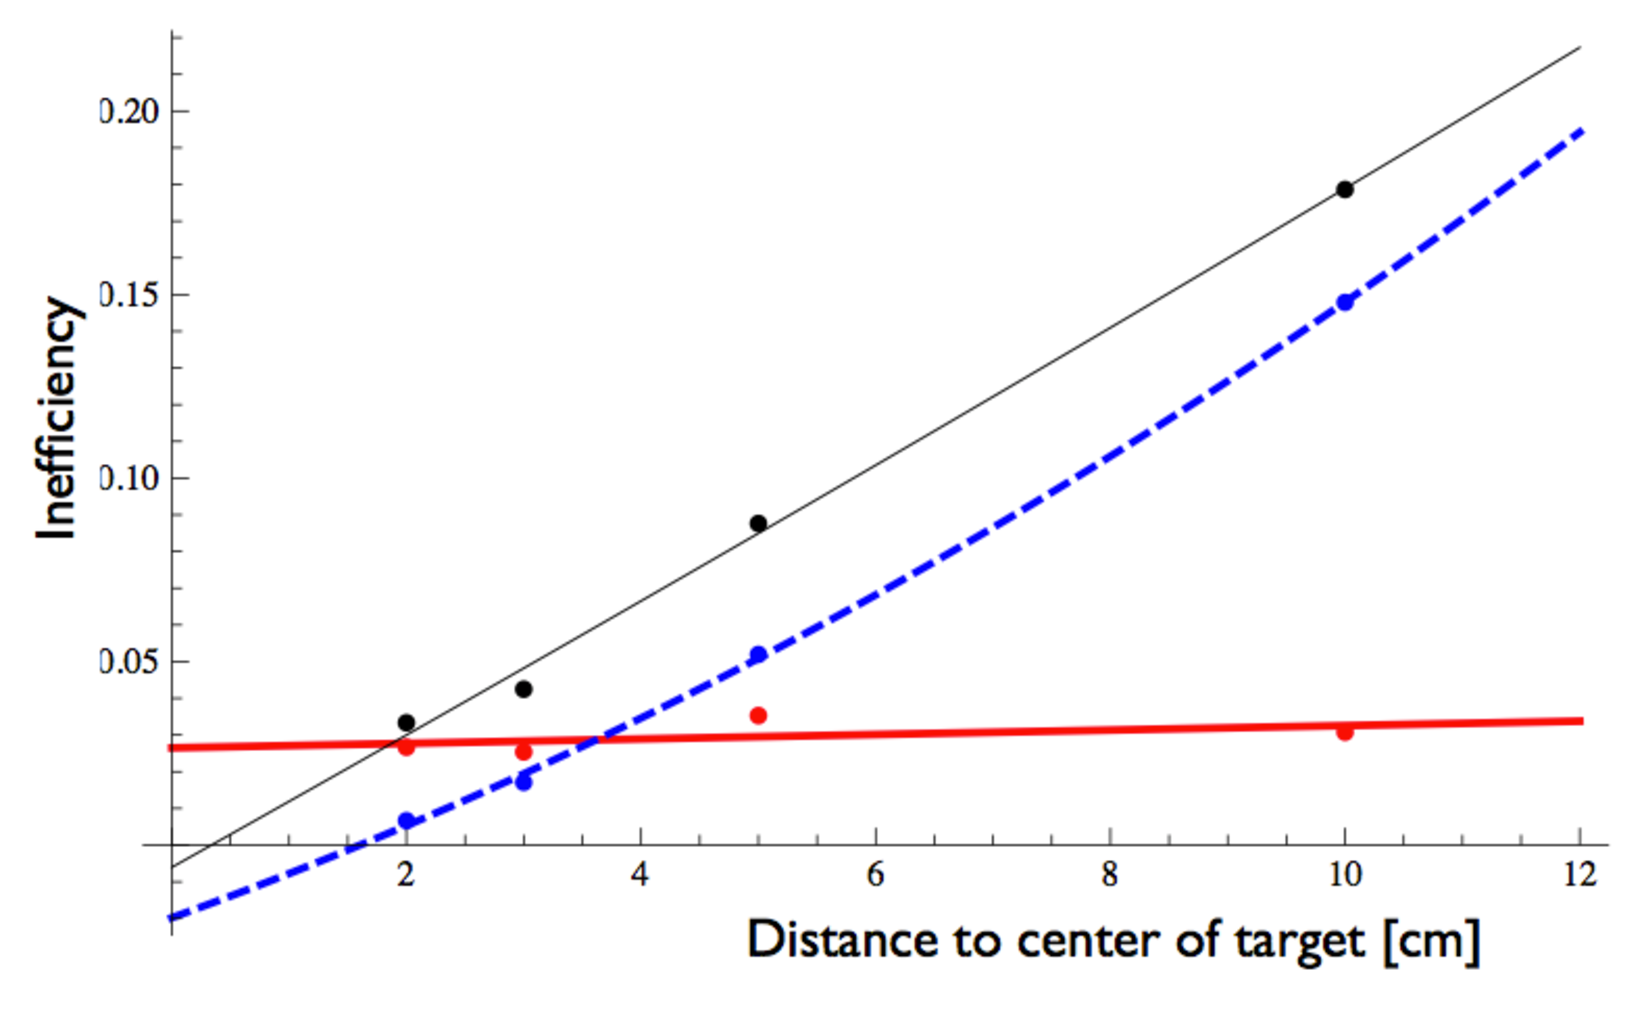
\includegraphics[width=0.8\figwidth,height=0.7\hfigheight]{\grpath/hall-b/st_issue_4_thesis.pdf}
%\caption[Start Counter Inefficiency]{\label{fig:classt.ineff}{\coloronline}Plot showing the inefficiency of the start counter from data events, red-solid line is the inefficiency of reconstruction based solely on hit-based tracking, blue-dashed line is inefficiency of start counter, black-solid is combined. }
%\end{center}\end{figure}
%
%\FloatBarrier
\section{Superconducting Toroidal Magnet}\label{sec:clas.tor}

The essence of \abbr{CLAS} is the use of a toroidal magnetic field generated by six superconducting coils consisting of 4 layers of 54 windings of aluminum-stabilized niobium titanium NbTi/Cu superconductor \cite{clas}. The coils are separated in the azimuthal direction, $\phi$, by 60$^\circ$ and are located between Region-1 and Region-3 of the \abbr{DC}, see Fig~\ref{fig:clas.dc.torus.mag}. The placement of the coils is such that the magnetic field is encompassed by the volume of the \abbr{DC}, see Fig.~\ref{fig:clas.dc.torus.mag}. The direction of the toroidal field points along $\phi$, except near the coils,  such that the charged particles conserve their azimuthal angle along their trajectory, see Fig~\ref{fig:clas.dc.torus.cont}. The maximum current the magnet can support is 3861~A, resulting in a maximum field strength of 35~kG. During the \g12 experiment, the magnets operated at a current of 1930~A corresponding to a maximum field of about 20~kG. The field was oriented such that positive charged particles bent away from the beam-line, while negative charged particles bent toward the beam-line. Running at higher currents provides better momentum resolution but decreases the detector's acceptance for negative particles. Knowing the strength and direction of the magnetic field and the trajectory of a particle using the \abbr{DC}, the particle momentum can be determined by use of Eq.~\ref{eq:motioninmag}.
% During the \g12 experiment, the magnet was cooled down to 4.5~K using liquid helium ($\ell$He) obtained from the central CEBAF central cryogenic facility.

\begin{figure}[h!]\begin{center}
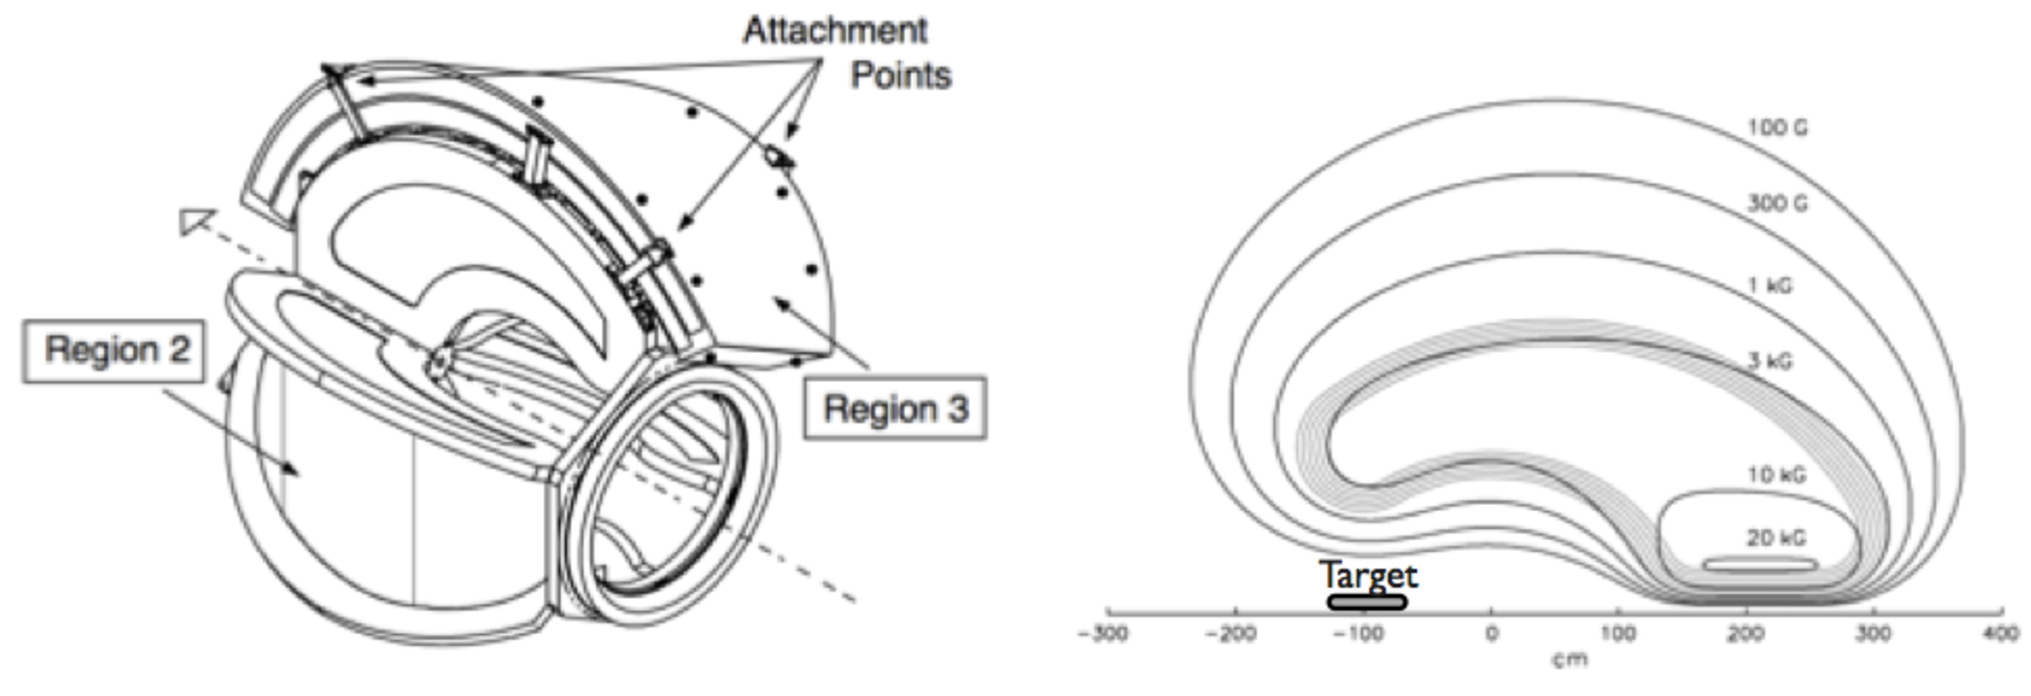
\includegraphics[width=\figwidth,height=0.9\qfigheight]{\figures/hall-b/torus_field_mag_mount.pdf}
\caption[The \abbr{CLAS} Superconducting Toroidal Magnet and its placement in relation to Region-1 and Region-3]{\label{fig:clas.dc.torus.mag}The \abbr{CLAS} Superconducting Toroidal Magnet and its placement in relation to Region-1 and Region-3  (left). Cross-section of the \abbr{CLAS} Superconducting Toroidal Magnet at half current (1930~A). Region-2 of the \abbr{DC} is located inside the region of the coils shown as the kidney shaped loop at about 3~kG (right).}
\end{center}\end{figure}

\begin{figure}[h!]\begin{center}
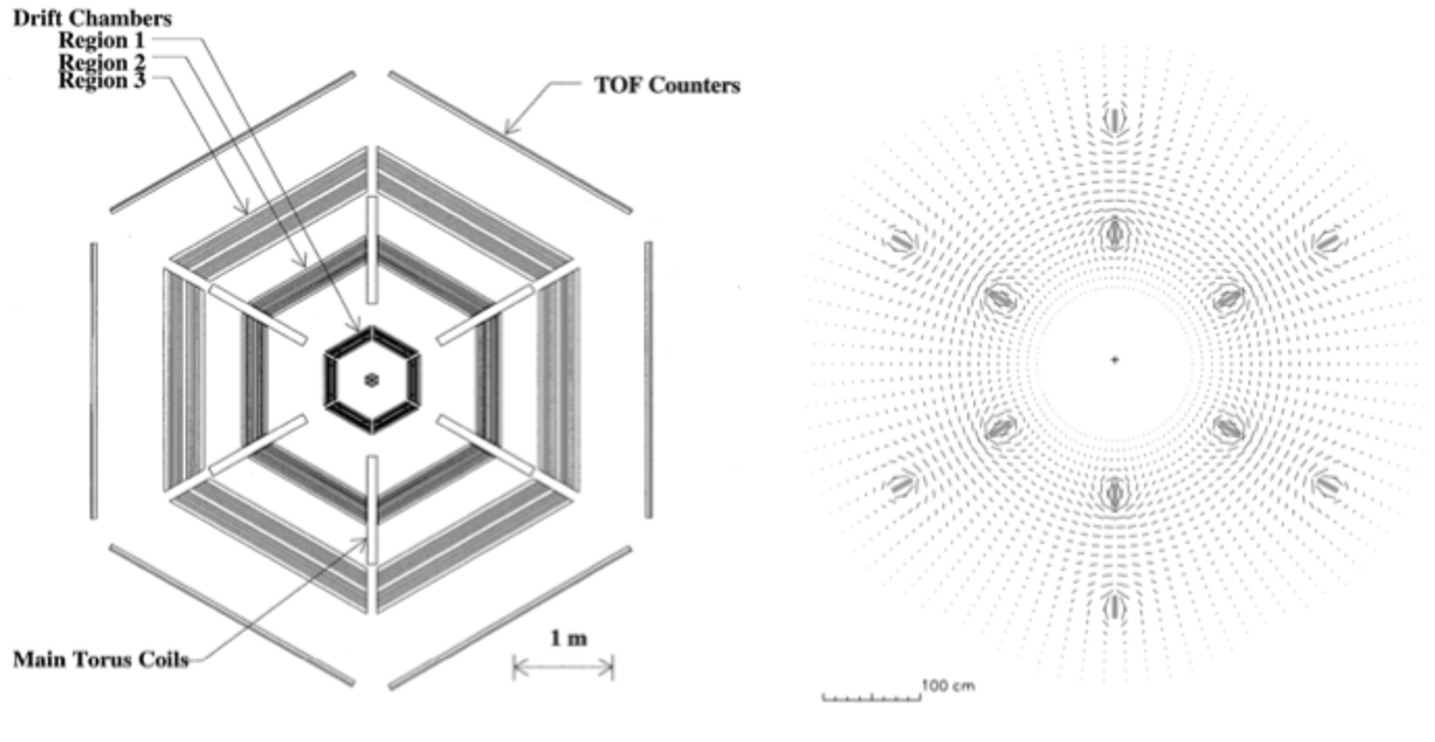
\includegraphics[width=1.\figwidth,height=0.75\hfigheight]{\figures/hall-b/torus_field_and_DC.pdf}
\caption[Schematic cross-sectional view of the \abbr{CLAS} detector, perpendicular to the beam line]{\label{fig:clas.dc.torus.cont}Schematic cross-sectional view of the \abbr{CLAS} detector, perpendicular to the beam line (left). The magnetic field distribution corresponding to the view in the left figure. The field is purely azimuthal. The six torus coils are shown in grey, the field is in the counter-clockwise direction,  the field strength is concentrated in the region between the coils (right).}
\end{center}\end{figure}

\FloatBarrier
\section{Drift Chambers}\label{sec:clas.dc}

The \abbr{CLAS} drift chambers \abbr{DC} (Figs.~\ref{fig:clas},~\ref{fig:clas.dc.torus.cont},~\ref{fig:clas.dc.drift}) track charged particles above 200~MeV/c with polar angle resolution of 2-4~mrad and momentum resolution of 0.5 - 1\%, depending on momentum, see Fig~\ref{fig:clas.dc.res}. Typical coverage of the \abbr{DC} is $8^\circ < \theta < 142^\circ$, when the target is at \abbr{CLAS} center. For the \g12 experiment the coverage of the \abbr{DC} was modified to $6^\circ < \theta < 100^\circ$ due to the placement of the target, see Sec~\ref{sec:clas.tgt} for reasons explained in ~\cite{clas.proposal.hyclas},~\cite{clas.proposal.superg},~\cite{clas.proposal.pion}.
\begin{figure}\begin{center}
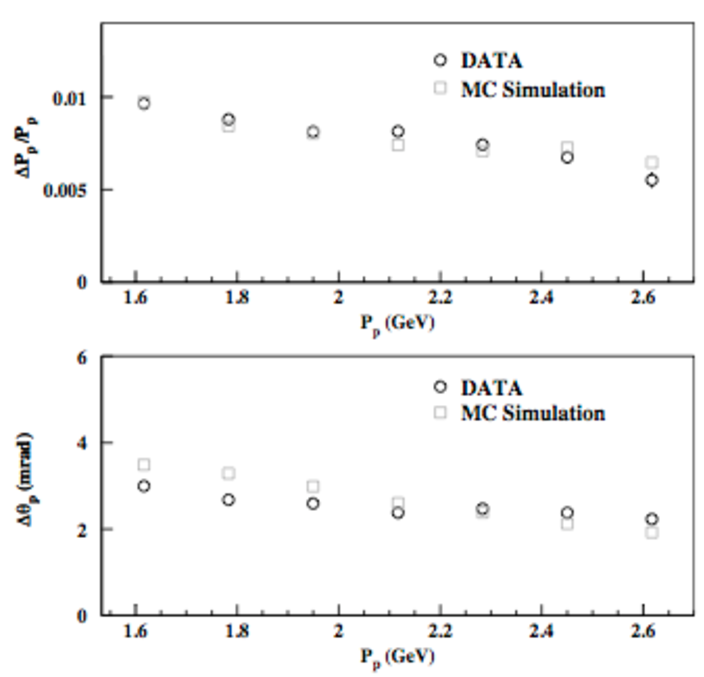
\includegraphics[width=0.8\figwidth,height=0.75\hfigheight]{\figures/hall-b/drift_DC_resolution.pdf}
\caption[Momentum and angular resolution for protons as determined from the measured angle of the scattered electron for data collected and Monte-Carlo simulation]{\label{fig:clas.dc.res}Momentum and angular resolution for protons as determined from the measured angle of the scattered electron for data collected and Monte-Carlo simulation. Image Source~\cite{clas}}
\end{center}\end{figure}

The \abbr{DC} are divided into six sectors each containing three radial layers (Fig.~\ref{fig:clas.dc.drift}), referred to as ``Regions'', for a total of 18 separate drift chambers. Each \abbr{DC} region covers the same polar angular range and consist of two superlayers which each contain six layers of hexagonal wire cells which house evenly spaced 20~$\mu$m gold-plated tungsten sense wires (center of hexagon) each surrounded by six 140~$\mu$m gold-plated aluminum alloy field wires (vertices of hexagon). In the first superlayer, the wires are strung approximately parallel to the direction of the magnetic field (axial wires), while the second superlayer has wires tilted at a 6$^\circ$ angle with respect to the axial wires (stereo wires). A high voltage system maintains the sense wires at positive potential, while the field wires are maintained at a negative potential 50\% lower than the positive value. The difference of potentials creates an avalanche of the electrons induced by the ionizing particle. The hexagonal shape of the cell mimics a circular geometry cell in which the drift time to drift distance is independent of entrance angle.

The inner region is denoted as Region 1. Its first superlayer has only 4 layers due to space constraints. Region 1 is nearly free from magnetic field, see Fig~\ref{fig:clas.dc.torus.mag}. Region 2 is situated between the magnetic coils which is subject to the highest magnetic field which is used to determine the particle's curvature, needed to determine the particle;s momenta, see Eq.~\ref{eq:motioninmag}. Region 3 purpose is to provide global track reconstruction in connection with other CLAS detectors since Region 3 is located outside the volume of magnetic field. Each \abbr{DC} is filled with a gas mixture of 90\% argon and 10\% carbon-dioxide. This choice of gas provides high drift velocity (0.04 m/$\mu$sec) and fast collection time which improves momentum resolution. For more information on the design of the \abbr{CLAS} \abbr{DC} system, see~\cite{clas.dc} and for more information on the calibration process of the \abbr{CLAS} \abbr{DC} system, see~\cite{clas.dc.calib}.

\begin{figure}\begin{center}
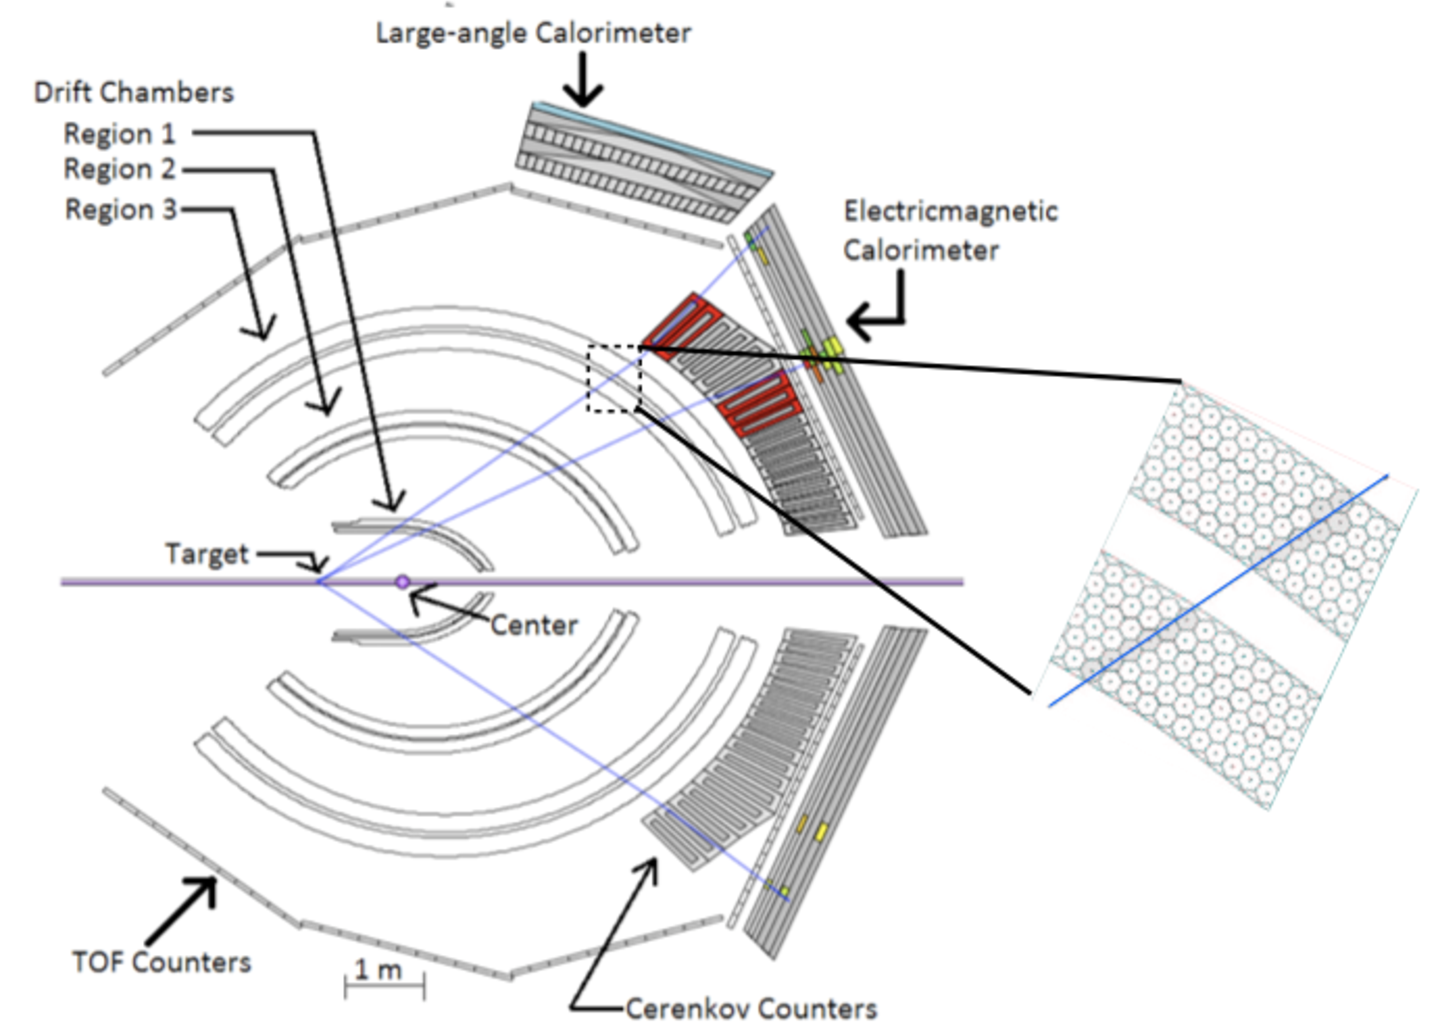
\includegraphics[width=\figwidth,height=0.75\hfigheight]{\figures/hall-b/drift_DC_cedII.pdf}
\caption[A cross section view of the \abbr{CLAS} detector showing an event with three tracks emanating from the target]{\label{fig:clas.dc.drift}A cross section view of the \abbr{CLAS} detector showing an event with three tracks emanating from the target. The two tracks leaving hit patterns \abbr{CC} and \abbr{EC} are leptons while the track on the bottom panel is a proton. The inlet shows hexagonal cells of drift chambers with a typical track indicated by shaded areas for the cut-out in Region-3.}
\end{center}\end{figure}

\FloatBarrier
\section{Cherenkov Radiation and Detectors}\label{sec:clas.cc}

When a charged particle traverses through a medium with a velocity less than the speed of light for that medium ($v < c/n$) the dipoles of the molecules in the medium are symmetrically arranged such that the integrated dipole field along the particles path vanishes. However, when the particles speed is greater than that of the speed of light for that medium the dipoles of the molecules arrange themselves such that they are asymmetric along the particles path and thus creates a dipole field, see Fig~\ref{fig:clas.cc.dipole}.
\begin{figure}[h!]\begin{center}
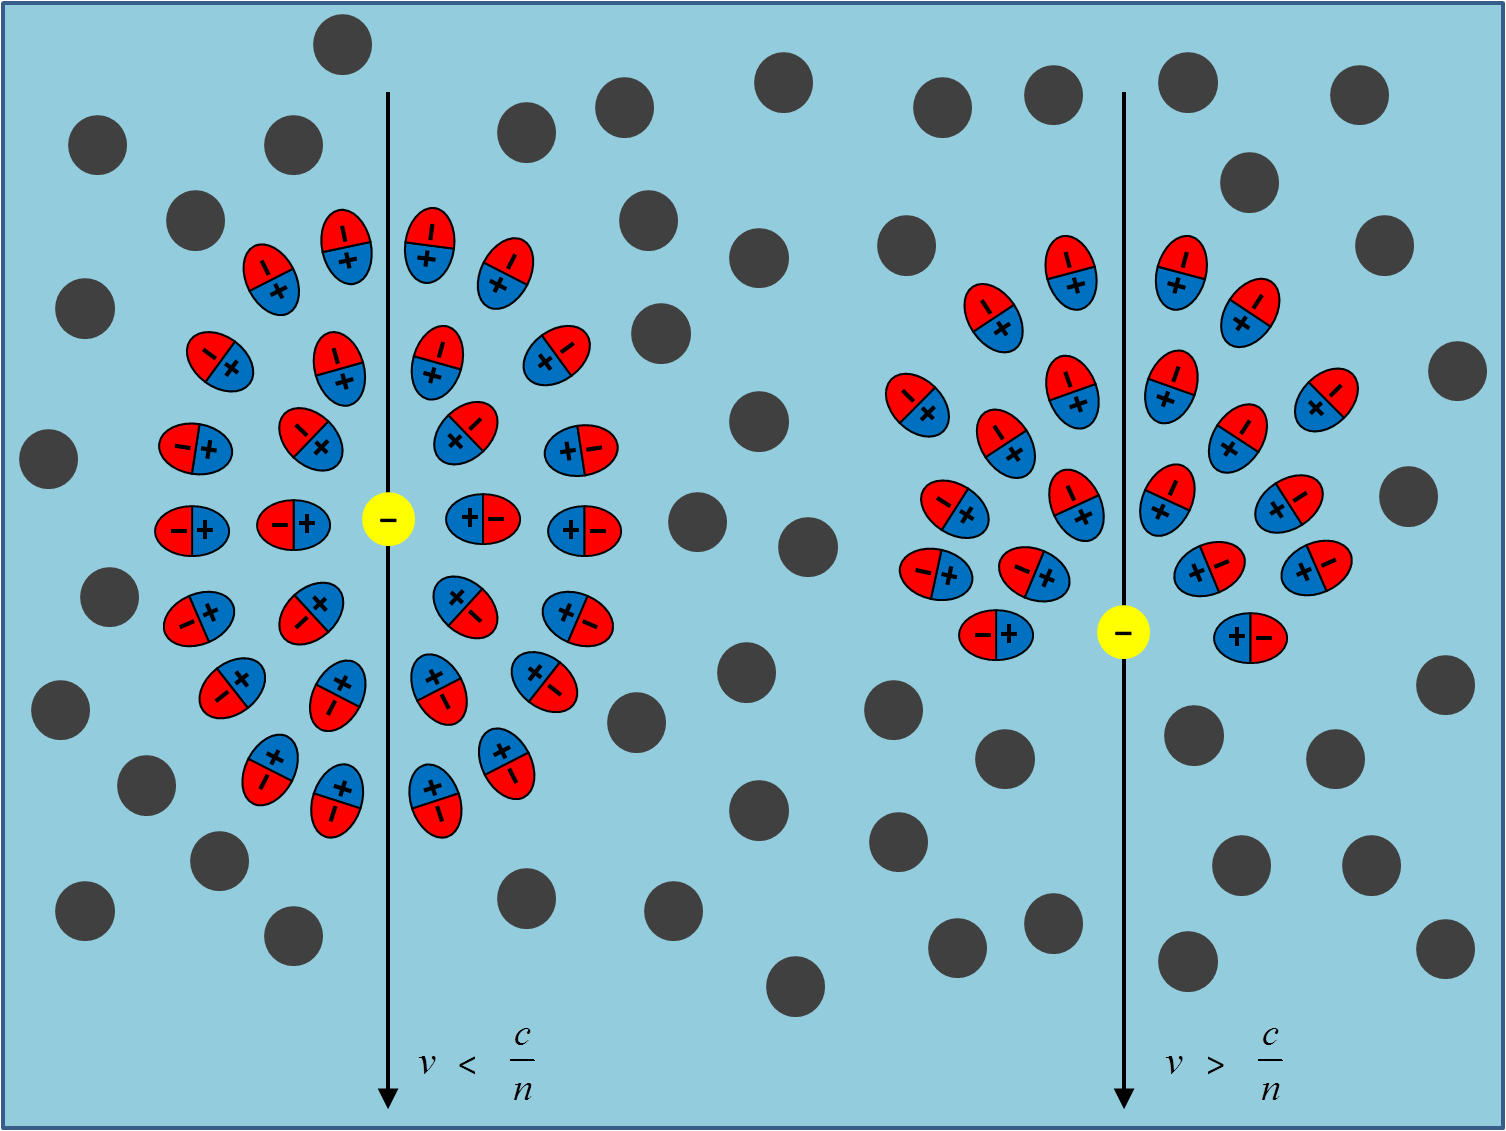
\includegraphics[width=\figwidth,height=\qfigheight]{\figures/hall-b/CCECPLOTS/cherenkov.pdf}
\caption[Illustration of Cherenkov Radiation]{\label{fig:clas.cc.dipole}Illustration of Cherenkov Radiation. Negative charged particle traveling through a medium with $v < c/n$ showing dipoles symmetrically arranged around particles path (left). Negative charged particle traveling through a medium with $v > c/n$ showing dipoles asymmetrically arranged around particles path given rise to dipole field(right). Image Source:~\cite{cherenkov_image}}
\end{center}\end{figure}

The generated dipole field radiates the energy contained in this disturbance producing a coherent shockwave, this is known as Cherenkov radiation. An analogy of this phenomena is the sonic boom created in air from an object traveling faster then the speed of sound. Just as the sound wave of a sonic boom travels slower than the traveling object, so does the light emitted from the dipole field. This reduction in velocity creates the wave front of a continuous light spectrum, see Fig~\ref{fig:clas.cc.angle}.
\begin{figure}[h!]\begin{center}
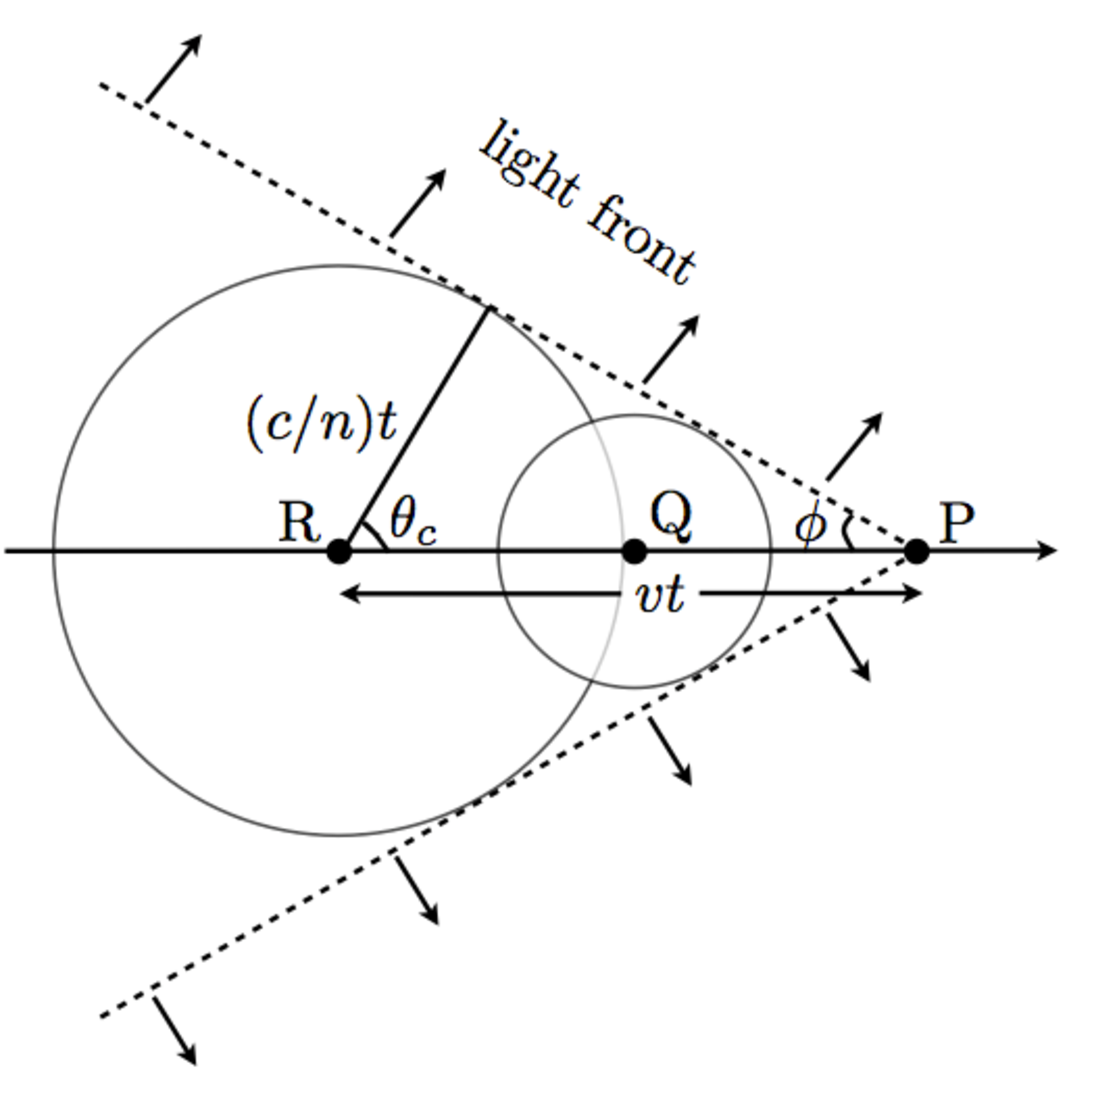
\includegraphics[width=\figwidth,height=0.75\hfigheight]{\figures/hall-b/CCECPLOTS/cc_wavefront_madeII.pdf}
\caption[Illustration of Cherenkov Angle]{\label{fig:clas.cc.angle}Illustration of Cherenkov Angle. When the particle has traveled the distance $\mathrm{RP =\nu t \rightarrow \beta c t}$, the photon (light front) has traveled $(c/n)t$.}
\end{center}\end{figure}

Inspecting Fig~\ref{fig:clas.cc.angle}, when the particle has traveled the distance $\mathrm{RP =\nu t = t \beta c}$, the photon has traveled $(c/n)t$, therefore
\begin{equation}\label{eq:cherenkov_eq}
 \mathrm{\cos\theta_{c} = \frac{(c/n)t}{t \beta c} = \frac{1}{n\beta}}
\end{equation}
and the threshold of Cherenkov radiation is 
\begin{equation}\label{eq:cherenkov_threshold}
 \mathrm{\beta_{th} > \frac{1}{n}}.
\end{equation}
Adding in quantum effects
\begin{equation}\label{eq:cherenkov_eq_quantum}
\mathrm{cos\theta_{c} = \frac{1}{n\beta} + \frac{\Lambda}{\lambda}\frac{n^{2} -1}{2n^{2}}}
\end{equation}
where
\begin{equation}\label{eq:cherenkov_eq_quantum_lambda}
\mathrm{\Lambda = \frac{\sqrt{1-\beta^{2}}}{\beta}\lambda_{0}} \ , 
\end{equation}
$\mathrm{\lambda =}$ wavelength of light in medium, and $\mathrm{\lambda_{0} }$ is the Compton wavelength 0.024 \AA. For practical cases, and using \abbr{CLAS}, the 2$^{nd}$ order term is negligible (n=1.00153). To illustrate that quantum effects are negligible, an electron traveling at threshold in \abbr{CLAS} \abbr{CC},
\begin{equation}
\mathrm{\beta_{th} > \frac{1}{n}} > 0.998472,
\end{equation}

\begin{equation}
\mathrm{\frac{\Lambda}{\lambda}\frac{n^{2} -1}{2n^{2}} =  1.07874 \cdot 10^{-9}}
\end{equation}
%

In \abbr{CLAS}, the Cherenkov counter (\abbr{CC}) is used to detect electrons and positrons while rejecting pions for momenta less than 2.5~GeV. The gas used in the \abbr{CC} for \g12 is perfluorobutane (C$_4$F$_{10}$) with an index of refraction of 1.00153. The threshold energy for producing Cherenkov radiation in C$_4$F$_{10}$ is
\begin{align}
\mathrm{E_{th} = \gamma_{th} m_{0}} \mathrm{ \ (Units \ of \ c)} \\
\mathrm{\gamma_{th} = \frac{n}{\sqrt{n^{2} -1}}} = 18.09
\end{align}
therefore the threshold energy of e$^{\pm}$ is 9.23~MeV while the threshold energy of $\pi^{\pm}$ is 2.52~GeV.
%
The number of photons emitted per unit length at threshold for electrons or positrons is;
\begin{align}\label{eq:cc.NPE}
\frac{dN}{dx} = 2\pi z^2 \alpha \frac{\sin \theta_{c}^2}{\lambda^2} d\lambda = 0.241246 \frac{d\lambda}{\lambda^2}
\end{align}
where $\alpha$ is the fine structure constant, $z =1$ for electrons and positrons, and $\lambda$ is the wavelength at which the photon is emitted. Table~\ref{tab:cc_npe} lists the number of photons/cm for various wavelengths of light for the midpoint of $\beta_{th}$ and a maximum velocity $\beta =1$. Table~\ref{tab:cc_npe} also lists the mirror reflectivity for that wavelength.
\begin{table}[h!]
\begin{minipage}{\textwidth}
\begin{center}
\begin{singlespacing}

\caption[Number of Photo-electrons per Unit Length in Cherenkov Detection]{\label{tab:cc_npe}Number of $\gamma$'s per unit length gas $C_4F_10$ \vspace{0.75mm}}

\begin{tabular}{c|c|c|c}

\hline
Wavelength~nm & \multicolumn{2}{c|}{$\frac{dN}{dx}$~photons/cm} & Mirror reflectivity~\cite{clas.cc}  \vspace{0.5mm} \\
\hline
&$\beta = \frac{1}{2}(1+\beta_{th})$& $\beta = 1$ \\
\hline
400-700 (visible) & $0.75$ & $1.5$ & 90\% \\
300-400 (near UV) & $0.6$ & $1.2$ & 85 - 90 \% \\
190-300 (near UV) & $1.4$ & $2.7$ & 20 - 85\% \\
\hline \hline
\end{tabular}
\end{singlespacing}
\end{center}
\end{minipage}
\end{table}
\vspace{20pt}


The \abbr{CC} subsystem is physically located in the space between Region 3 of the \abbr{DC} subsystem and the \abbr{TOF} in the forward region covering polar angles 8$^\circ$ to 45$^\circ$ in each sector when the target is at \abbr{CLAS} center. For \g12 since the target was placed 90~cm upstream, the polar coverage was approximately from 6$^\circ$ to 35$^\circ$ in the lab frame. The \abbr{CLAS} \abbr{CC}'s were fabricated as 6 independent identical sectors, with each sector divided into 18 regions of $\mathrm{\theta}$, and each $\mathrm{\theta}$ segment divided into 2 modules. Light from Cherenkov radiation is focused in $\mathrm{\phi}$ thus preserving information on the lepton polar angle $\theta$. The optical element of \abbr{CC} module comprises an assembly of one elliptical and one hyperbolic mirror providing primary light focusing into a  ``Winston" light collection cone, a  cylindrical mirror used to compensate for imperfections in the focusing, and a photomultiplier used to count the  number of photons in the light cone, see Fig~\ref{fig:clas.cc_array}. More information on the \abbr{CLAS} Cherenkov detector can be found in~\cite{clas.cc} 

The use of the \abbr{CC} was not included in the original proposals, however a significant drop in price on C$_4$F$_{10}$ just prior to the start of \g12 allowed the gas to be added at the last minute. The price drop was due to the recent availability of another, much cheaper gas that was demonstrated to have the same general properties as C$_4$F$_{10}$ and when \g12 contacted the original supplier of the C$_4$F$_{10}$ for a price match, they committed. 

\begin{figure}[h!]\begin{center}
\subfloat[]{
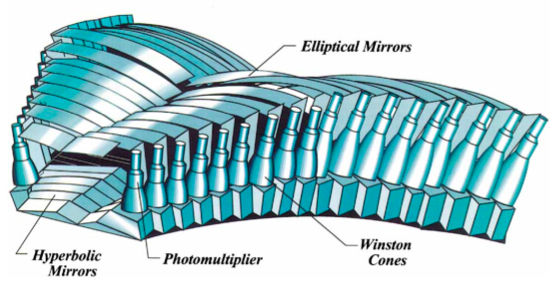
\includegraphics[width=\figwidth,height=0.5\hfigheight]{\figures/hall-b/CCECPLOTS/CCarray}\label{fig:clas.cc_array}
}\\
%[Schematic of one \abbr{CC} showing the 18 symmetrical, mirrored segments of the CLAS \abbr{CC}]
\subfloat[]{
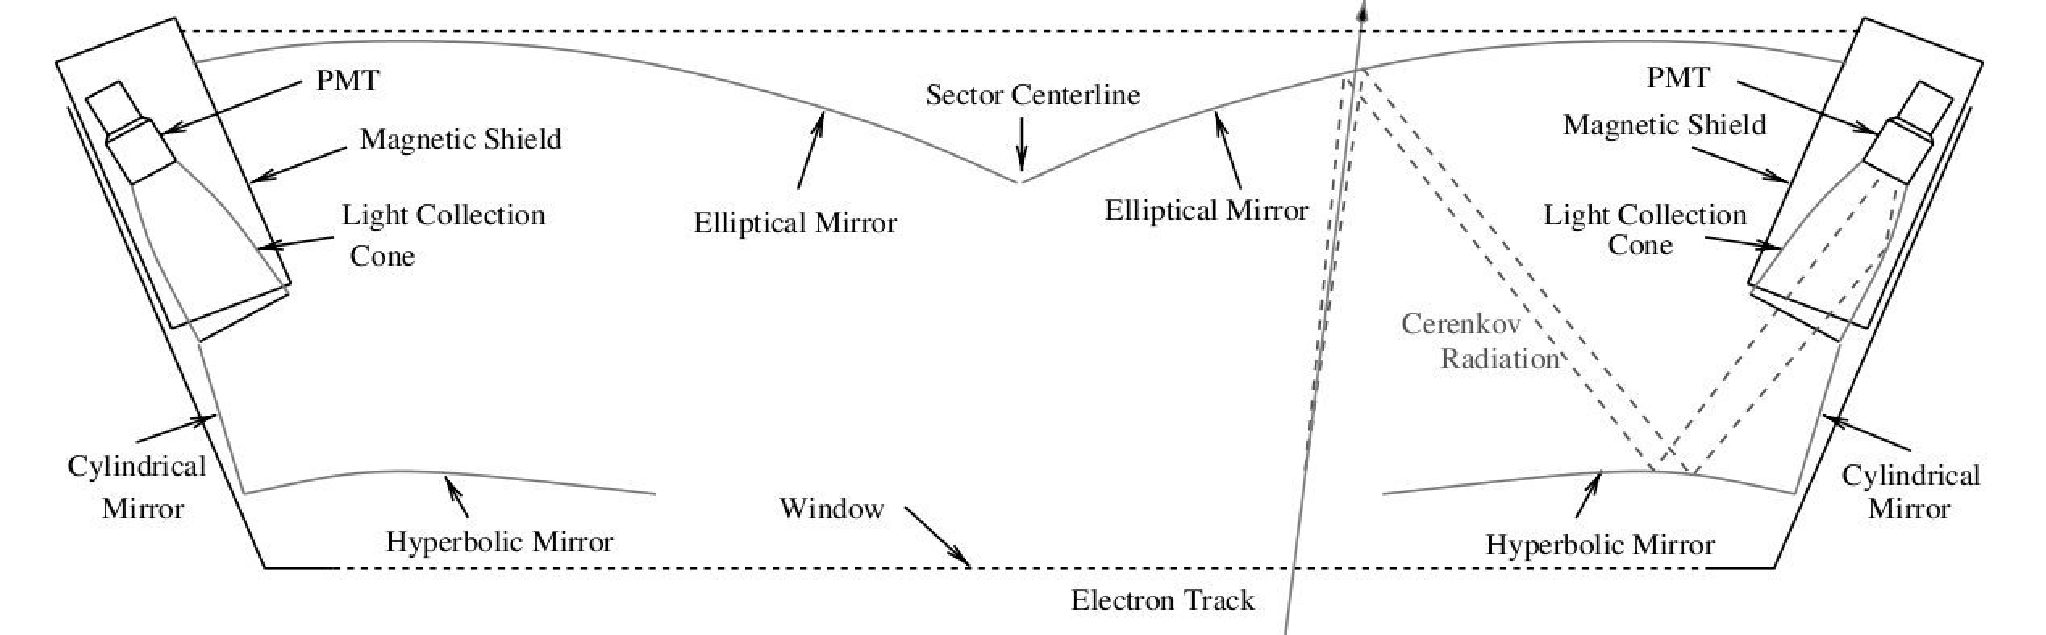
\includegraphics[width=0.9\columnwidth]{\figures/hall-b/cc_diagram.pdf}\label{fig:clas.cc}
}
\caption[Schematic of one \abbr{CC} showing the 18 symmetrical, mirrored segments of the CLAS \abbr{CC}]{Schematic of one \abbr{CC} showing the 18 symmetrical, mirrored segments of the CLAS \abbr{CC}~(a). Diagram of one segment of the Cherenkov counters with an electron entering from the bottom~(b).}

\end{center}\end{figure}






\FloatBarrier
\section{Time-of-Flight Detectors}\label{sec:clas.tof}

The \abbr{CLAS} time-of-flight \abbr{TOF} subsystem provides precise timing measurements of charged particles that transverse the \abbr{CLAS} detector to help determine the particle masses. The \abbr{TOF} subsystem was also used in the \g12 level 1 trigger (see Sec.~\ref{sec:data.trig}) to identify track candidates. The \abbr{TOF} is constructed of organic plastic scintillant (Bicron BC-408). Scintillation is a process undergone by material when radiation traverses a medium.
%
% At room temperature, all valence electrons of the scintillating material are in the $\mathrm{S_{0}}$ ground state. As a particle propagates through the material the incident radiation populates $\mathrm{S_{1}}$ states. Vibrational levels within $\mathrm{S_{1}}$ band decay radiation-less to $\mathrm{S_{1}}$  base states, which in turn decays under emission of light to the $\mathrm{S_{0}}$ band. The radiation-less decay from the excited $\mathrm{S_{1}}$ band to the ground $\mathrm{S_{1}}$ band is known as internal degradation and is responsible for the transparency of the scintillators to their own radiation. $\mathrm{S_{1}}$ can also decay to adjacent triplet levels however, this decay is highly forbidden by multipole selection rules. If this decay does occur, the decay energy is lower causing the decay time to be longer, see Fig.~\ref{fig:clas.scint_bands} for the illustration of this process. Depending on the properties of the scintillator, decay of fluorescent state in organic plastic scintillators have a typical time between 1-3~ns
%
%%\begin{figure}[h!]\begin{center}
%%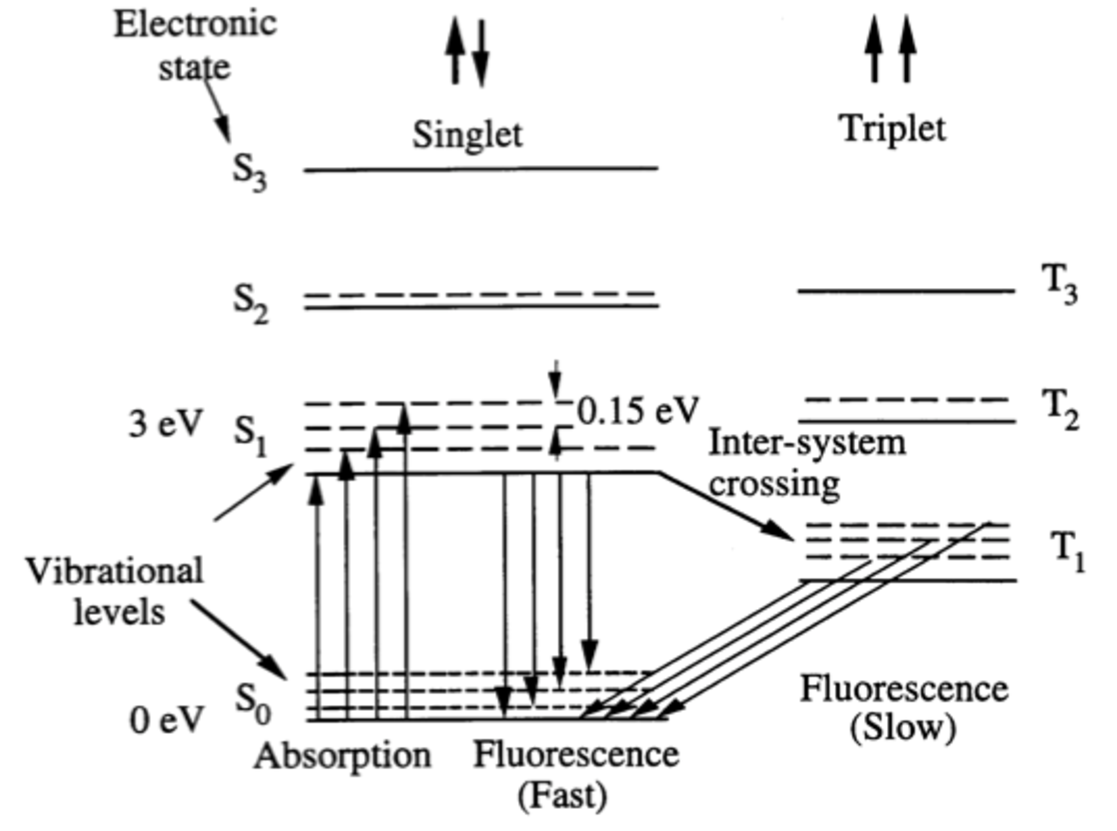
\includegraphics[width=\figwidth,height=0.5\hfigheight]{\figures/hall-b/CCECPLOTS/Calorimetry/scint.pdf}\label{fig:clas.scint_bands}\caption[Typical Energy Levels of scintillating material ]{Diagram of scintillating population of states. Image Source~\cite{vibe_levels}}
%%\end{center}\end{figure}
%\begin{figure}[h!]\begin{center}
%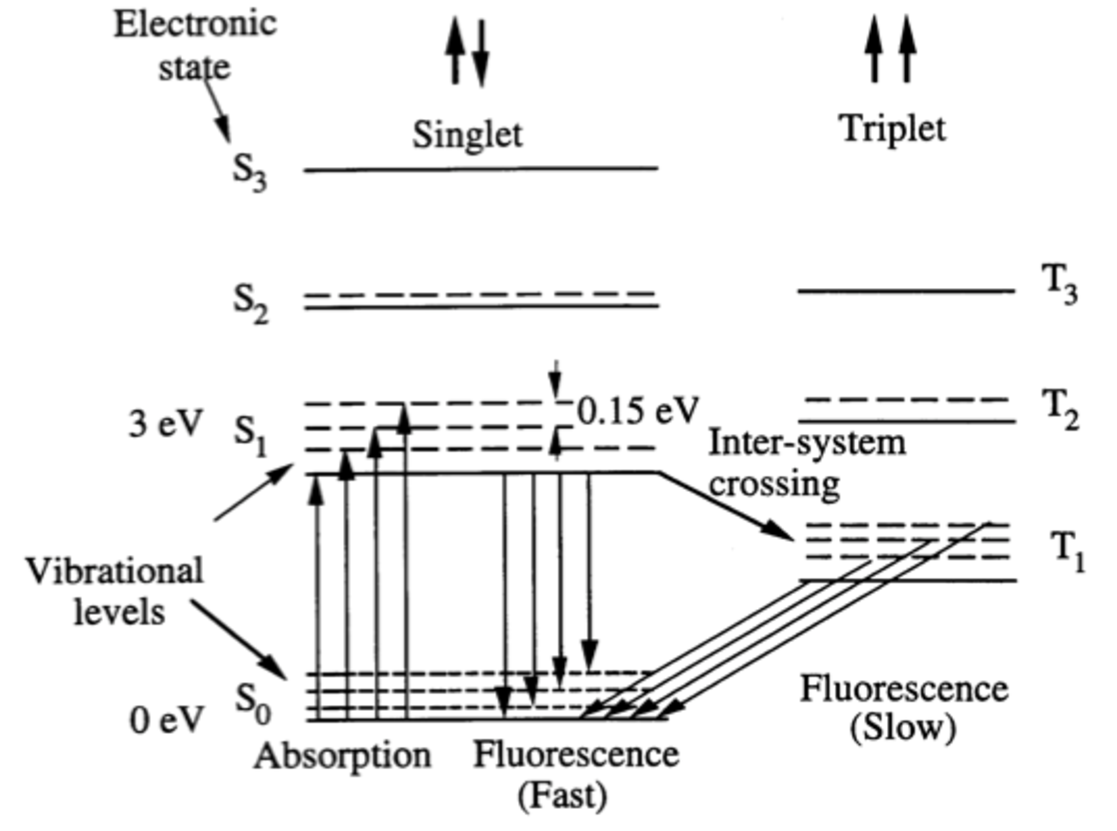
\includegraphics[width=\figwidth,height=0.5\hfigheight]{\figures/hall-b/CCECPLOTS/Calorimetry/scint.pdf}
%\caption[Typical Energy Levels of scintillating material ]{\label{fig:clas.scint_bands}Diagram of scintillating population of states. Image Source~\cite{vibe_levels}}
%\end{center}\end{figure}

The \abbr{TOF} subsystem is located between the \abbr{CC} and \abbr{EC} subsystems approximately 4~m from \abbr{CLAS} center, 5~m from the \g12 target. Each sector 57 scintillator paddles divided into two subgroups. The first subgroup subtends angles of 8.6$^\circ$ to 45.9$^\circ$ and consists of 23 scintillating paddles that are 15~cm in width. Each paddle is instrumented with two 2-in diameter \abbr{PMT}'s, see Fig~\ref{fig:clas.tof.paddles}. The first group was optimized for timing resolution while being cost-effective and covering a large area. The second group consists of 34 paddles that are 22~cm wide, covering polar angles from 45.9$^\circ$ to 142$^\circ$. Each paddle in this range is instrumented with two 3-in diameter \abbr{PMT}'s. All paddle bars are 5.08~cm thick for 100\% detection of minimum-ionizing tracks and a timing resolution of 150--200~ps.
%These forward angle counters \abbr{PMT}'s have a 15.9~cm$^2$ photocathode area which covers the 76.2~cm$^2$ cross-sectional area of the scintillator.
%These large angle counter \abbr{PMT}'s have a 30.2~cm$^2$ photocathode area which covers the 118.8~cm$^{\mathrm{2}}$ cross-sectional area of the scintillator.
\abbr{TOF} information is used to reconstruct a particle's mass is by measuring the difference between the event RF corrected start time and the time measured by the \abbr{TOF}, $t_{stsc}$. The RF corrected start time is the radio-frequency time (RF) from the accelerator beam aligned withe the event start time. Using this time, $t_{stsc}$, the length of trajectory to the \abbr{TOF}, $l_{stsc}$, and the speed of light $c$, the particles' velocity can be calculated as
\begin{equation}\label{eq:beta.cal}
\beta = l_{sc}/(t_{c}\cdot c)
\end{equation}
The particle's mass can be reconstructed from the measured velocity and momentum:
%Once the particles velocity is determined as well as the momentum, from the \abbr{DC} subsystem,  the particle mass can be reconstructed as 
\begin{equation}\label{eq:mass.cal}
m = p\sqrt{(1-\beta^2)}/\beta
\end{equation}

\begin{figure}\begin{center}
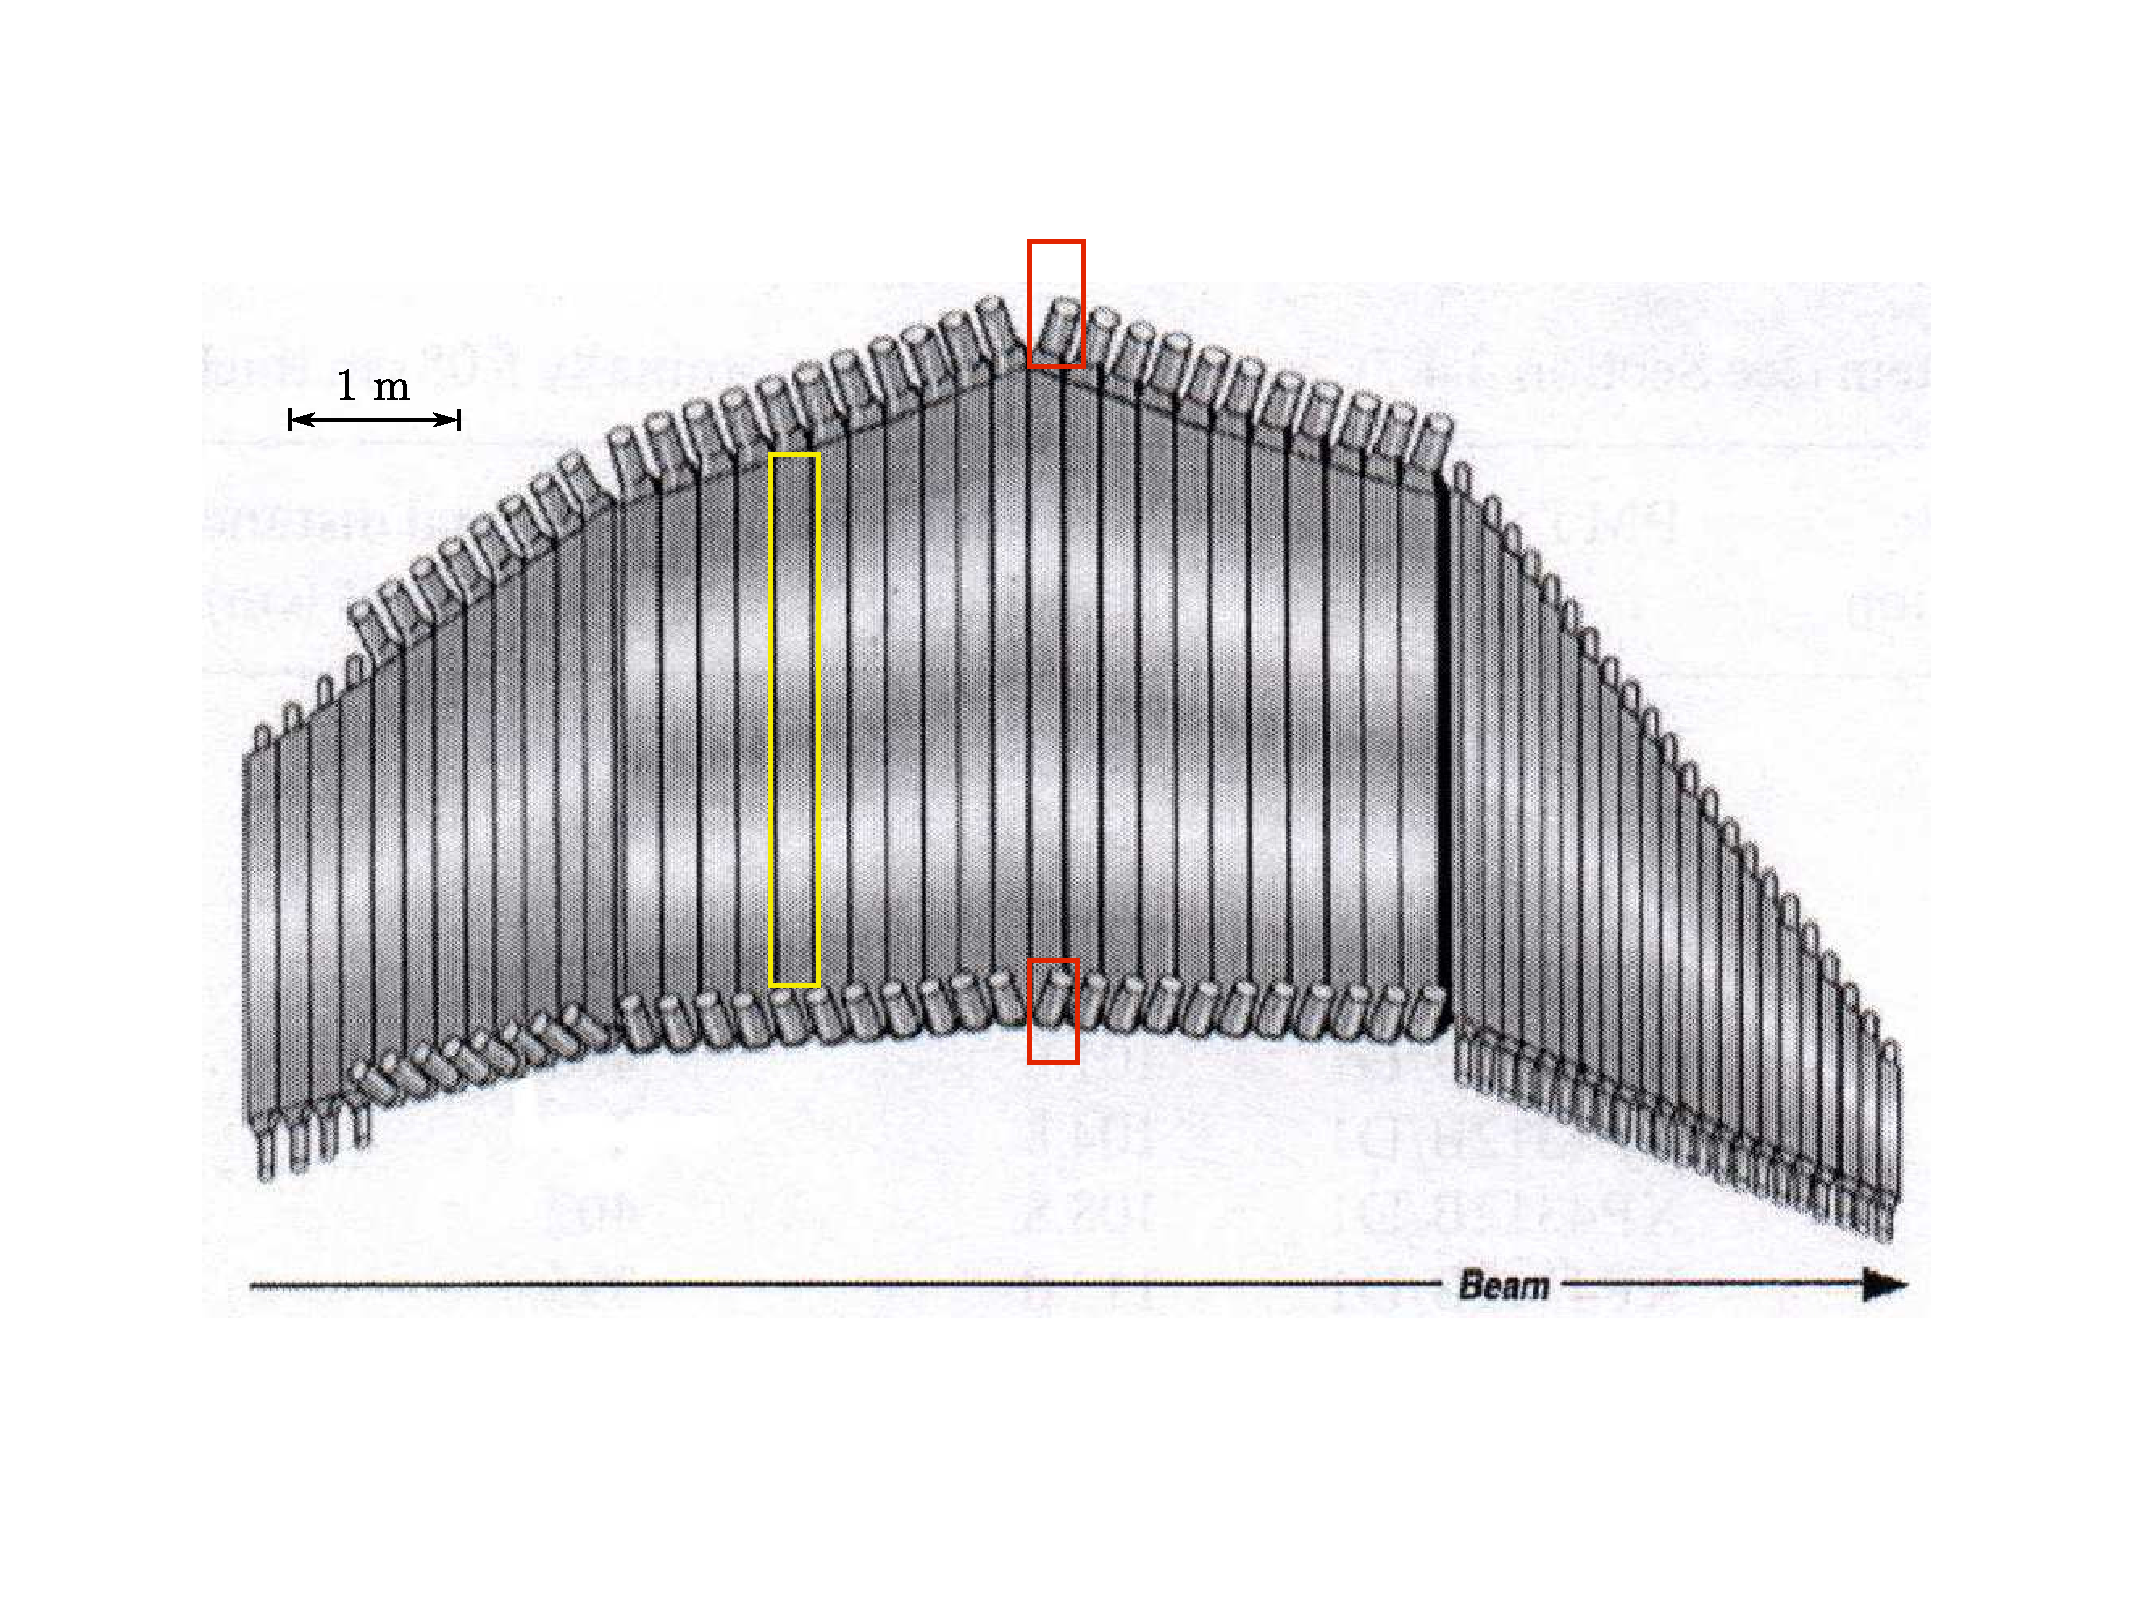
\includegraphics[width=\figwidth]{\figures/hall-b/tof_paddlesII.pdf}
\caption[Diagram of one sector of the time-of-flight (\abbr{TOF}) paddles]{\label{fig:clas.tof.paddles}Diagram of one sector of the time-of-flight (\abbr{TOF}) paddles. There are 57 scintillator paddles covering the entire acceptance region of the drift-chambers for each sector. \abbr{PMT}'s are outlined in red while a scintillator paddle is outlined in yellow.  Image Source:~\cite{clas.tof}}
\end{center}\end{figure}

\FloatBarrier
%\begin{figure}\begin{center}
%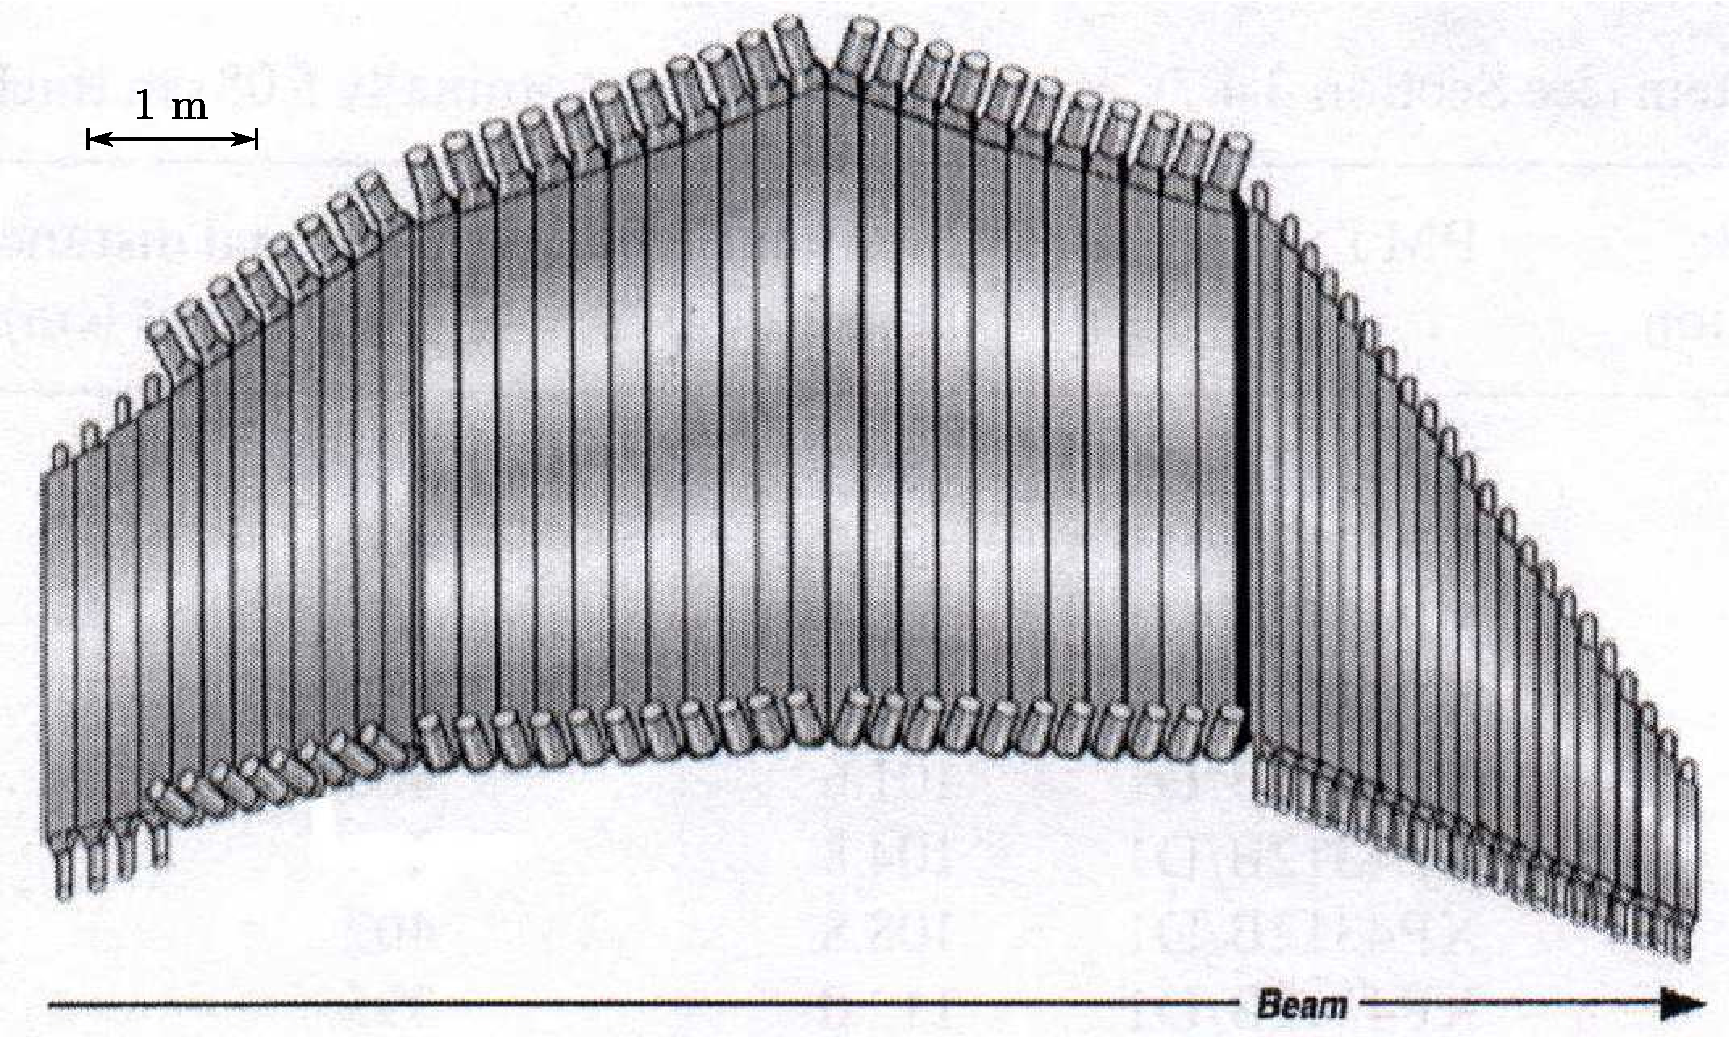
\includegraphics[width=\figwidth]{\figures/hall-b/tof_paddles.pdf}
%\caption[Time-of-Flight Paddles]{\label{fig:clas.tof.paddles}Diagram of one sector of the time-of-flight (\abbr{TOF}) paddles. There are 57 scintillator paddles covering the entire acceptance region of the drift-chambers for each sector.}
%\end{center}\end{figure}
%
%\begin{figure}\begin{center}
%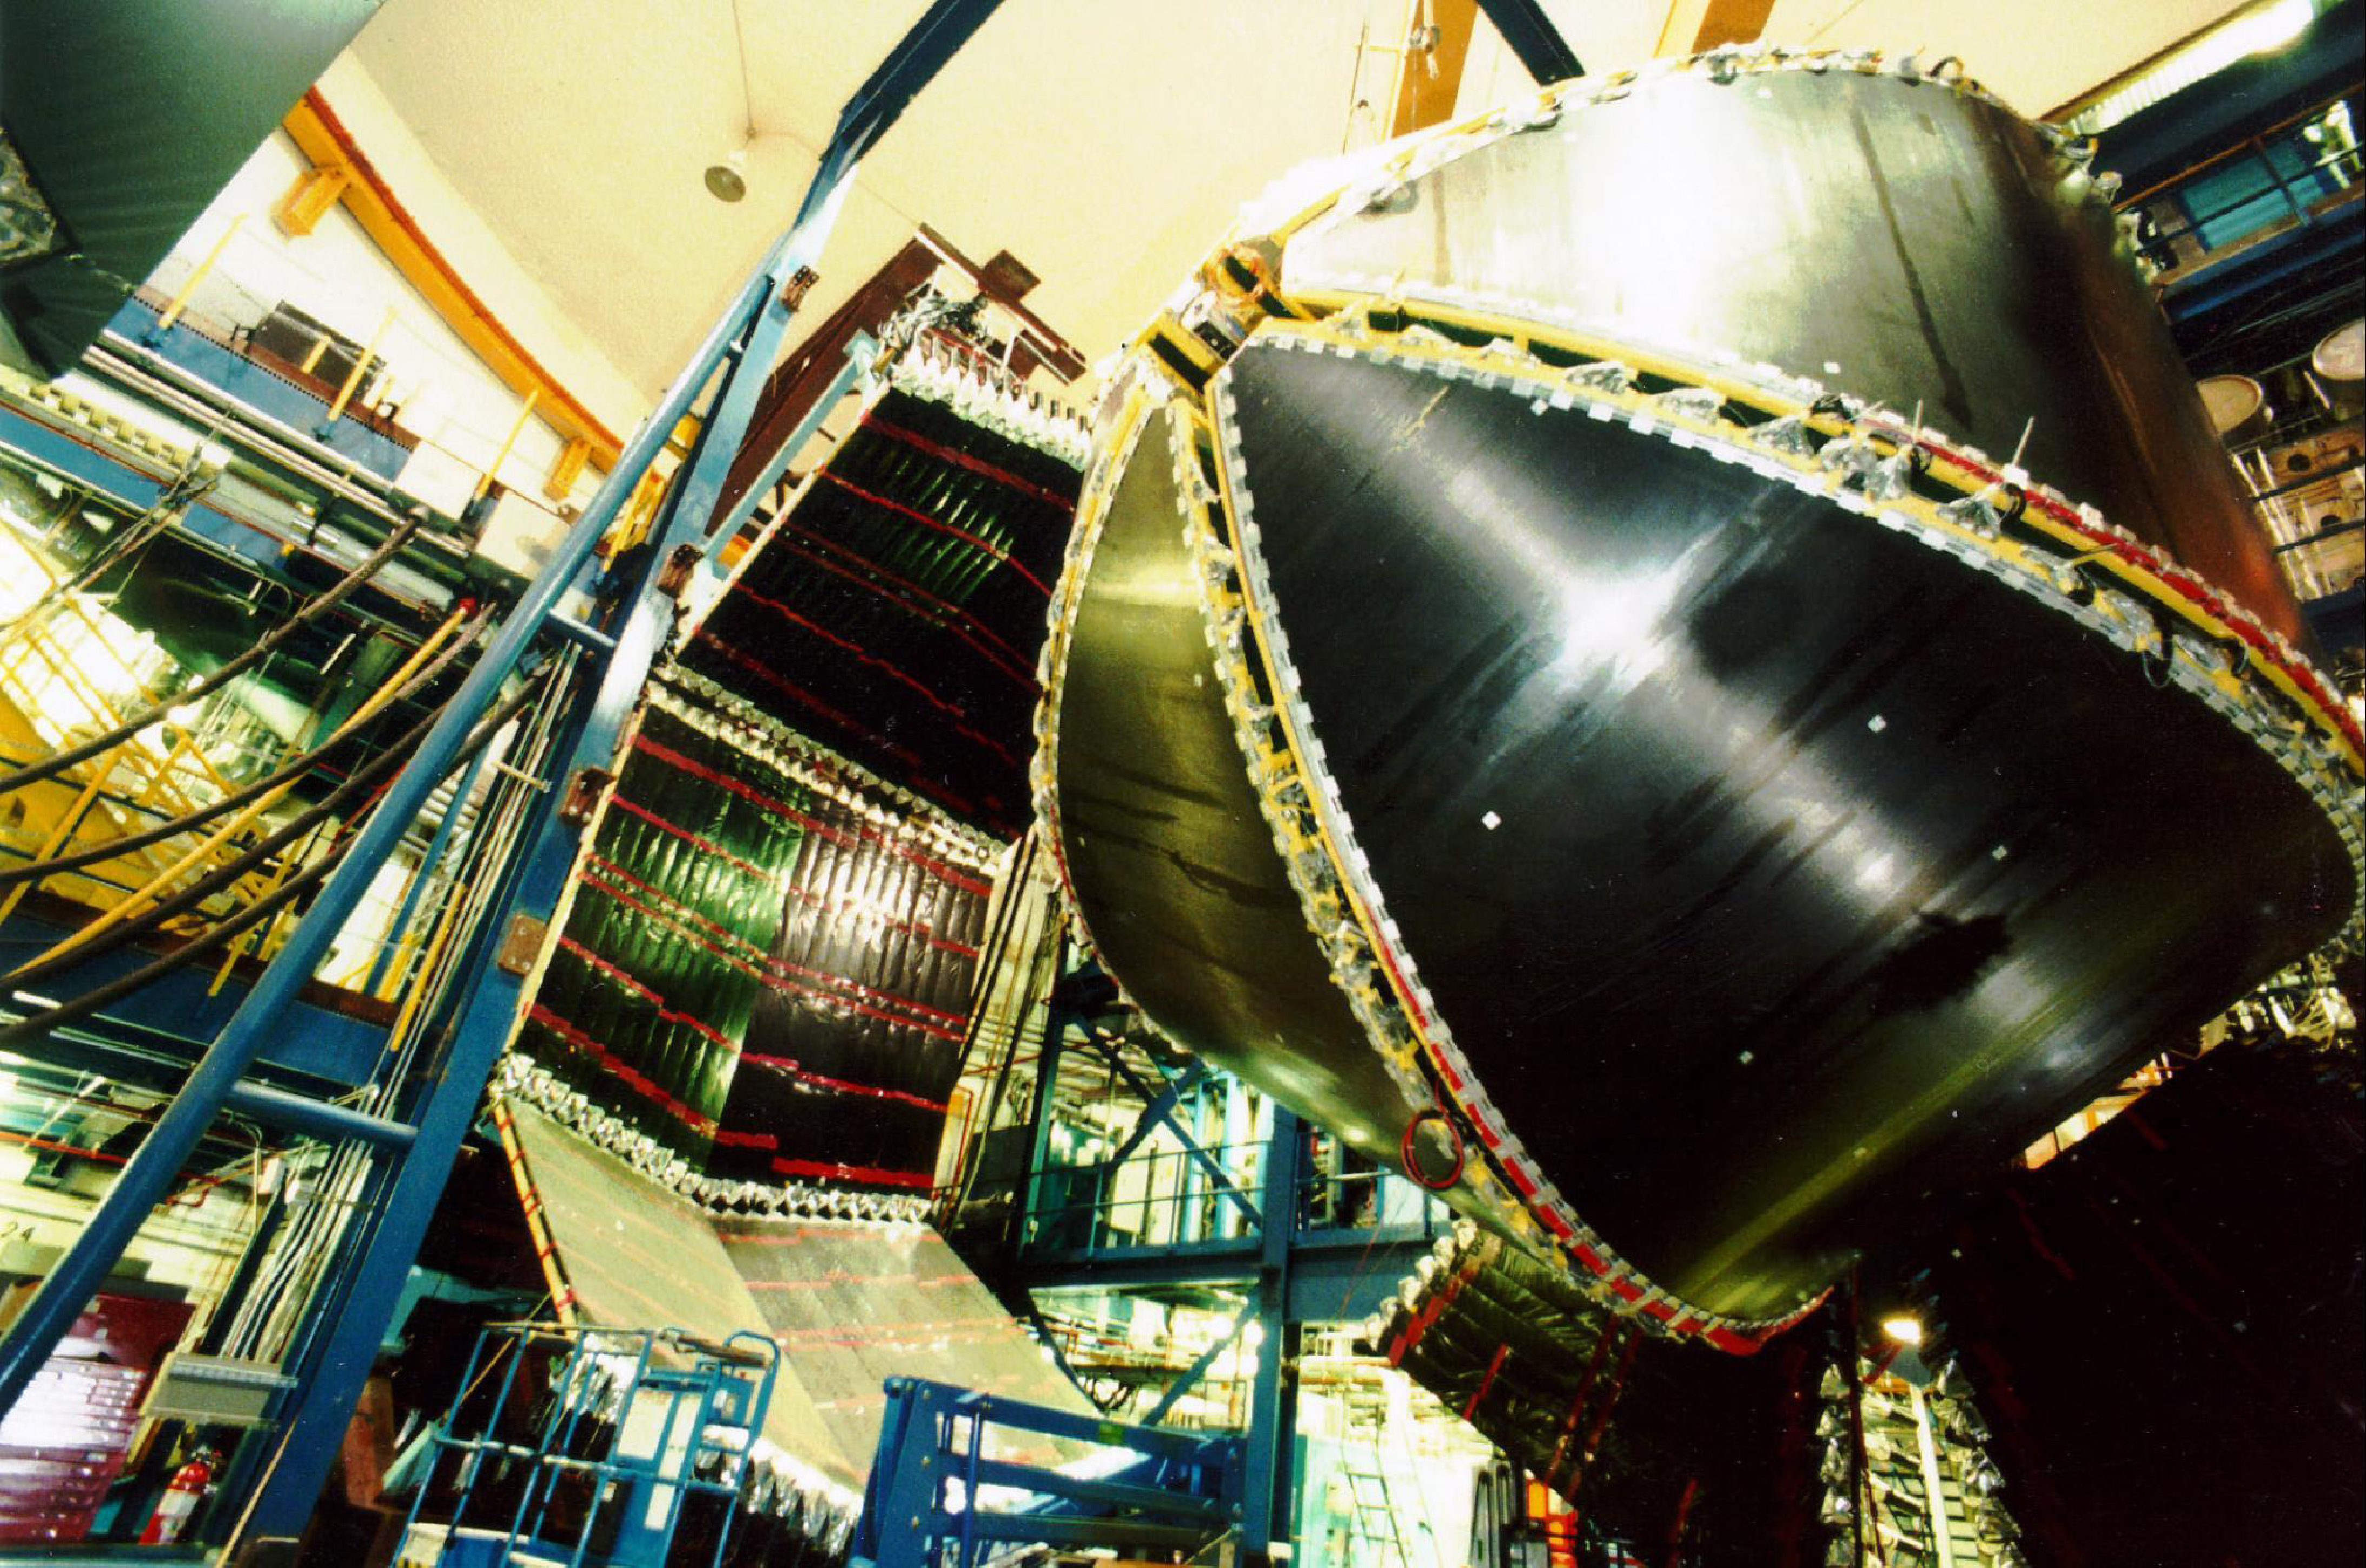
\includegraphics[width=0.8\columnwidth]{\figures/hall-b/clas_detector.pdf}
%\caption[\abbr{CLAS} Detector (photograph)]{\label{fig:clas.photo}The \abbr{CLAS} detector during a maintenance period where the time-of-flight ``shell'' (left) was pulled back from the drift-chambers (\abbr{DC}, right). The beam line enters from the lower right on the other side of the \abbr{DC}. The \abbr{TOF} paddles seen are the two center \emph{panels} shown in Fig.~\ref{fig:clas.tof.paddles} for three of the \abbr{CLAS} sectors.}
%\end{center}\end{figure}
%
%\begin{figure}\begin{center}
%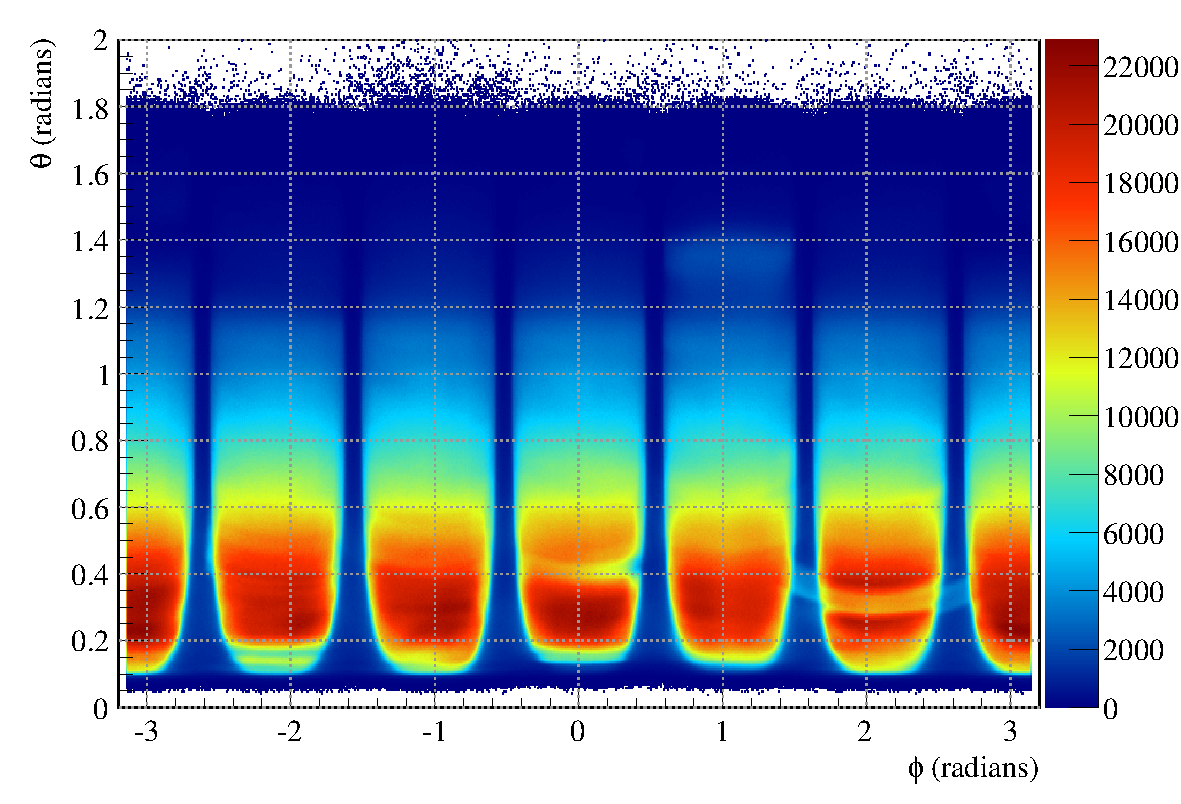
\includegraphics[width=\figwidth]{\figures/reconstruction/coverage_tof.pdf}
%\caption[Time-of-Flight Angular Coverage]{\label{fig:clas.tof.coverage}{\coloronline}Angular coverage in the lab frame of the tracks that had an associated time-of-flight hit. This can be interpreted as the total drift-chamber coverage of the \abbr{CLAS} detector.}
%\end{center}\end{figure}

\section{Electromagnetic Calorimeters}\label{sec:clas.ec}

The calorimetric method implies total absorption of the particle energy in a bulk of material followed by the measurement of the deposited energy. The process usually involves several layers of absorbers and detectors. Depending on the energies and species of particles there are different types of calorimeters. For instance, a 10~GeV muon will require 9~m of Fe or 8~m of Pb to absorb all the energy of the muon. However, a 10~GeV electron will only require 0.2~m of Pb to absorb all the energy.The Electromagnetic Calorimeter was built and used for detection of neutral particles as well as discrimination between electrons and pions.

%\begin{figure}[h!]\begin{center}
%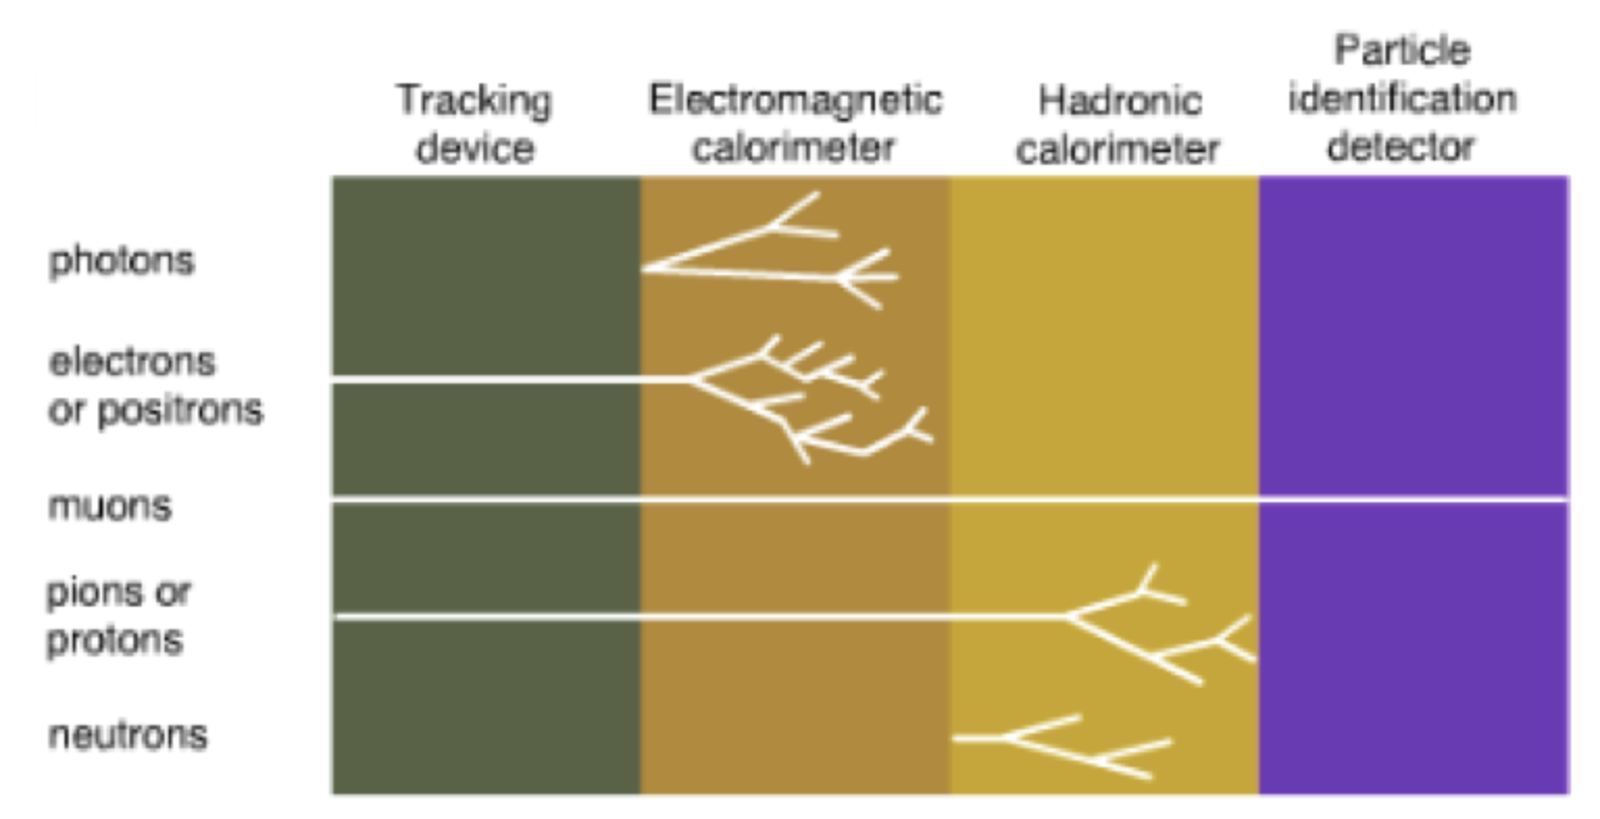
\includegraphics[width=\figwidth,height=\qfigheight]{\figures/hall-b/CCECPLOTS/Calorimetry/detectors.pdf}
%\caption[Types of Calorimeters]{\label{fig:clas.ec.calorim}Type of calorimeter depends on type of hadron detection Image Source:~\cite{C5}}
%\end{center}\end{figure}

\subsection{Electromagnetic Calorimeter}

At energies greater than 100~MeV, electrons lose their energy predominantly by bremsstrahlung while photons lose their energy by electron-positron pair production. The process of bremsstrahlung is electromagnetic radiation produced by the deceleration of an electron when deflected by an atomic nucleus i.e. $\mathrm{e Z \rightarrow Ze\gamma}$. Its cross-section is proportional to $\mathrm{Z^{2}}$ of the material the electron propagates through. The radiation loss of electrons with initial energy $E_0$ can be described as
\begin{align}\label{eq:electron_eloss}
-(\frac{dE}{dx})_{rad} = \frac{E}{X_{0}} \\ \vspace*{10 mm} E(x)=E_{0}e^{\frac{-x}{X_{0}}} 
\end{align}
where $X_{0}$ is the radiation length of the material the electron travels through. The process of pair production, $\gamma Z \rightarrow Ze^{+}e^{-}$ was discussed in Sec.~\ref{sec:intro.conversion}.
%, occurs when a photon with $E_0 > 2 m_e c^2$ converts into an electron and a positron. The cross section for this process can be simplified as
%\begin{equation}\label{pair_crosssection}
%\sigma_{\gamma\rightarrow e^+e^-} =  \frac{A}{N_{A} \rho \lambda_\gamma}  \ ,\ \lambda_\gamma = \frac{9}{7}X_0
%\end{equation}
%where $\lambda$ is also know as the interaction length, or mean free path, $\rho$ is the density of the material, $N_A$ is Avogadro's number and $A$ being the atomic mass of the material. The probability of pair production to occur is solely based on $X_{0}$, the radiation length of the medium and this probability can be expressed as
%\begin{equation}
%\frac{dP}{dx} = \frac{1}{\lambda_\gamma}\exp(\frac{-x}{\lambda_\gamma}) \ .
%\end{equation}

To explain how an Electromagnetic Calorimeter works, assume the absorber for the calorimeter is lead(Pb), Fig \ref{fig:clas.photon_processes} , \ref{fig:clas.electron_processes} depicts the processes for photons and electrons in Pb.
\begin{figure}[h!]\begin{center}
\subfloat[][]{
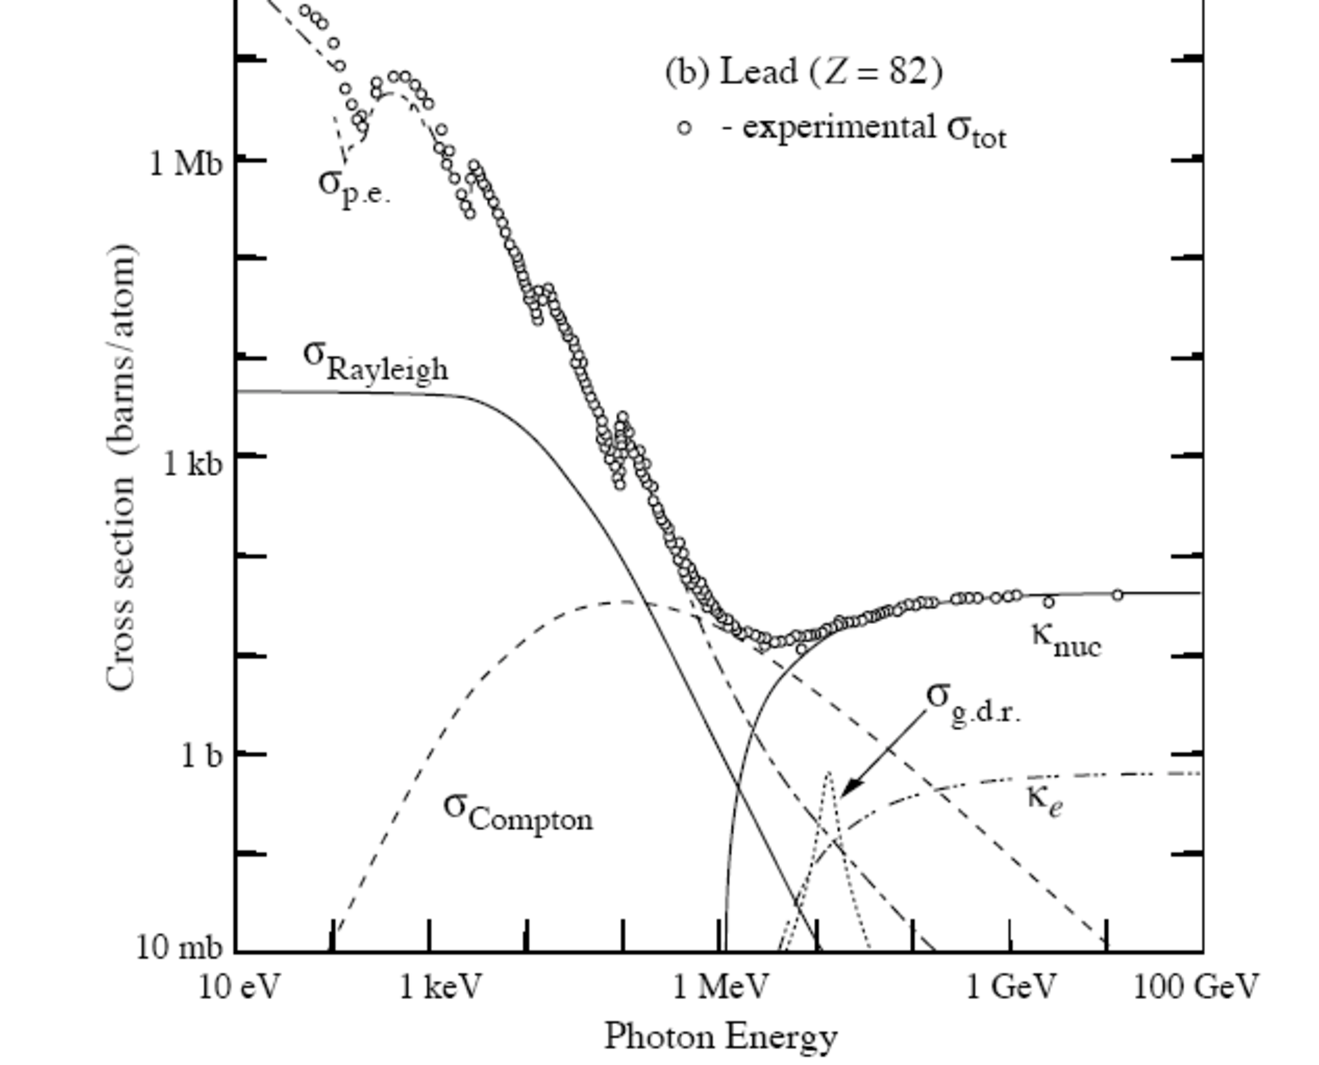
\includegraphics[width=0.45\columnwidth,height=0.5\hfigheight]{\figures/hall-b/CCECPLOTS/Calorimetry/PhotonRadiations.pdf}\label{fig:clas.photon_processes}
}
\subfloat[][]{
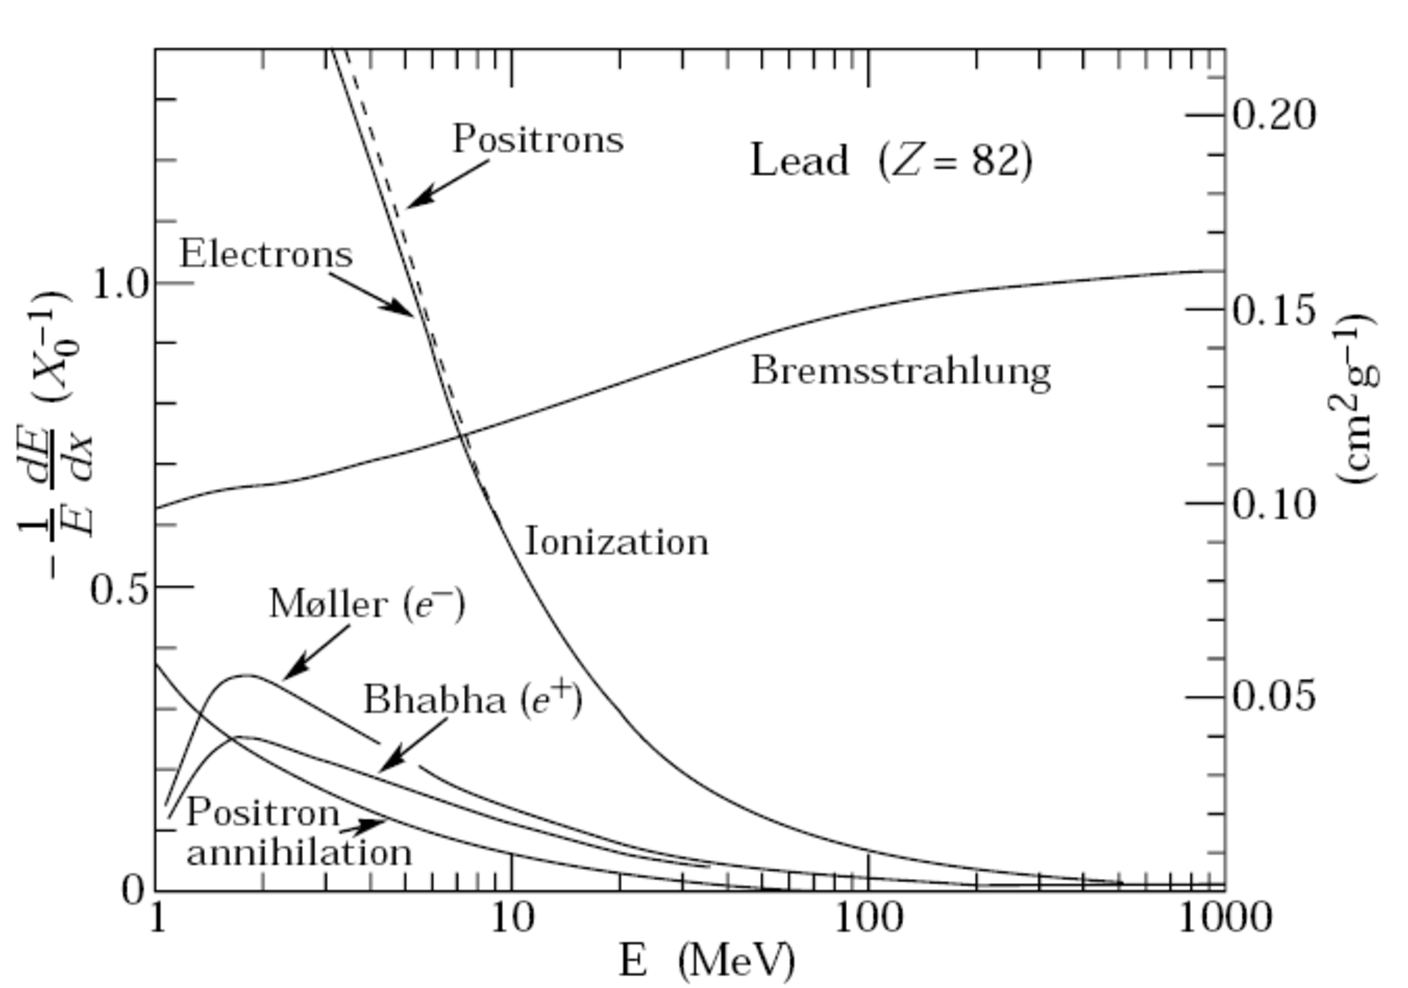
\includegraphics[width=0.45\columnwidth,height=0.5\hfigheight]{\figures/hall-b/CCECPLOTS/Calorimetry/EectronE2.pdf}\label{fig:clas.electron_processes}}
\caption[Photon and Electron processes in \abbr{Pb}]{Photon and Electron processes in \abbr{Pb}~(a) and (b) respectively. Images Source:~\cite{vibe_levels}} 

\end{center}\end{figure}
Lets start with a high energy electron $E_{0}$, after $1 X_{0}$, $\mathrm{1e^{-}}$ and $\mathrm{1 \gamma}$ are produced each with $\frac{E_{0}}{2}$, after $2 X_{0}$, $\mathrm{2e^{-}}$, $\mathrm{1e^{+}}$ and $\mathrm{1 \gamma}$ are produced each with $\frac{E_{0}}{4}$. Therefore after $tX_{0}$, there is a total of 
\begin{equation}
N(t)=2^{t}
\end{equation}
are produced each with
\begin{equation}
E(t) = E_{0}2^{-t}.
\end{equation}
The multiplication of the shower particles continue as long as
\begin{equation}
\frac{E_{0}}{N} > E_{c},
\end{equation}
where $E_{c}$ is the critical energy for showers to propagate,
\begin{align}
E_{c}  = E_{0}2^{-t_{max}} \\
N_{max}=\frac{E_{0}}{E_{c}}
\end{align}

\begin{figure}[h!]\begin{center}
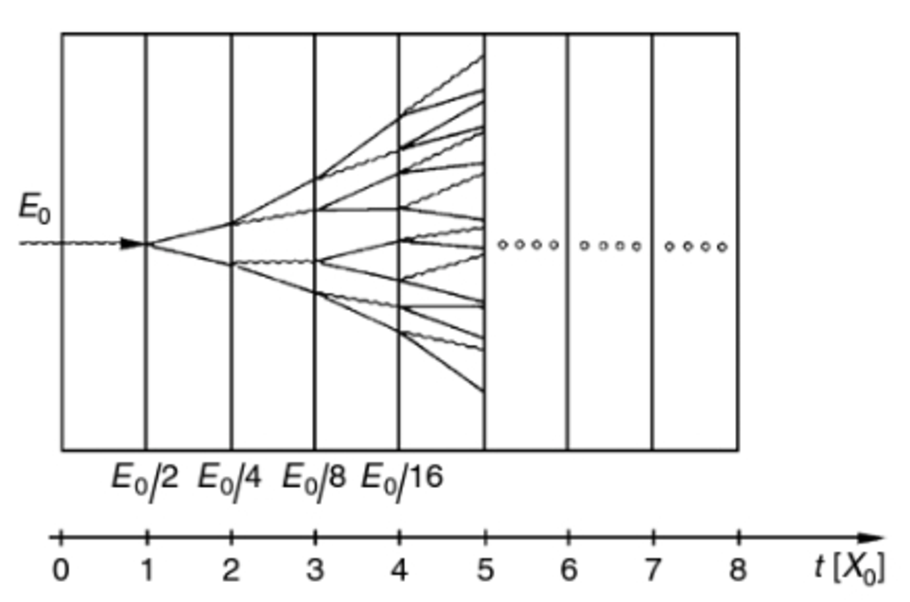
\includegraphics[width=\figwidth,height=\qfigheight]{\figures/hall-b/CCECPLOTS/Calorimetry/cascade.pdf}
\caption[A simple Electromagnetic shower in a calorimeter]{\label{fig:clas.ec.shower}{A simple Electromagnetic shower in a calorimeter} Image Source:~\cite{vibe_levels} }
\end{center}\end{figure}

When a particle falls below critical energy, absorption processes (ionization, Compton and photoelectric) start to dominate the processes for photons and electrons. This leads to
\begin{equation}
t_{max} = \frac{ln(\frac{E_{0}}{E_{c}})}{ln2}.
\end{equation}
At the shower maximum $\mathrm{e^{\pm}}$ will stop within $1X_{0}$ however, photons at critical energy will penetrate further. To absorb 95\% of photons produced in the shower maximum, an additional 7-9$X_{0}$ is necessary. The semi-empirical value for $\mathrm{e^{\pm}}$ $E_c$ in Pb is,
\begin{equation}
E_{c}  \thickapprox \frac{610 MeV}{\mathrm{Z} - 1.24} = 7 MeV 
\end{equation}
which results in $t_{max} \thickapprox 9.7 X_{0}$ for electrons at 6 GeV.

The process shown in Fig~\ref{fig:clas.ec.shower} is a very crude and simple model of an actual shower shown in Fig~\ref{fig:clas.ec.showerII}, but the simple model correctly describes the important features of Electromagnetic Calorimeters
\begin{itemize}
\item The total calorimeter thickness should be more than 10-15~$X_0$ in order to absorb almost all of the energy of an incident photon
\item The position of the shower maximum increases with energy, therefore the thickness of the calorimeter should increase as the logarithm of the energy.
\item If there is energy leakage, it is caused by photons escaping the calorimeter at the sides or at the back.
\end{itemize}

 
\begin{figure}[h!]\begin{center}
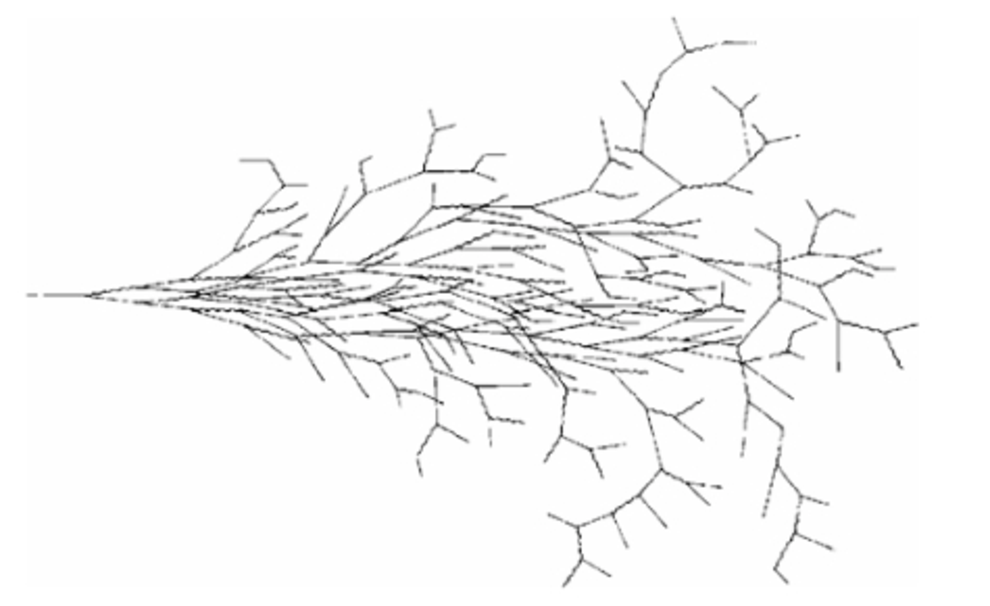
\includegraphics[width=\figwidth,height=\qfigheight]{\figures/hall-b/CCECPLOTS/Calorimetry/cascadeII.pdf}
\caption[A real Electromagnetic shower in a calorimeter]{\label{fig:clas.ec.showerII}{A real Electromagnetic shower in a calorimeter} Image Source:~\cite{vibe_levels} }
\end{center}\end{figure}

\subsection{The \abbr{CLAS} Electromagnetic Calorimeter}

The \abbr{CLAS} electromagnetic calorimeter (\abbr{EC})\cite{clas.ec}, shown in Fig.~\ref{fig:clas} was designed with the following criteria;
\begin{itemize}
\item $\mathrm{e/ \gamma}$ energy resolution $\sigma /E \leq 0.13/ \sqrt{E(GeV)}$
\item Position resolution $\delta r \approx 2cm \ at \ 1GeV$
\item $\mathrm{\pi / e}$ rejection greater than 99\% at $E \geq$1~GeV
\item Fast ($\textless$ 100 ns) total energy sum for the event trigger
\item Mass resolution for 2-photon decays $\delta m / m \leq 0.15$ 
\item Neutron detection efficiency $\textgreater$  50\% for  $E \textgreater$  0.5~GeV
\item Time-of-flight resolution $\approx$ 1 ns
\end{itemize}

The \abbr{EC} consists of alternating layers of Pb (absorber) and scintillator (detector). The lead to scintillator ratio of 0.2, i.e. 40 cm of scintillator, 8 cm of lead (16 $X_{0}$), was chosen so one third of the showering particle's energy is deposited into the scintillator. There are six triangular \abbr{EC} modules, one per sector, each a sandwich constructed of 39 layers. A layer is considered to be 10~mm thick BC412 scintillator followed by 2.2~mm lead. Each scintillator is made of 36 strips parallel to one side and are turned 120$^\circ$ from each other for each $u$, $v$ and $w$ view, 13 layers per view. The \abbr{CLAS} \abbr{EC} is subdivided into two stacks, inner and outer. The inner stack comprises of 8 layers while the outer stack comprises 5 logical layers. Each module contains 36(strips)x3(views)x2(stacks) therefore 216 \abbr{PMT}'s were needed per module, 1296 \abbr{PMT}'s total for \abbr{CLAS} \abbr{EC}, and 8424 scintillator strips. 

\begin{figure}[h!]\begin{center}
\subfloat[][]{
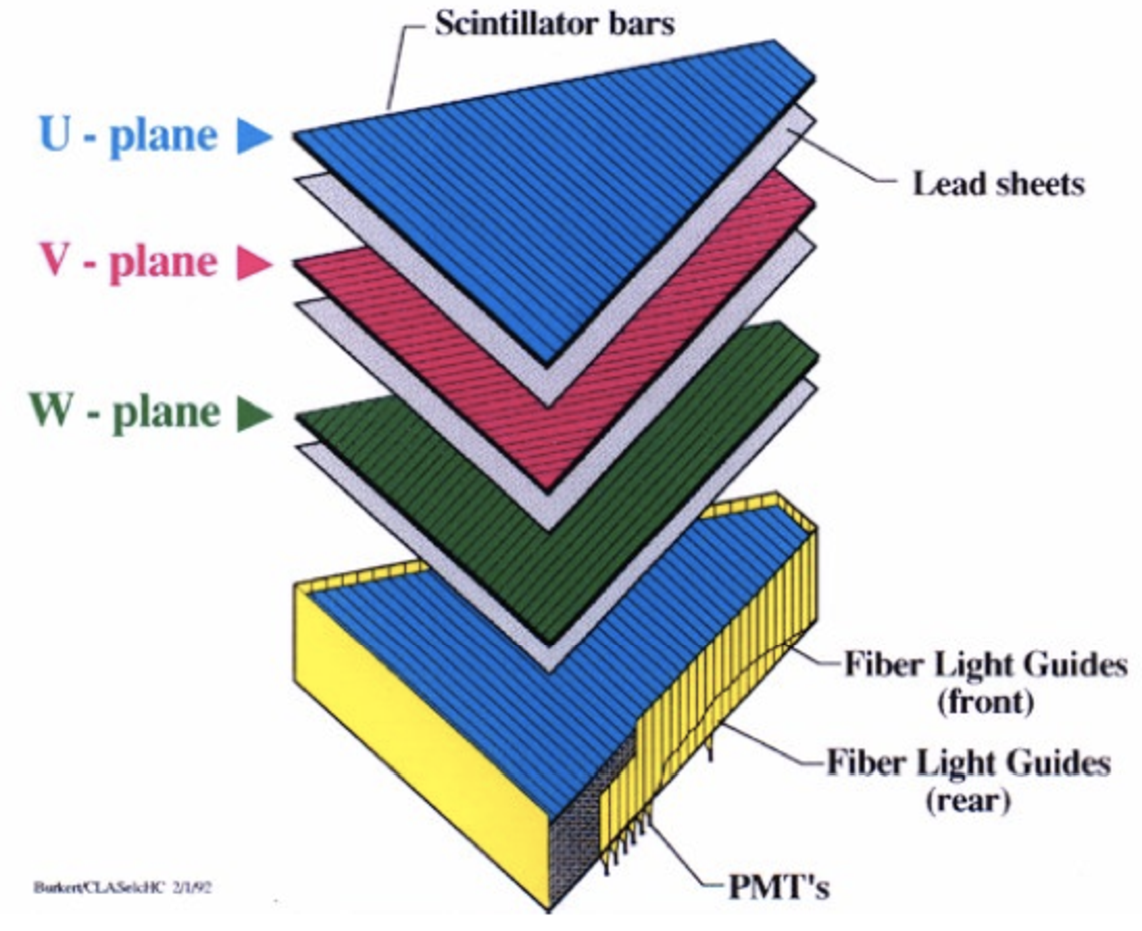
\includegraphics[width=0.8\columnwidth,height=0.75\hfigheight]{\figures/hall-b/CCECPLOTS/Calorimetry/CLASEC.pdf}\label{fig:clas.ec}
}

\subfloat[][]{
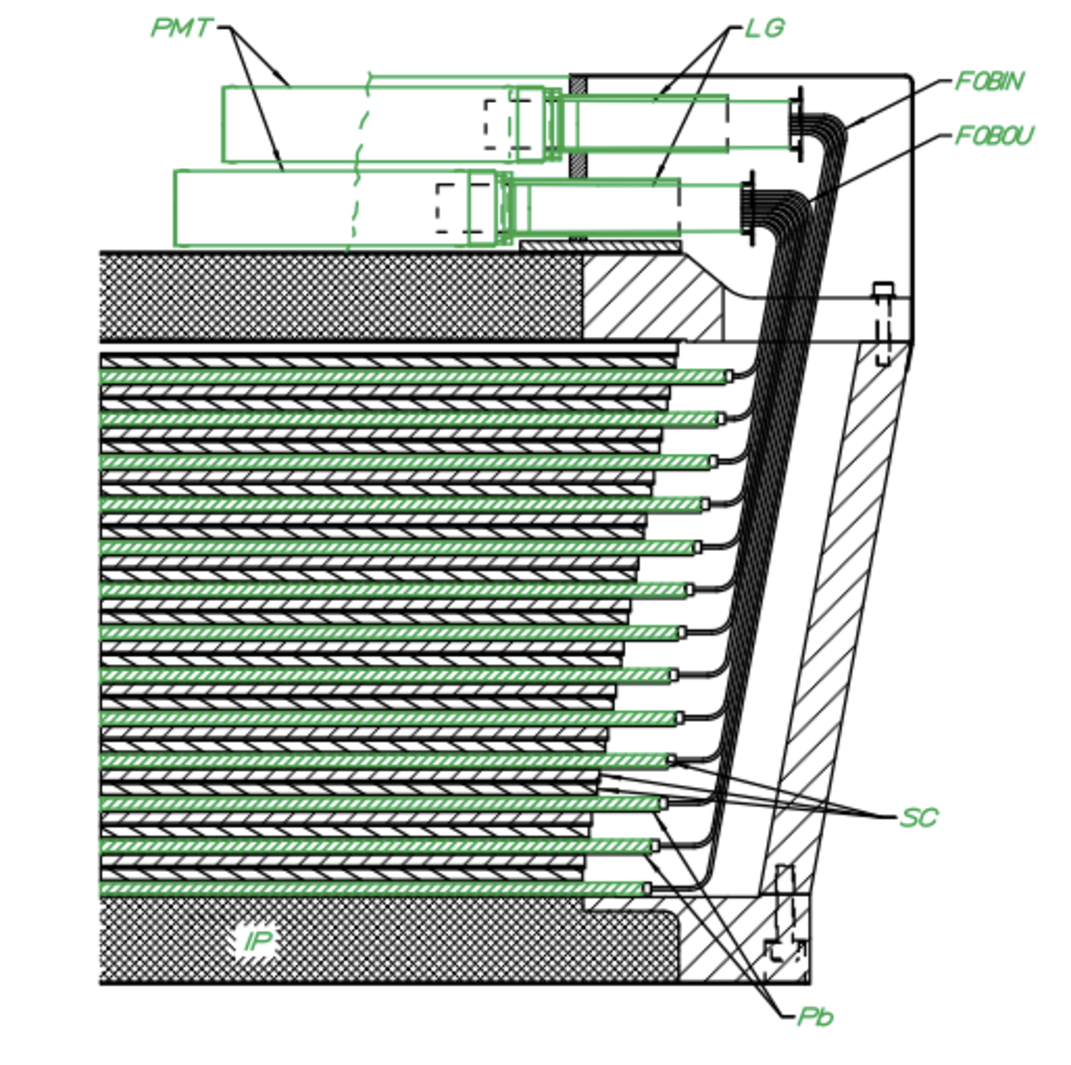
\includegraphics[width=0.8\columnwidth,height=0.75\hfigheight]{\figures/hall-b/CCECPLOTS/Calorimetry/CLASECSIDE.pdf}\label{fig:clas.ec.side}}
\caption[Separated view of one sector of the forward electromagnetic calorimeter (\abbr{EC}) showing the three planes ($u$, $v$, $w$) of scintillator-lead pairs which make up one of the 13 logical layers]{Separated view of one sector of the forward electromagnetic calorimeter (\abbr{EC}) showing the three planes ($u$, $v$, $w$) of scintillator-lead pairs which make up one of the 13 logical layers~(a). Side view of one plane of the forward electromagnetic calorimeter (\abbr{EC}) showing the the 13 logical layers, placement of the \abbr{PMT}'s and light guides~(b). Image Source: \subref{fig:clas.ec}~\cite{clas.ec} , \subref{fig:clas.ec.side}~\cite{clas.ec} respectively.} 

\end{center}\end{figure}

Using the three layers in each logical layer to provide pixel-like information, the transverse shower development for a given particle can be determined. All final-state photons were identified in the \abbr{EC} if no charged tracks have been associated with an energy deposit and also the velocity, $\beta$, of the particle exceeds 0.9c. Particles with $\beta <$~0.9c are neutron candidates.
%The difference in energy deposit between the inner and outer layers provides separation of electrons from pions in the reconstructed data for energies less than 2.8~GeV. For energies greater than 2.8~GeV, identification of pions and electrons are obtained by comparing the energy deposited in the \abbr{EC} with the momentum determined from the \abbr{DC}.


